\chapter{Topic modelling}\label{ch:topicmodelling}
Once extensively analysed the structure of the dataset, the goal becomes to develop a machine learning method to learn the hidden structure of the data.

%%intro
Remembering that in chapter~\ref{ch:structure} it emerged some kind of structure behind data, where each tissue seemed to be sampled by a different power law, a topic modelling approach is here proposed. Topic modelling has been developed and studied to approach linguistics problems, so this algorithm was developed considering words and books in input, links represent the abundance of a word in a book. In chapter~\ref{ch:structure} was evident that there are many similarities between data considered in this work and linguistics' corpora. Referring to data used in this project \textbf{samples} will be the documents and \textbf{genes} will be the words. It is expected that topics represent some properties of the system due to the gene expression distribution in samples.

The idea is that behind data there are hidden variables that describe the relationship between the genes and the samples. Let's call these variables topics.
Firstly it is necessary to build a bipartite network of genes and samples, then nodes are linked considering the gene expression value in the dataset.
\begin{figure}[htb!]
    \centering
    \includegraphics[width=0.7\linewidth]{pictures/topic/bipartite.pdf}
    \caption{An example of a bipartite network. Samples are on the left, genes are on the right. Each link is weighted by gene expression value. On the left side, all nodes of the same colour are clusters of samples. On the right side, all nodes with the same colour are a set of genes, also known as topics.\\
    Blue lines represent the cluster structure, each blue squared-dot is a set of nodes, lines delineate the hierarchical structure.\\
    It is clear in the middle the network separation between genes and samples.}
    \label{fig:topic/bipartite}
\end{figure}

The output of this kind of models consists of sets of genes, the topics, with a probability distribution $P(\text{gene} | \text{topic})$ and probability distributions of these topics inside each sample $P(\text{topic} | \text{sample})$, together they give the relationship between a \textit{sample} and a \textit{gene}.

In this work, an innovative and recent approach to topic model is proposed. The algorithm was presented by~\cite{gerlach2018network} and~\cite{Peixoto2017} explain it in details. This model is an evolution of a stochastic block model~\cite{Holland1983}. It is called hierarchical Stochastic Block Model (hSBM).

The ultimate goal is to be able to separate healthy and diseased samples then find and separate well-known tumour types and finally extend the actual knowledge and retrieve the tumour sub-types.

One of the advantages of this particular algorithm is that it is hierarchical, so it applies community detection at different layers of resolution. So the output has got different resolutions and different number of clusters at each layer . One extreme layer is the one which separates genes ($\simeq$ words) and samples ($\simeq$ samples), by definition; in other layers, it is possible to have few big clusters until the other extreme were the number of clusters is comparable with the number of nodes.
\begin{figure}[htb!]
  \centering
  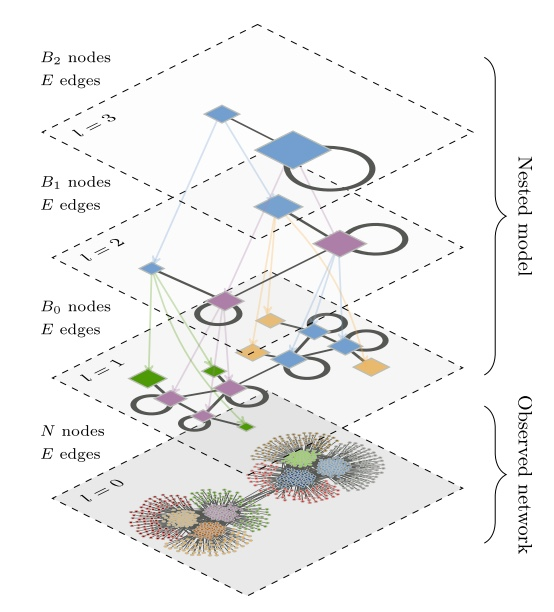
\includegraphics[width=0.6\linewidth]{pictures/topic/peixioto_hierarchic.jpg}
  \caption{Example of a hierarchical structure. At $l=0$ the number of cluster is comparable with the number of nodes, is the situation with many small clusters. Then they're merged in bigger clusters at other layers of the hierarchy.}
  \label{fig:topic_peixioto_hierarchic}
\end{figure}

What the algorithm does is to run a sort of Monte Carlo simulation and find the best partition of the data.
The probability that the hidden variables $\theta$ describe the data $G$ $P(\theta | G)$ can be written as a likelihood times a prior probability as
\[P(\theta|G)=\frac{P(G|\theta)\overbrace{P(\theta)}^{prior}}{\underbrace{P(G)}_{\sum_{\theta}P(G|\theta)P(\theta)}}.\]
It is possible to define a description length
\[
\Sigma=-lnP(G|\theta)-lnP(\theta),
\]
so that $P(\theta | G)\propto e^{-\Sigma}$.
Moreover, the likelihood $P(G | \theta)$, can be written as $\frac{1}{\Omega}$ where $\Omega(\theta)$ is the number of networks that is possible to build given $\theta$. This corresponds to a microcanonical ensemble with entropy $S=Ln\left(\Omega\right)$. According to~\cite{peixoto2017nonparametric} entropy $S$ can be written as
\[
S=\frac{1}{2}\Sigma_{r,s} n_r n_s H\left(\frac{e_{rs}}{n_rn_s}\right),
\]
where $n_r$ is the number of nodes in the block $r$, $e_{rs}$ the number of links between nodes of group $r$ and nodes of group $s$ and $H$ is the Shannon entropy $H(x)=xLog_2(x)+(1-x)Log_2(1-x)$. Note that $S$ is minimal if $\frac{e_{rs}}{n_rn_s}$ is close to zero, $r$ and $s$ are two completely separated blocks or if it is close to $1$, $r$ and $s$ are groups with many connections; this allows finding groups with nodes very disconnected or topic and clusters with a lot of connections. Note that the description length depends on the entropy:
\[
\Sigma=S-lnP(\theta),
\]
The algorithm tries to minimize $S$, so that $\Sigma$ is minimized, so $e^{-\Sigma}$ is maximized, but this is $P(\theta | G)$ that is the required probability to maximize.

The Monte Carlo simulation works in a few steps:
\begin{itemize}
 \item a node $i$ is chosen,
 \item the group of $i$ is called $r$,
  \item a node $j$ is chosen from $i$'s neighbours, the group of $j$ is called $t$,
  \item a random group $s$ is selected,
  \item move of node $i$ to group $s$ is accepted with probability $P(r\to s|t)=\frac{e_{ts}+\epsilon}{e_t+\epsilon B}$,
  \item if the move to $s$ is not accepted, a random edge $e$ is chosen from group $t$ and node $i$ is assigned to the endpoint of $e$ which is not in $t$;
\end{itemize}
in figure~\ref{fig:topic_peixioto_move} an example of these steps.
\begin{figure}[htb!]
  \centering
  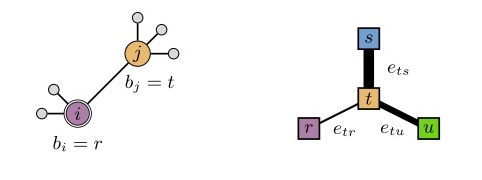
\includegraphics[width=0.9\linewidth]{pictures/topic/peixioto_move.jpg}
  \caption{Left: Local neighbourhood of node $i$ belonging to block $r$, and a randomly chosen neighbour $j$ \
  belonging to block $t$. \
  Right: Block multi-graph, indicating the number of edges between blocks, represented as the edge thickness. \
  In this example, the attempted move $bi \to s$ is made with a larger probability than either $bi \to u$\
   or $bi \to r$ (no movement), since $e_{ts}>e_{tu}$ and $e_{ts}>e_{tr}$.}
  \label{fig:topic_peixioto_move}
\end{figure}

In order to remove eventual biases due to the initial configuration the model is run with $5$ different initial states, then the final state with the minimal entropy is selected.

Once the model run it is possible to estimate the probability distribution of words inside a topic
\[P(w|t_w)=\frac{\text{\# of edges on $w$ to $t_w$}}{\text{\# of edges on $t_w$}}\]
and the topic distribution inside a document
\[P(t_w|d)=\frac{\text{\# of edges on $d$ from $t_w$}}{\text{\# of edges on $d$}}\]
This algorithm can set to have overlapping partitions; in this case, the presence of a word in a topic is not trivial and can be estimated as
\[P(t_w|w)=\frac{\text{\# of edges on $w$ to $t_w$}}{\text{\# of edges on $w$}}\]
or the presence of a document in a cluster
\[P(t_d|d)=\frac{\text{\# of edges on $d$ to $t_d$}}{\text{\# of edges on $d$}}\]

See appendix~\ref{app:hsbm} for a detailed analysis of the maths behind the algorithm and \url{https://cloud.docker.com/repository/docker/fvalle01/hsbm} for the extension of~\cite{gerlach2018network} to non-linguistics component systems datasets.


%%metrics
\section{Metrics and benchmarks}
Before running topic modelling, it is useful to define some metrics to test and benchmark the model. In particular the model searches sets on the two sides of the network the one containing samples and the one containing genes. Samples are extracted from datasets where much metadata are available, some of these metadata labels will be used to benchmark the model. To study genes enrichment test are necessary.

Looking at the samples side of the network, the outputs are sets of samples, the clusters. One can state the model works if all, or at least the majority, of samples in the same cluster share some label. Here the tissue is considered as the main label.

Note that this work's model is a non supervised one, but a ground truth is available from metadata. So every sample has a certain probability to have a certain property (the true tissue label), let's call this $P(C)$ and a certain probability of being in a cluster (model's output), let's call this $P(K)$.
It is possible to define some quantities, the homogeneity
\begin{equation}\label{eq:homogeneity}
    h=1-\frac{H(C|K)}{H(C)}
\end{equation}
defining the entropy
\begin{equation}\label{eq:hck}
    H(C|K)=\sum_{c\in \mathrm{tissues},\\ k \in \mathrm{clusters}}\frac{n_{c k}}{N}Log\left(\frac{n_{c k}}{n_k}\right)
\end{equation}
where $n_{c k}$ is the number of nodes of type $c$ in cluster $k$, $N$ the number of nodes and $n_k$ the number of nodes in cluster $k$. It is evident that if all nodes inside cluster $k$ are of the same type $c$ $n_{c k}=n_{k}$, $H(C|K)=0$ and $h=1$, it is actually a complete homogeneous situation.

Another quantity can be defined: the so-called completeness
\begin{equation}\label{eq:completness}
    c=1-\frac{H(K|C)}{H(K)},
\end{equation}
$H(K|C)$ is defined in the same way as~\ref{eq:hck}. Completeness measures how well nodes of the same type are distributed in the same cluster.

Ideally one wants a method which output is both homogeneous and complete. So it is possible to define the V-measure as the harmonic average of the two:
\begin{equation}\label{eq:mutualinformation}
    \mathrm{V-measure}=2\frac{h c}{h + c},
\end{equation}
which is actually the normalized mutual information between $P(C)$ and $P(K)$~\cite{rosenberg2007v}. Please refer to appendix~\ref{app:vmeasure} for the detailed maths. In figure~\ref{fig:topic/metric_scores_primarysite} an example of the V-measure score estimated at the different layers of the hierarchy; note that the number of clusters increases going deeper in the hierarchy. In the same figure homogeneity and completeness are reported, note that with few clusters the situation is more complete, but when the number of clusters increases completeness goes down and homogeneity increases. 
\begin{figure}[htb!]
    \centering
    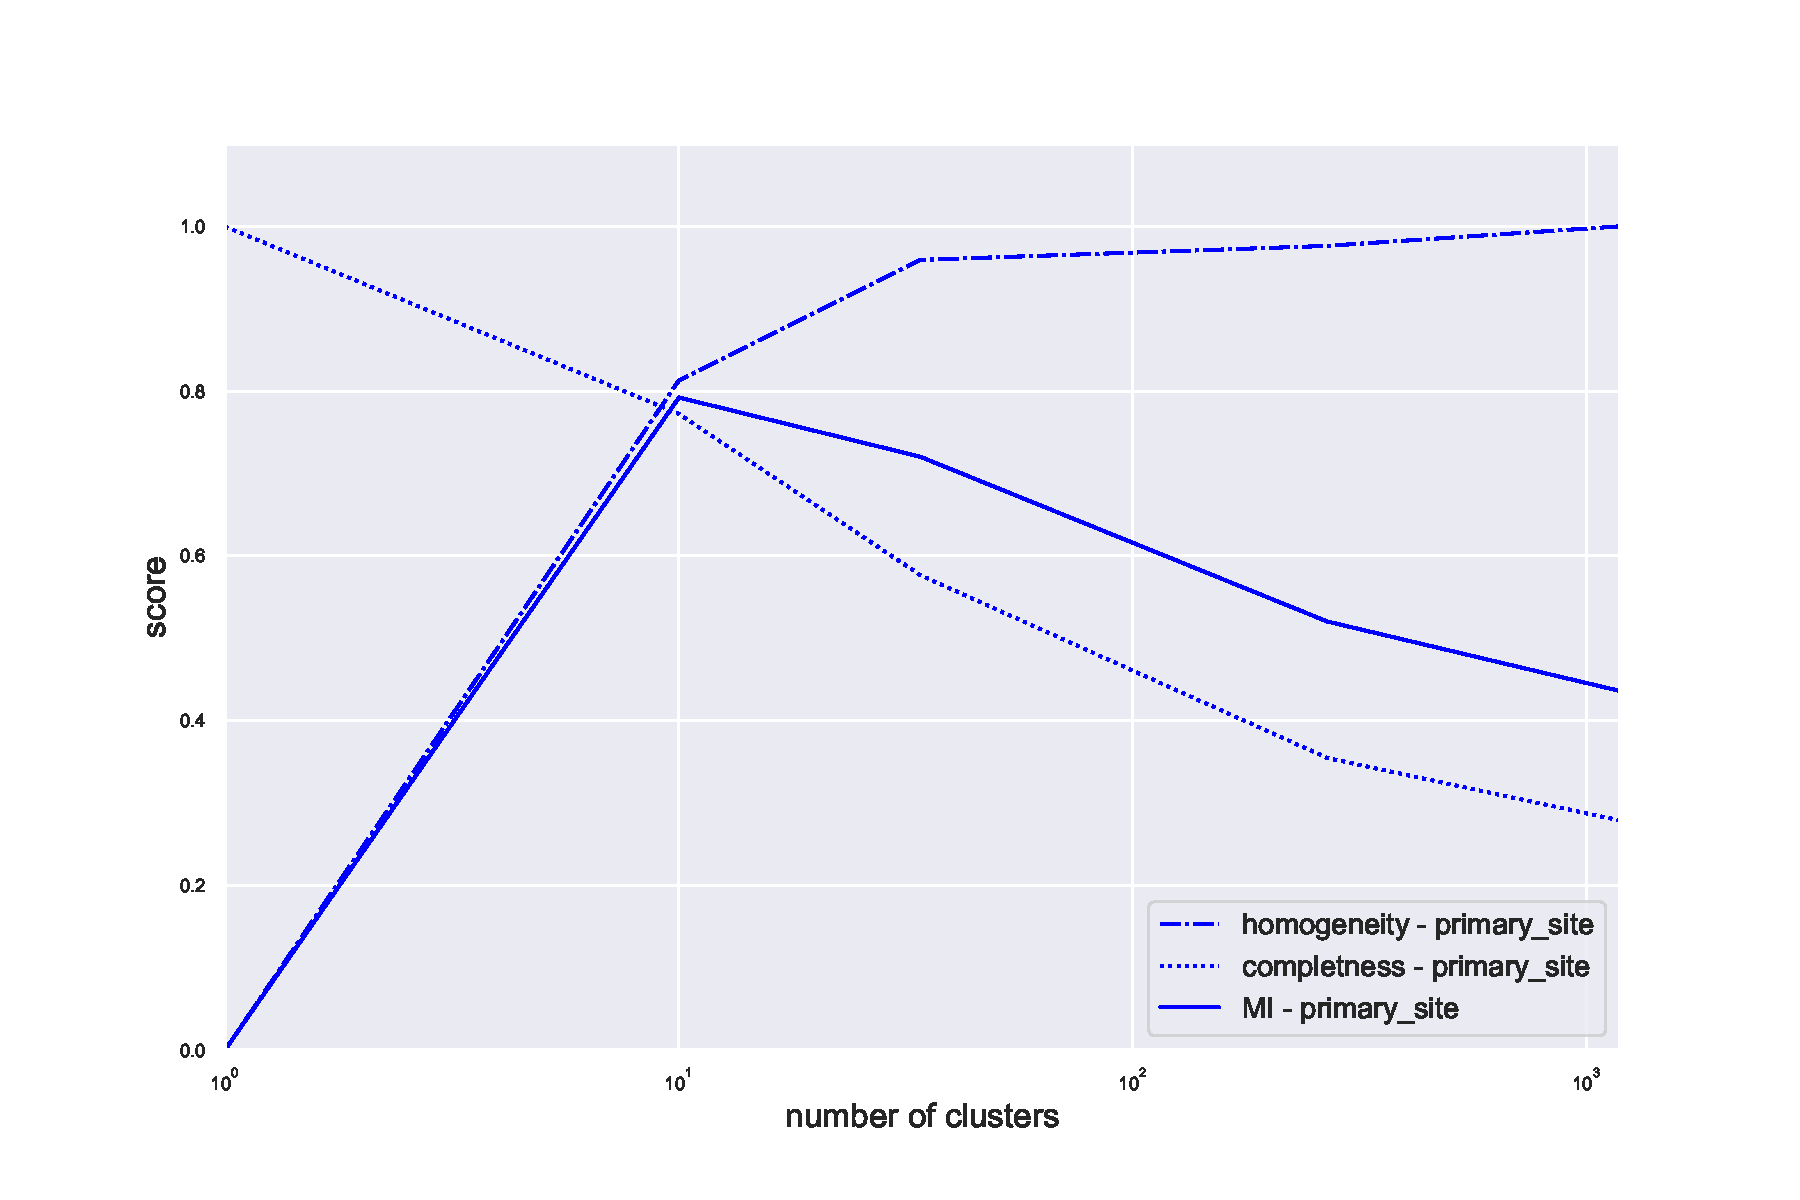
\includegraphics[width=0.8\linewidth]{pictures/topic/gtex/oversigma_10tissue/metric_scores_primarysite.pdf}
    \caption{Score across hierarchy. The V-measure or normalized mutual information MI is the harmonic average between homogeneity and completeness.}
    \label{fig:topic/metric_scores_primarysite}
\end{figure}

In the next sections will be studied also the maximum fraction of label in the same cluster defined as 
\[\mathrm{max}_{c\in k}\frac{n_{c k}}{n_k}.\] Also the number of different labels in the same cluster will be studied.
\FloatBarrier

%%comparables algorithms
\subsection{LDA}
\draft{commenti vari}

As in ~\cite{Zhou2016}
\begin{equation}\label{eq:lda}
  P(w, z,\beta, \theta| \alpha, \eta)=\prod_n^{N_d} P(w|z,\beta)P(z|\theta)\prod_k^KP(\beta|\eta)\prod_d^N P(\theta | \alpha)
\end{equation}

\begin{figure}
  \centering
  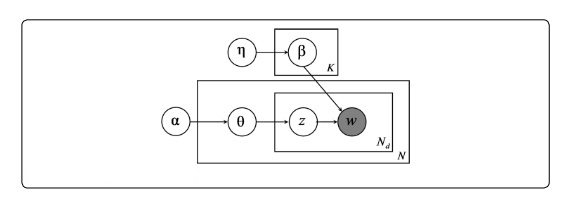
\includegraphics[width=0.5\linewidth]{pictures/topic/LDA.jpeg}
  \label{fig:LDA}
  \caption{LAD scheme}
\end{figure}
where
\begin{itemize}
  \item $N$ number of documents
  \item $K$ number of topics
  \item $w$ words
  \item $N_d$ number of words in document d
  \item $\eta$ and $\alpha$ are parameters of the model
\end{itemize}
in~\ref{eq:lda} $P(\theta | \alpha)$ and $P(\beta|\eta)$ are Dirichlet distributions the outputs are the topic distribution in documents $P(z|d)$ and the word distribution in topics $P(w|z)$

\subsection{Hierarchical clustering}

\draft{da scrivere}

\draft{hierarchical clustering}
Hierarchical clustering is a general family of clustering algorithms that build nested clusters by merging or splitting them successively. This hierarchy of clusters is represented as a tree (or dendrogram). The root of the tree is the unique cluster that gathers all the samples, the leaves being the clusters with only one sample. See the Wikipedia page for more details.

The AgglomerativeClustering object performs a hierarchical clustering using a bottom up approach: each observation starts in its own cluster, and clusters are successively merged together. The linkage criteria determines the metric used for the merge strategy:

Ward minimizes the sum of squared differences within all clusters. It is a variance-minimizing approach and in this sense is similar to the k-means objective function but tackled with an agglomerative hierarchical approach.
Maximum or complete linkage minimizes the maximum distance between observations of pairs of clusters.
Average linkage minimizes the average of the distances between all observations of pairs of clusters.
Single linkage minimizes the distance between the closest observations of pairs of clusters.
AgglomerativeClustering can also scale to large number of samples when it is used jointly with a connectivity matrix, but is computationally expensive when no connectivity constraints are added between samples: it considers at each step all the possible merges.


\begin{lstlisting}[style=mypython]
from sklearn.cluster import AgglomerativeClustering
AgglomerativeClustering(
    affinity='euclidean',
    compute_full_tree='auto',
    linkage='ward',
    n_clusters=x,
    )
\end{lstlisting}



%%preprocess
\section{Pre-process}
To make the algorithm faster, it could be useful to do a pre-processing of the data.
Different approaches were tested, all of them involving the quantities defined in~\ref{ch:structure}. The goal is to identify components which are able to best separate the realizations. 
\paragraph{Low occurrence genes} were selected firstly to approach topic modelling. A $0.5$ threshold was set on occurrence. This method selects genes that appears (have expression greater than zero) only in less than half samples. This approach has some limitations, for instance it doesn't consider genes that appear everywhere (with occurrence $\simeq 1$) but changes their behaviour across realisations.

\paragraph{tf-idf (term frequency–inverse document frequency)} should help. This approach doesn't take in account original expression values $n_{ij}$, but a transformed version
\[
n^{new}_{ij}=\frac{n_{i j}}{M_j}\times \left(1-Log\left(o_i\right)\right)
\] which increases the importance of components with small occurrence $o_i$. This approach doesn't actually select components, which is still an issue.

\paragraph{Highly variable} genes can be selected. This is done using the $CV^2$ analysis done in chapter~\ref{ch:scalinglaws}.
\begin{figure}[htb!]
    \centering
    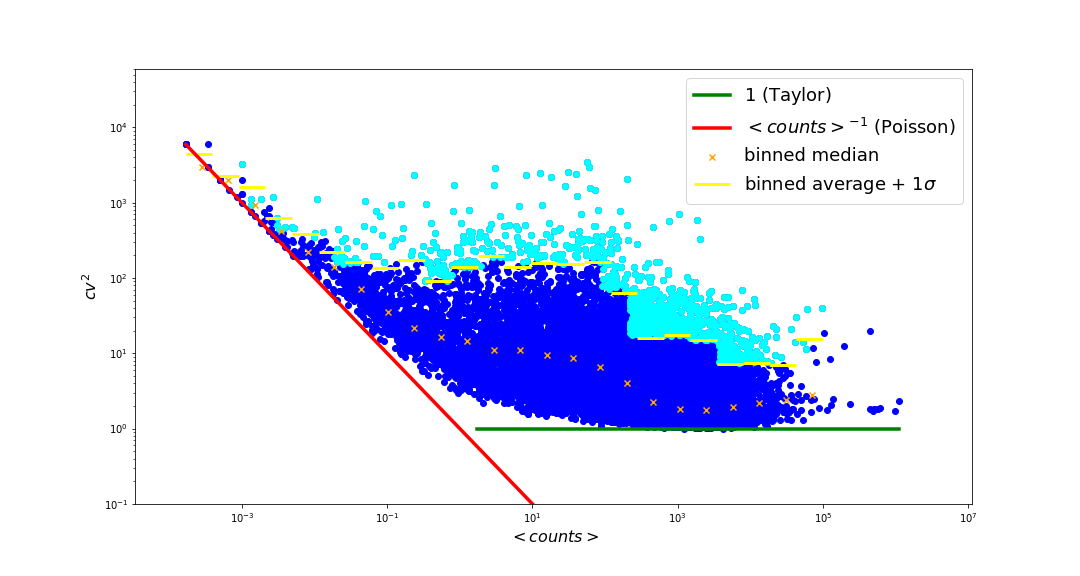
\includegraphics[width=0.8\linewidth]{pictures/topic/cvmean_oversigma.png}
    \caption{Highly variable genes}
    \label{fig:topic/cvmean_oversigma}
\end{figure}
Plotting the coefficient of variation versus the mean for each component reveals which components have higher variance with respect to components which, on average, have a similar behaviour. Binned averages and variances were estimated, and only genes with a $CV^2$ over a $\sigma$ greater than the bin's mean were considered. This method seems to select useful genes even if the binned average bound is quite noisy.

\paragraph{Distance from boundaries} can be a similar and alternative method to select highly variable genes. In this case the bound is smooth and well defined.
\begin{figure}[htb!]
    \centering
    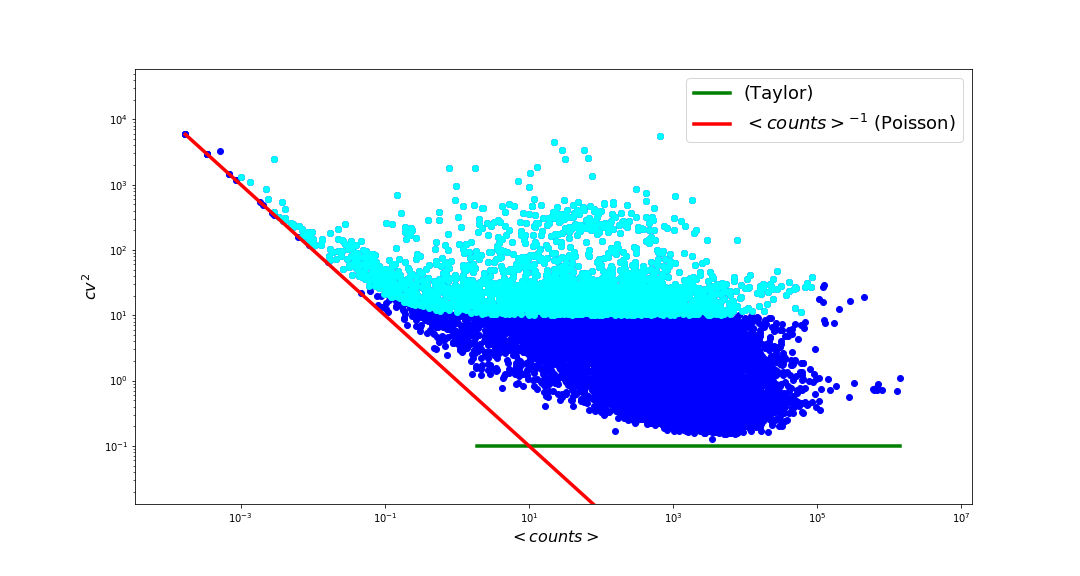
\includegraphics[width=0.8\linewidth]{pictures/topic/cvmean_oversampling.png}
    \caption{Genes distant from the boundaries}
    \label{fig:topic/cvmean_oversampling}
\end{figure}
The distribution as discussed in~\ref{ch:scalinglaws} have a Poisson-like and a Taylor-like boundaries. So can be considered only components that are the most distant from these boundaries. Moreover this boundaries can be found with a simple null model, as shown in figure~\ref{fig:scaling/gtex/cvmean_loglog_sampling} the sampling model defines the lower bound of the data.

The last two approaches are the ones which lead to better results, in the following sections gene selection was done by getting only highly variables genes.

\clearpage
\section{Run}\label{sec:run}
%%gtex
\subsection{Run on Gene Tissues Expression dataset}
Once the model was set and adapted to RNA-Sequencing data, it was run on a subset of the GTEx dataset. A subset of samples was chosen randomly to reduce the computing time needed. The analysis hereby described took about 2 days to be run on a 16 core CPU, 100GB memory facility. The great amount of memory is needed to temporary store the network configuration at each step of the Monte Carlo simulation.

First of all, to rapidly have information about the interest of the oncoming result the metric above described were considered. In figure~\ref{fig:topic/gtex/oversigma_10tissue/metric_scores} it is represented the V-measure score versus the number of clusters found at different layers.
\begin{figure}[htb!]
    \centering
    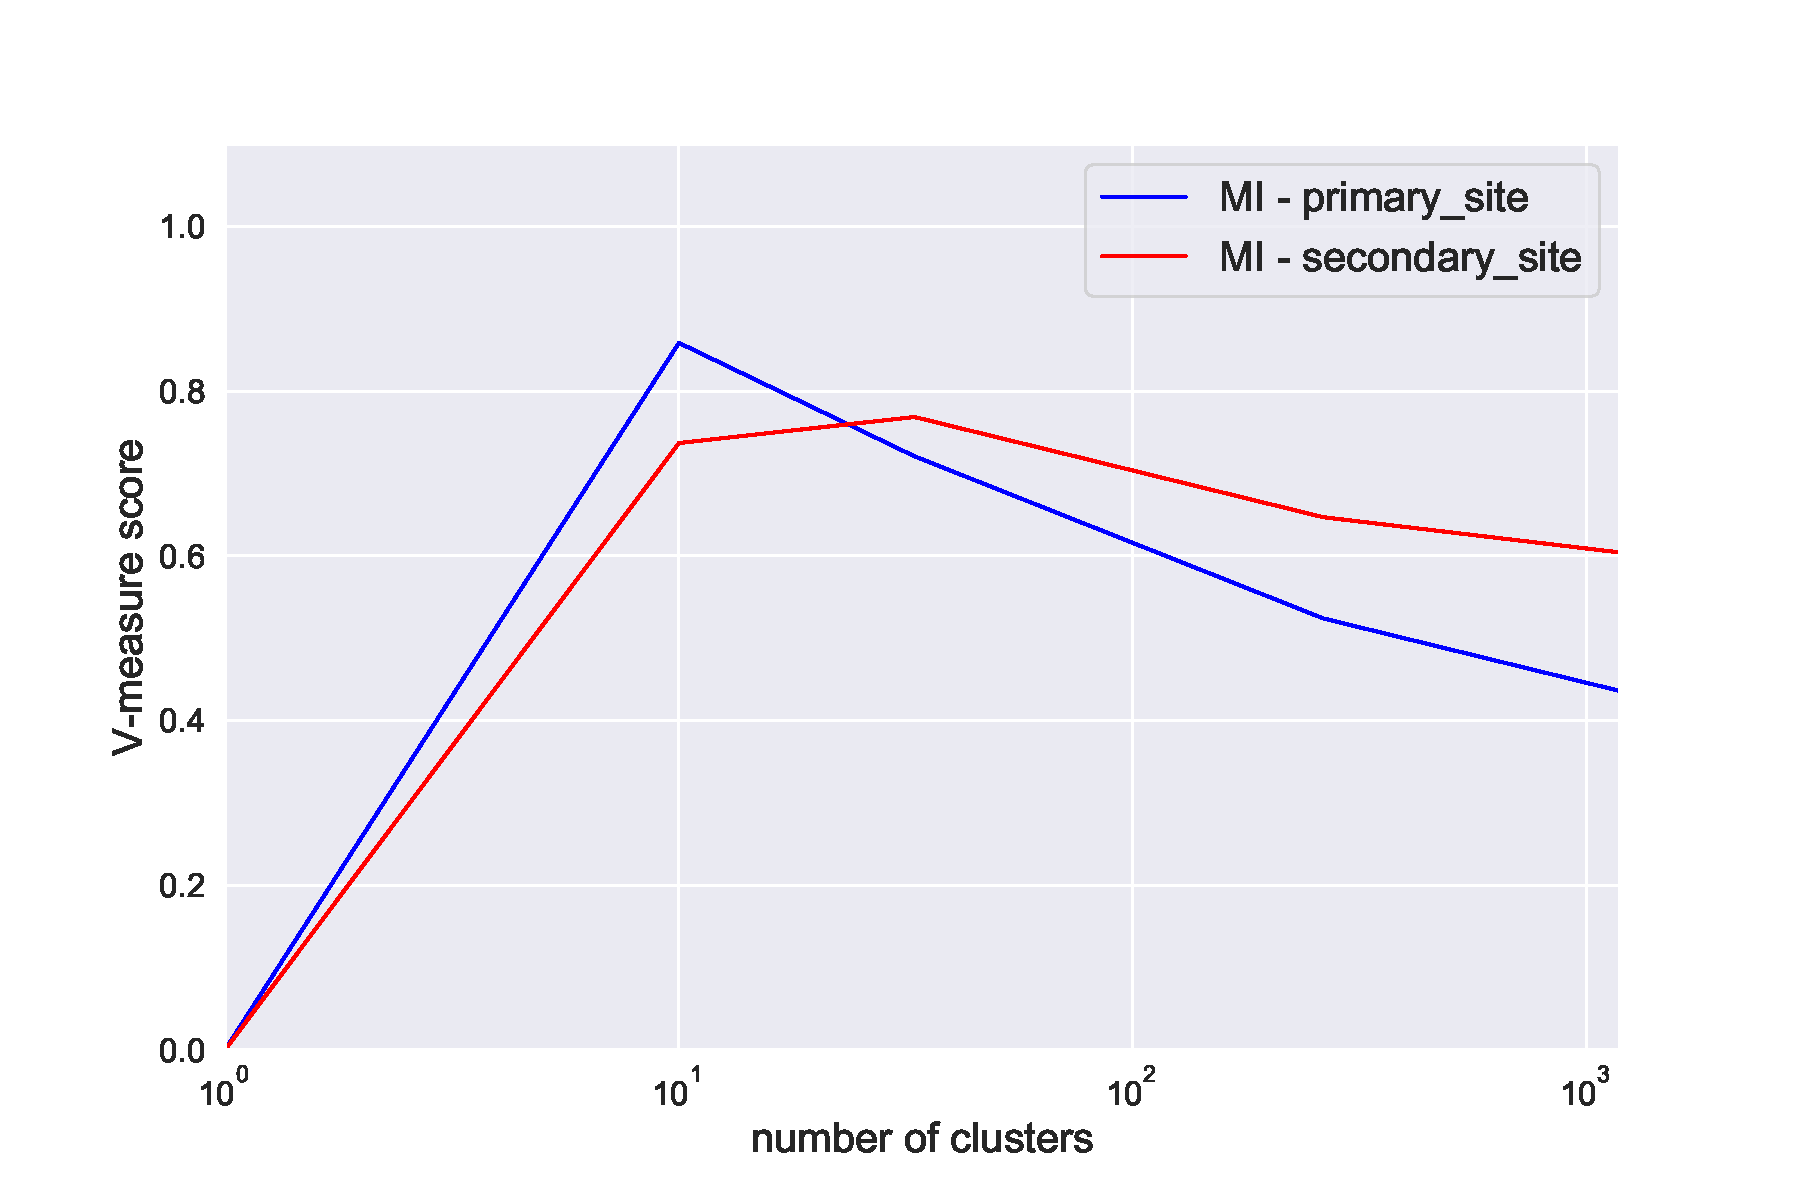
\includegraphics[width=0.9\linewidth]{pictures/topic/gtex/oversigma_10tissue/metric_scores.pdf}
    \caption{Scores across the hierarchy. The performances classifying the primary site and secondary site are compared. Note that with one cluster the completeness is $1$ but the homogeneity is $0$ so the score goes down.}
    \label{fig:topic/gtex/oversigma_10tissue/metric_scores}
\end{figure}
The result is quite good, the maximum score is over $0.8$. Considering that, for example,~\cite{Farver2018} obtained a similar score analysing similar dataset considering just homogeneity, this can be considered a quite good result. A second interesting fact is that both the tissue label (primary site) and the sub-tissue label (secondary site) obtain such a good score. Moreover, the secondary site score's peak is at a higher number of clusters coherently with the fact that there is a greater number of sub-tissue labels. This score can be useful to extract the correct level of the hierarchy the consequent analysis should be made on.

In figure~\ref{fig:topic/gtex/oversigma_10tissue/bipartite_rebuild} the relationship between the clusters at different layers is evident. Each row is a layer of the hierarchy and arrows represent the path of a node across the hierarchy. Note that clusters don't overlap and the separation done at the greater level is maintained across all the hierarchy. This representation gives an idea of the point of the hierarchy where the tissues separate, see in figure~\ref{fig:topic/gtex/oversigma_10tissue/bipartite_rebuild} cluster $2$ that splits in two clusters separating \textit{breast} and \textit{adipose tissue}.
\begin{figure}[htb!]
    \centering
    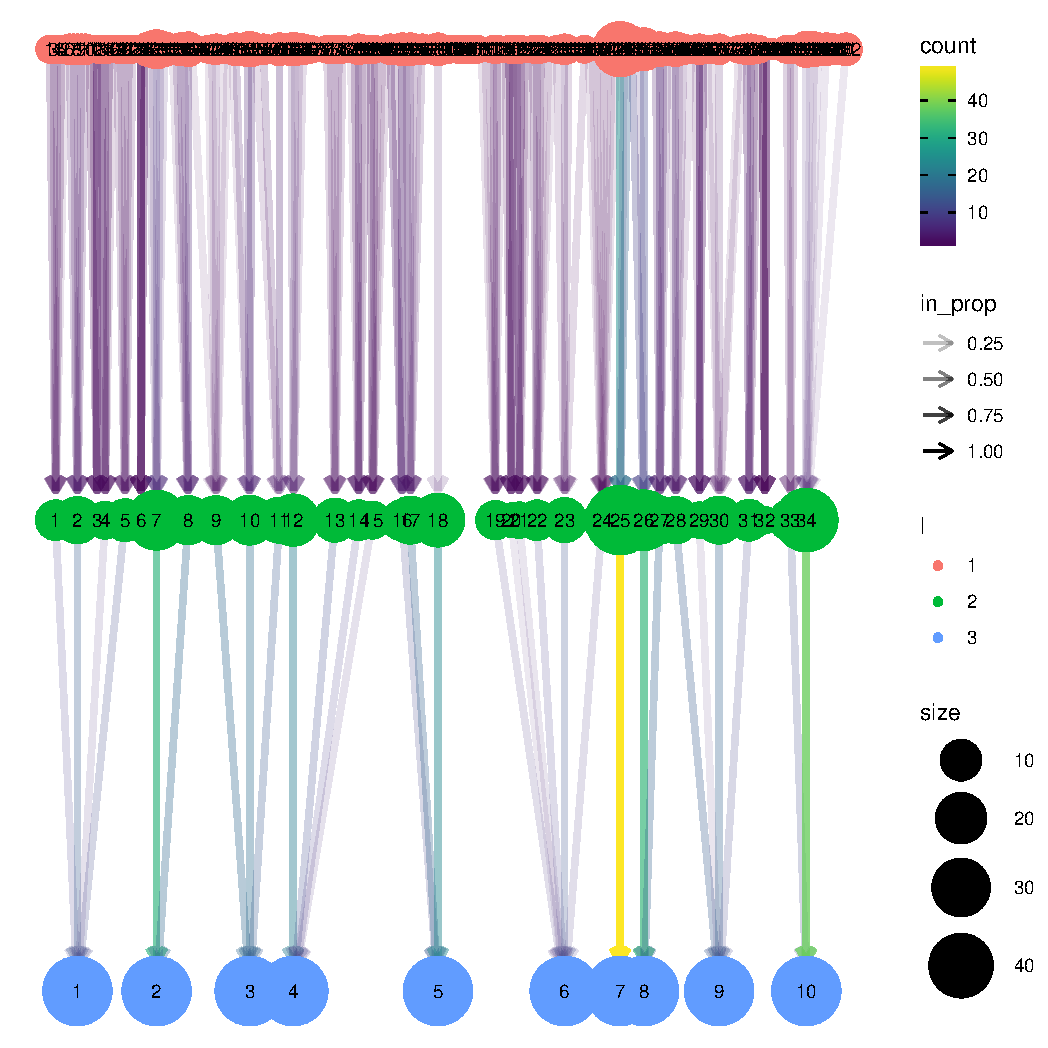
\includegraphics[width=0.8\linewidth]{pictures/topic/gtex/oversigma_10tissue/bipartite_rebuild.pdf}
    \caption{Hierarchy of the files' nodes. In the top the layers where the output consists of many small clusters, in the bottom the output with few big clusters. Arrows represent how nodes pass from a hierarchy layer to another. The bigger the balls, the bigger the cluster. The more yellow the link the more nodes are in common between the clusters of the two different layers. Plotted using clustree~\cite{clustree}.}
    \label{fig:topic/gtex/oversigma_10tissue/bipartite_rebuild}
\end{figure}

\clearpage
In figure~\ref{fig:topic/gtex/oversigma_10tissue/clustercomposition_l3_primary_site} each column is a cluster and each colour is a tissue of the dataset. It is evident that the majority of the tissues are identified: the first, second, fourth, fifth, sixth, seventh, and tenth columns are fully and uniformly coloured of the same colour. These correspond to an identification of \textit{brain}, \textit{skin}, \textit{lung}, \textit{blood} and \textit{testis}.
\begin{figure}[htb!]
    \centering
    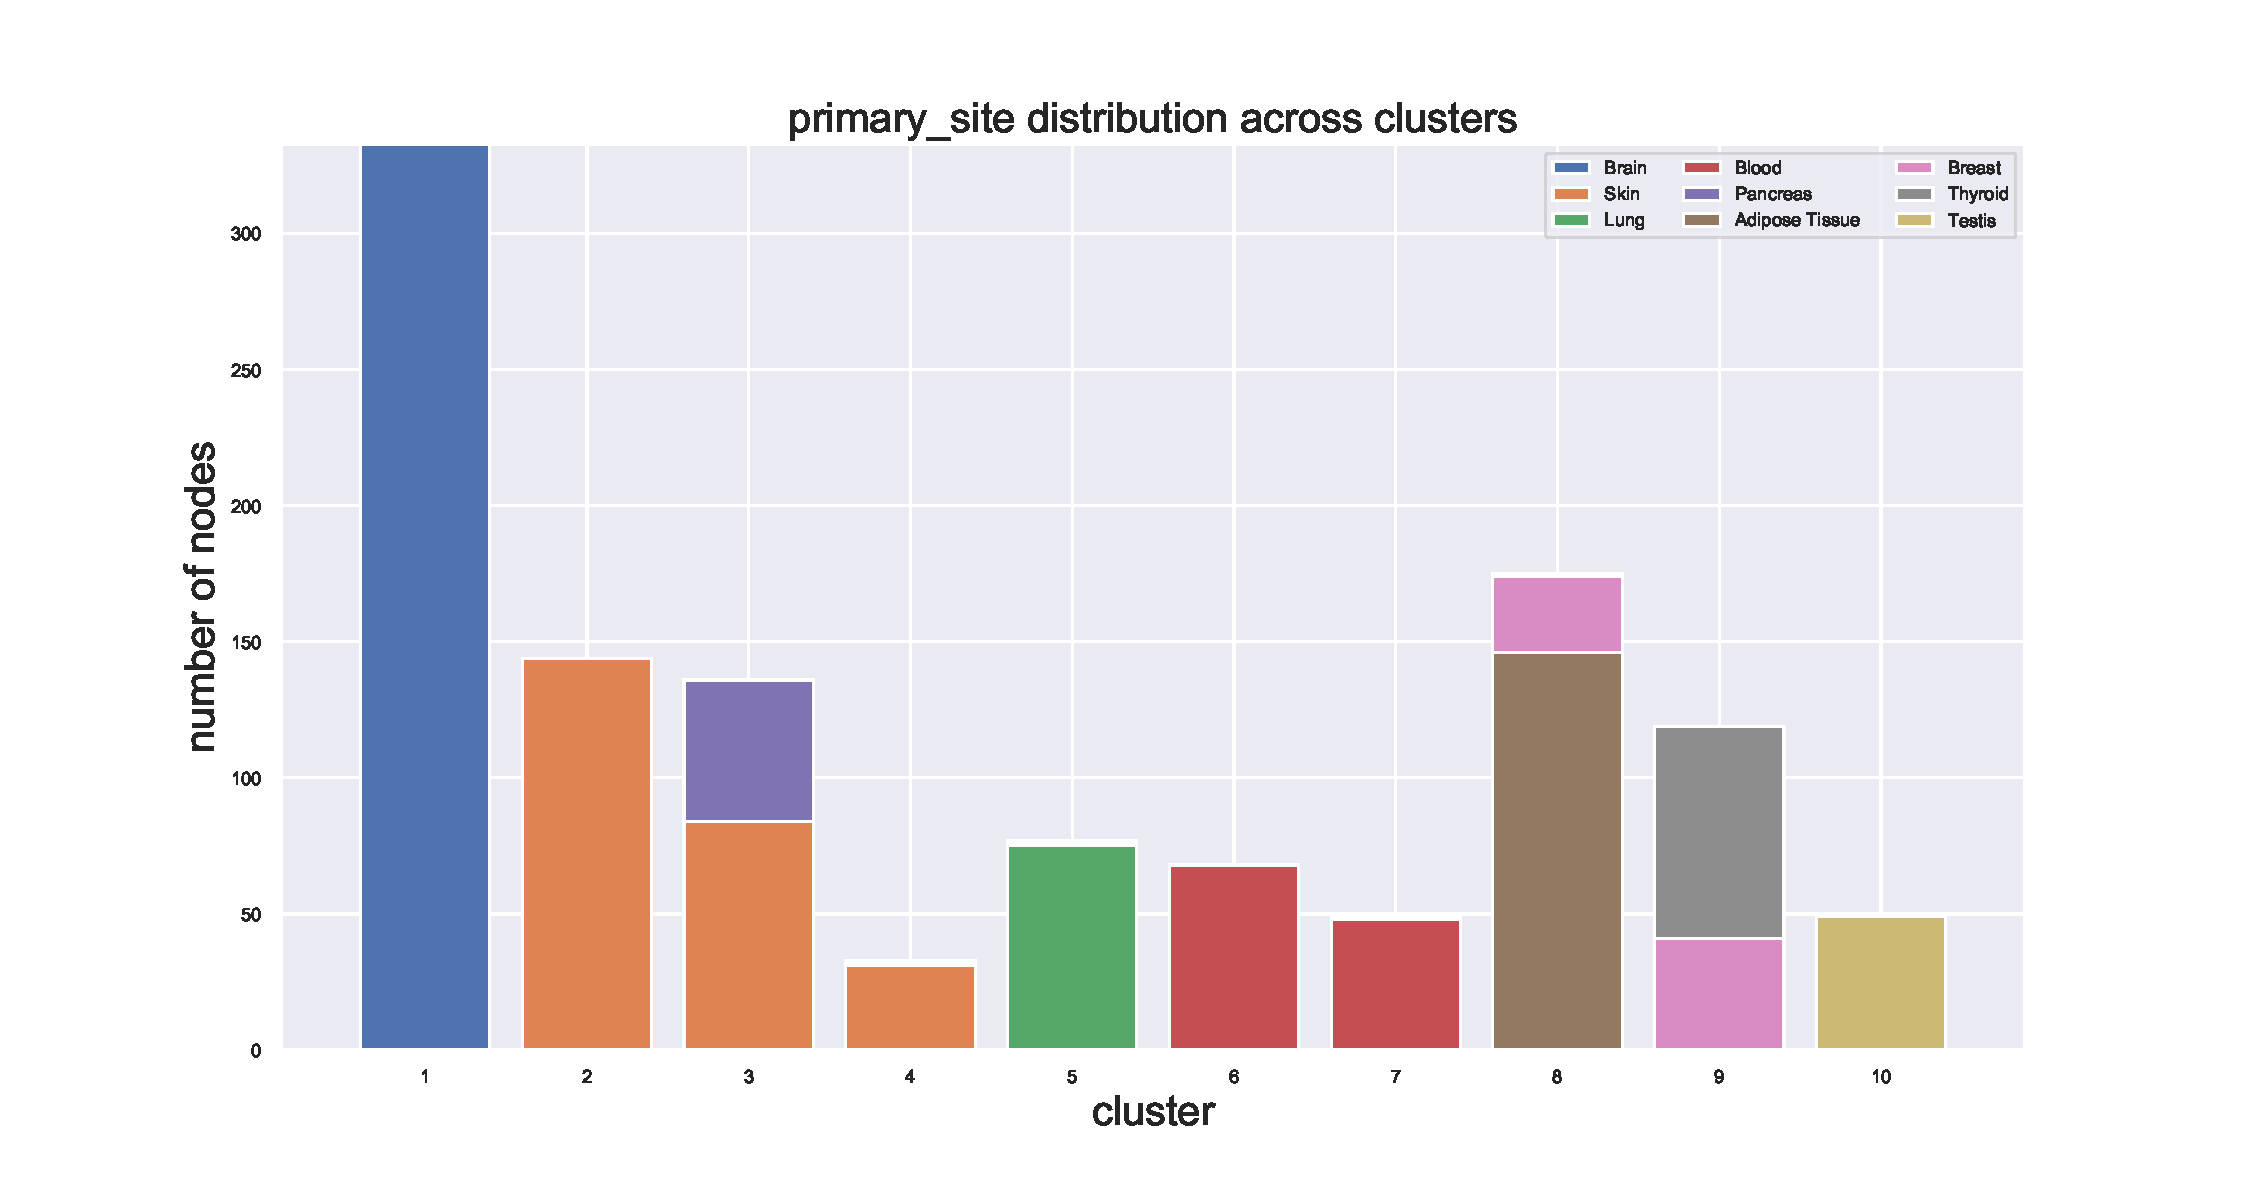
\includegraphics[width=0.9\linewidth]{pictures/topic/gtex/oversigma_10tissue/clustercomposition_l3_primary_site.pdf}
    \caption{Clusters composition at the level of the hierarchy with the higher score. Each column is a cluster, each colour is a label.}
    \label{fig:topic/gtex/oversigma_10tissue/clustercomposition_l3_primary_site}
\end{figure}
In the normalized representation of the same clusters the homogeneity of the clusters is more evident.
\begin{figure}[htb!]
    \centering
    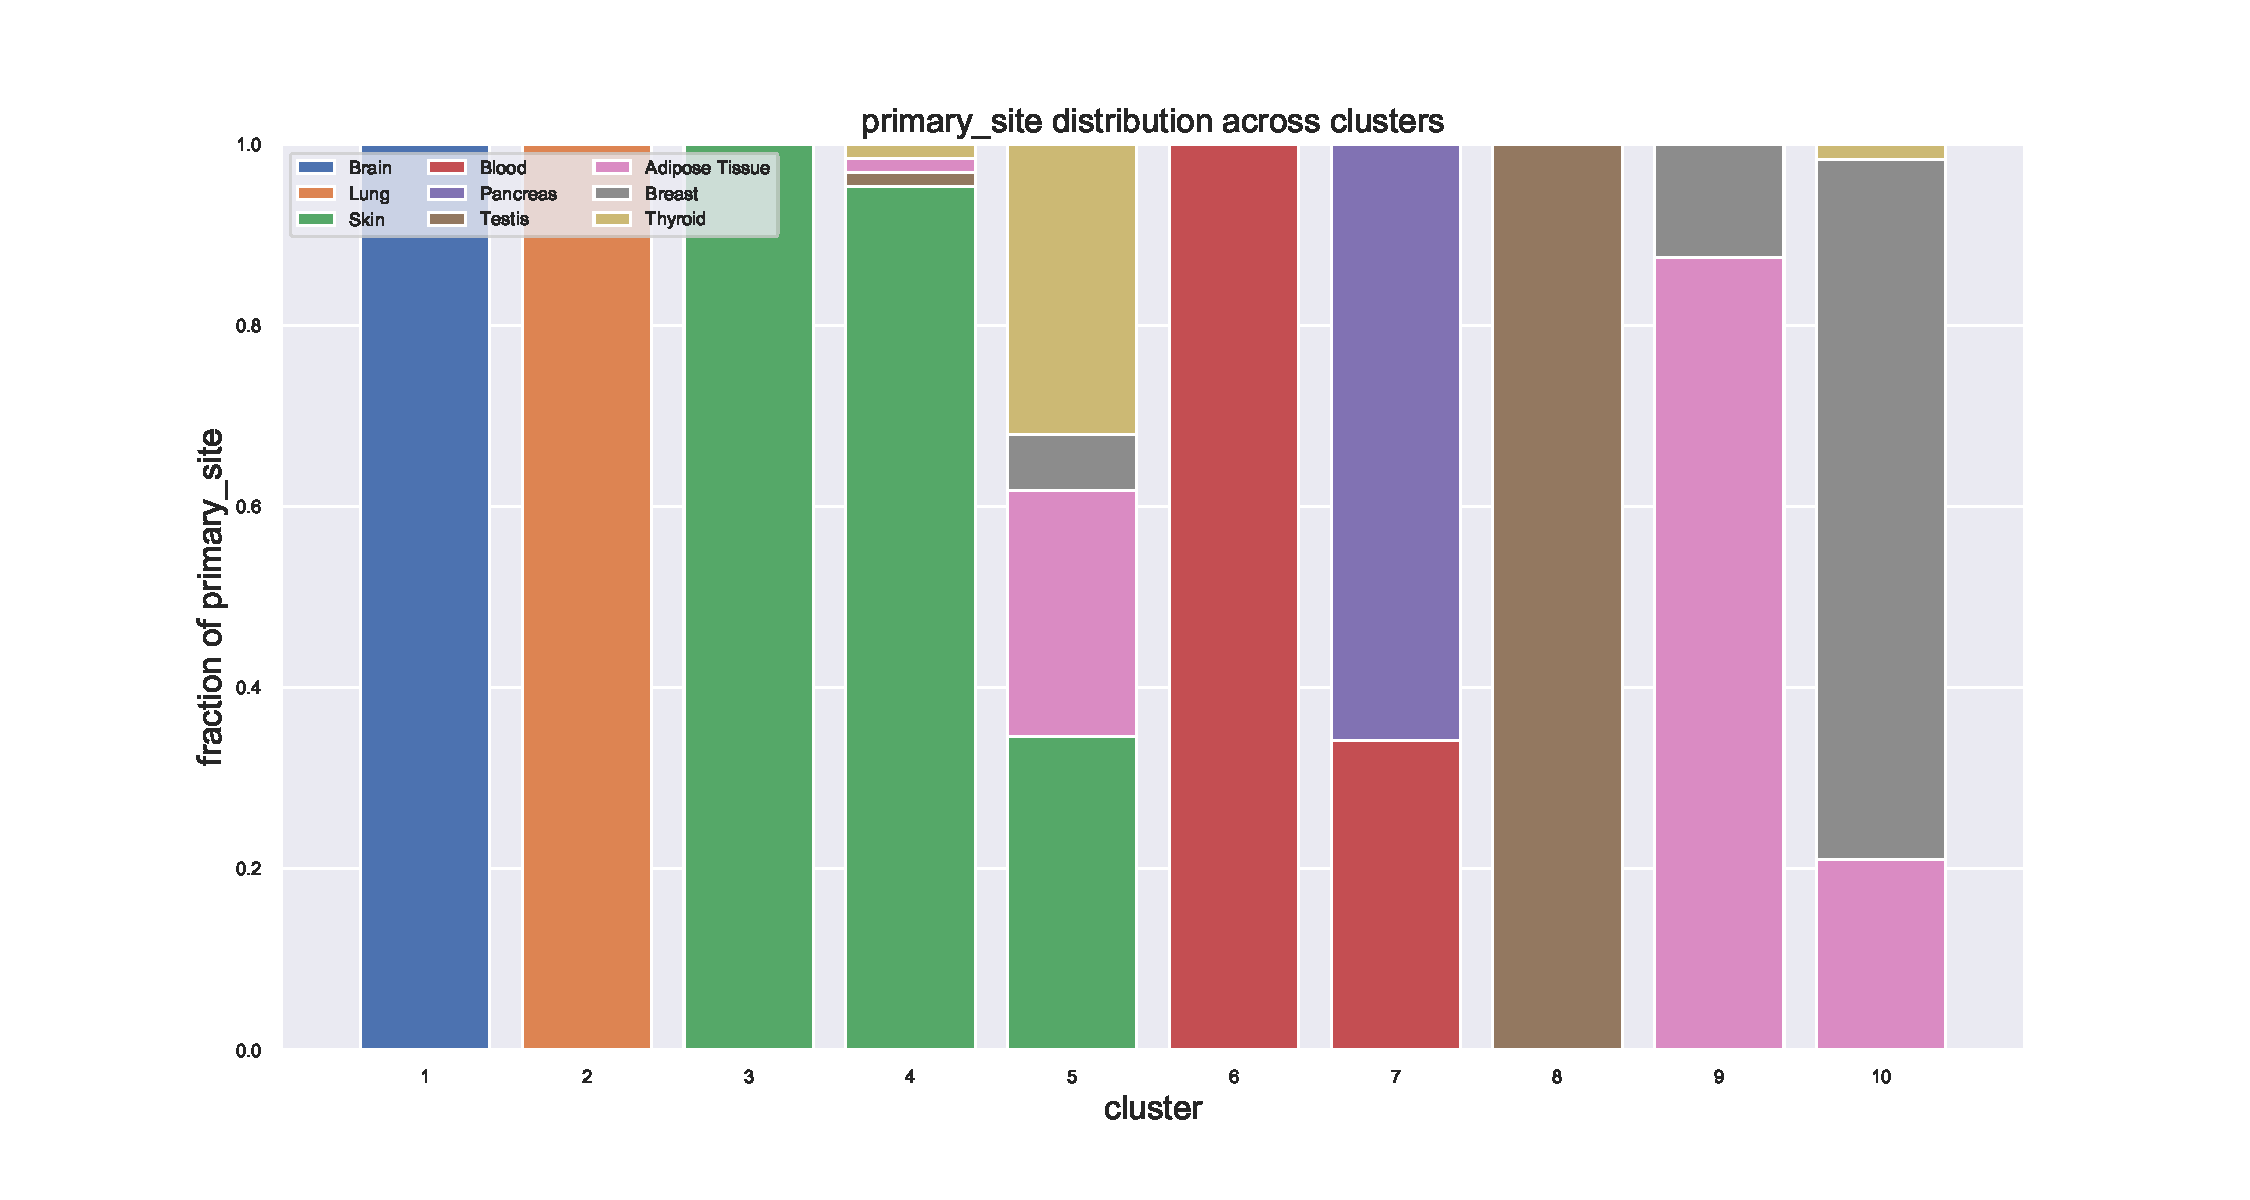
\includegraphics[width=0.9\linewidth]{pictures/topic/gtex/oversigma_10tissue/fraction_clustercomposition_l3_primary_site.pdf}
    \caption{Normalized composition of clusters. Again each column is a cluster, each colour is a label.}
    \label{fig:topic/gtex/oversigma_10tissue/fraction_clustercomposition_l3_primary_site}
\end{figure}
Going deeper in the hierarchy and looking at a layer with more cluster the result, shown in figure~\ref{fig:topic/gtex/oversigma_10tissue/fraction_clustercomposition_l2_primary_site}, demonstrates that, at this point, all the tissues are separated and each cluster is full of nodes sharing the same tissue.
\begin{figure}[htb!]
    \centering
    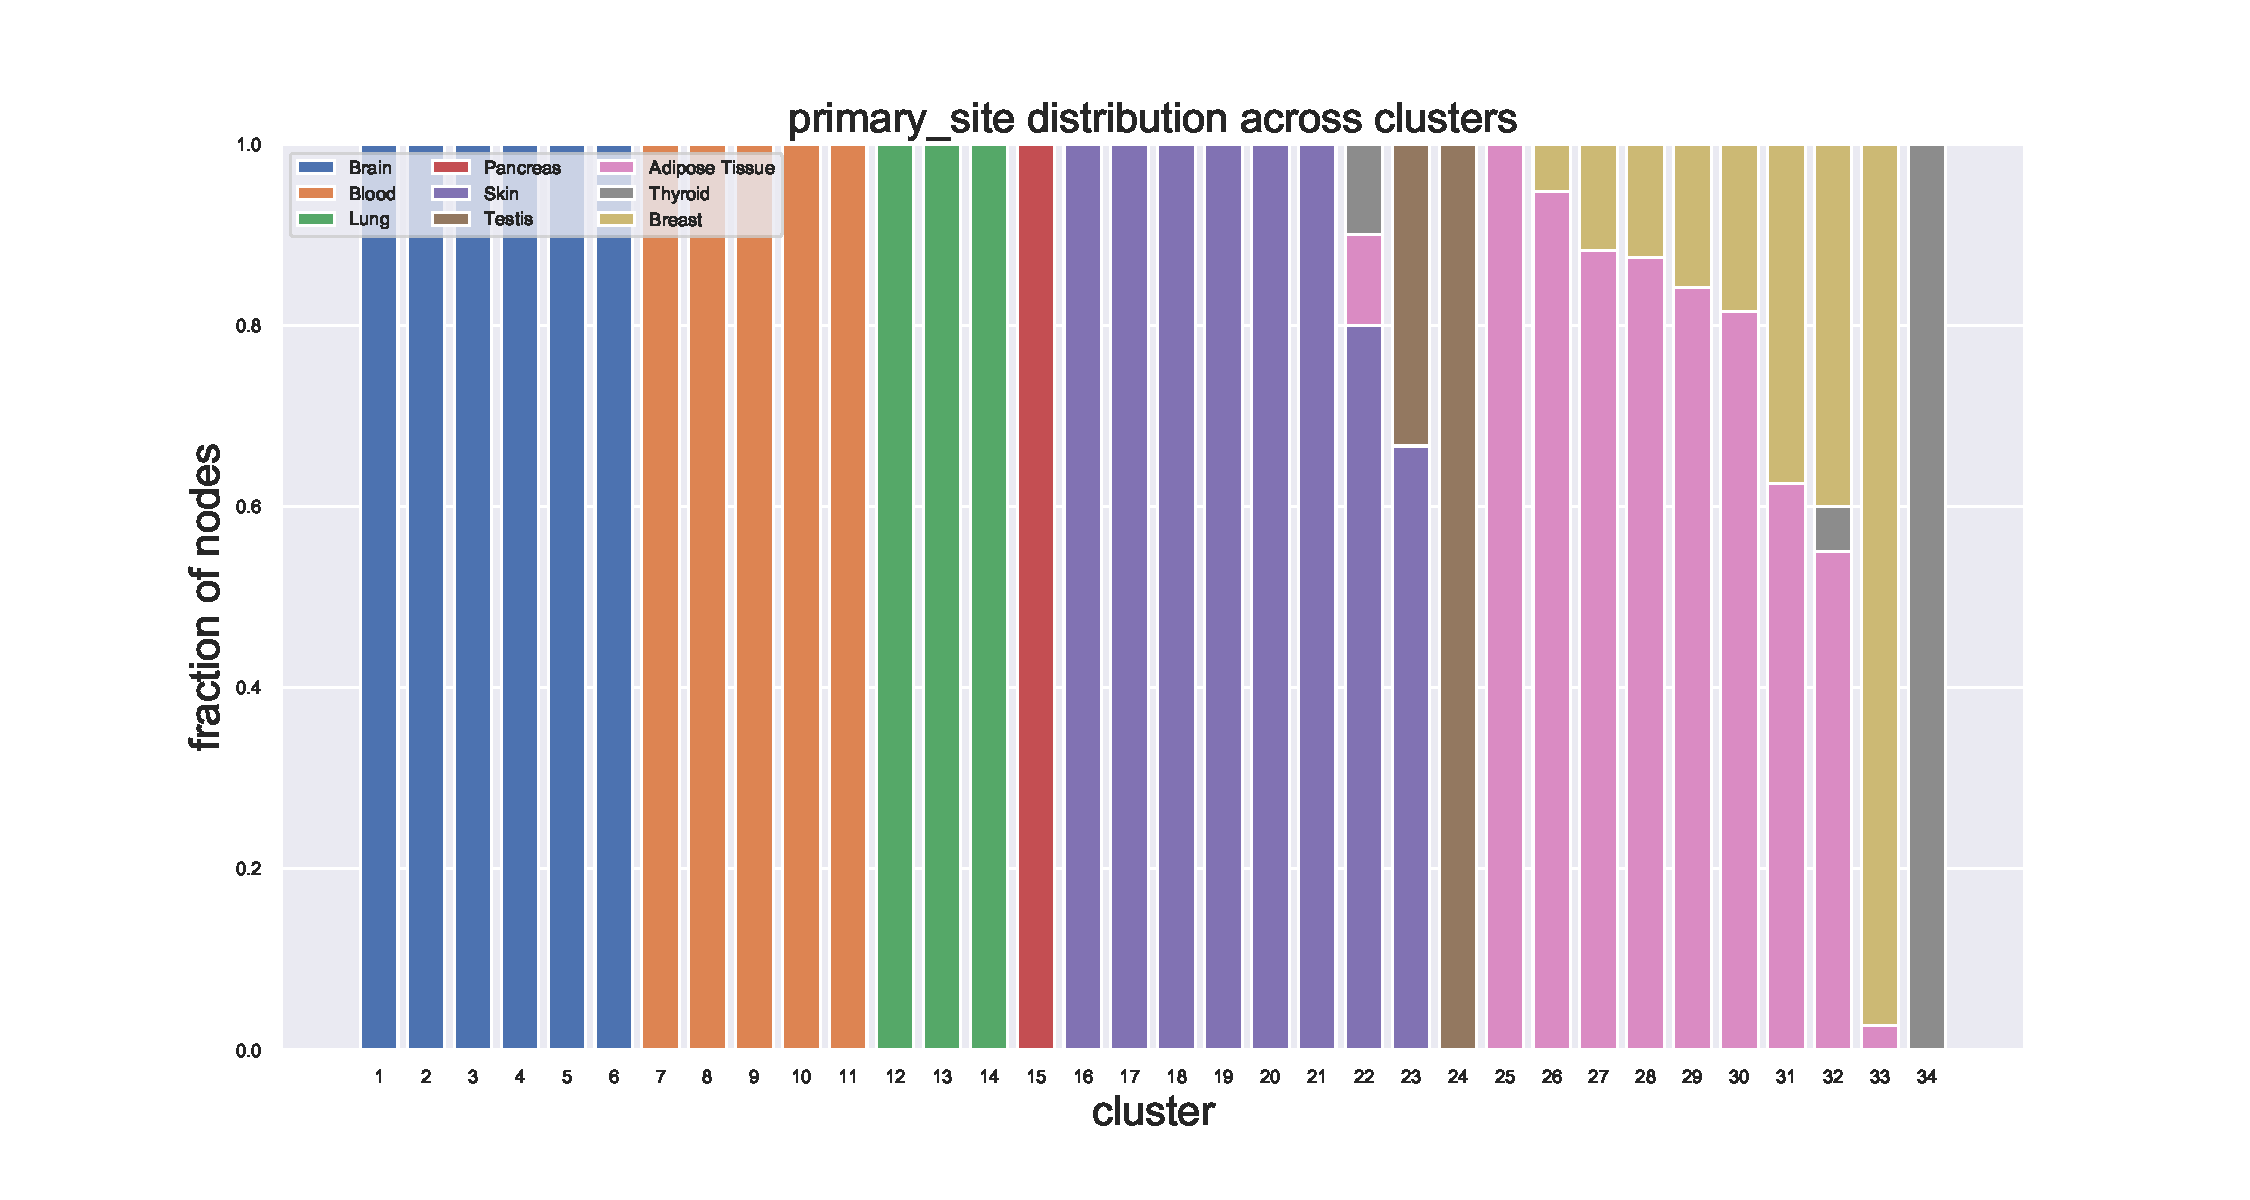
\includegraphics[width=0.9\linewidth]{pictures/topic/gtex/oversigma_10tissue/fraction_clustercomposition_l2_primary_site.pdf}
    \caption{Normalized composition of clusters at a deeper level.}
    \label{fig:topic/gtex/oversigma_10tissue/fraction_clustercomposition_l2_primary_site}
\end{figure}
Even looking at sub-tissues the results is quite good. It is not always easy to separate all the sub-parts of the \textit{brain}, nevertheless, the \textit{cerebellum} is well identified (column 27) and \textit{blood} is distinguished in \textit{whole blood} (columns 4-8) and \textit{lymphocytes} (column 3).
\begin{figure}[htb!]
    \centering
    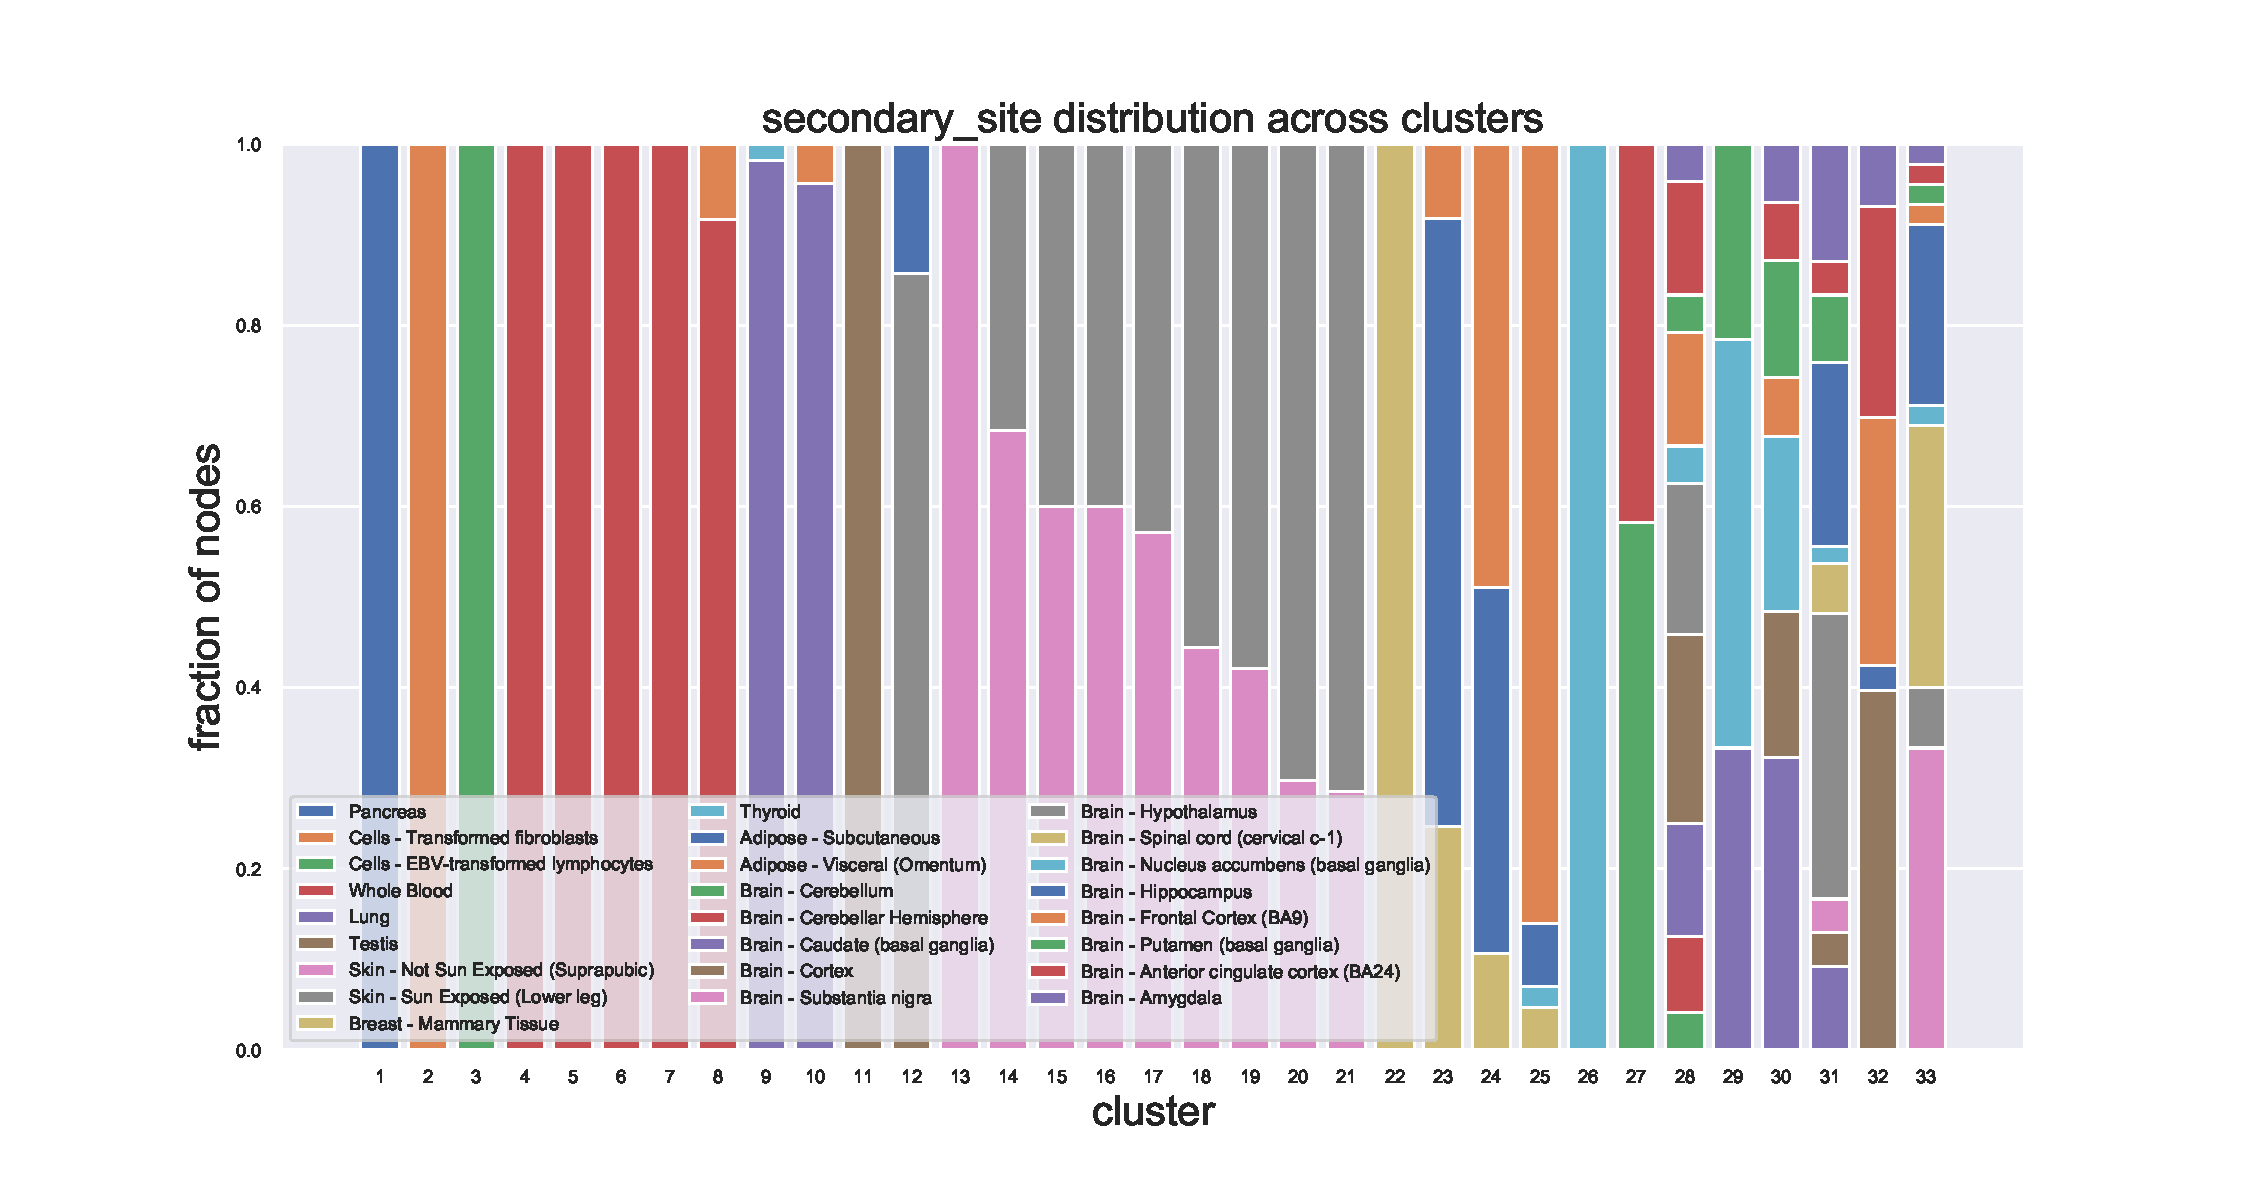
\includegraphics[width=0.9\linewidth]{pictures/topic/gtex/oversigma_10tissue/fraction_clustercomposition_l2_secondary_site.pdf}
    \caption{Normalized composition of clusters for the secondary site sub-tissue labels.}
    \label{fig:topic/gtex/oversigma_10tissue/fraction_clustercomposition_l2_secondary_site}
\end{figure}

\subsection{Null model shuffling labels}
A null model of cluster composition is necessary if one would be able to state that a result is better than expected. This was done by doing the same analysis but reshuffling the labels of the nodes. Reshuffling was done exchanging the label of each node with the one of another node picked up uniformly random. Doing so the number of clusters and the cluster sizes are maintained. In figure~\ref{fig:topic/gtex/oversigma_10tissue/shuffledclustercomposition_l3_primary_site} an example of clustering with random labels, it is evident that all clusters have similar and homogeneous composition. Note that not every tissue has the same number of samples, so, for example, \textit{brain} is more represented than other tissues.
\begin{figure}[htb!]
	\centering
	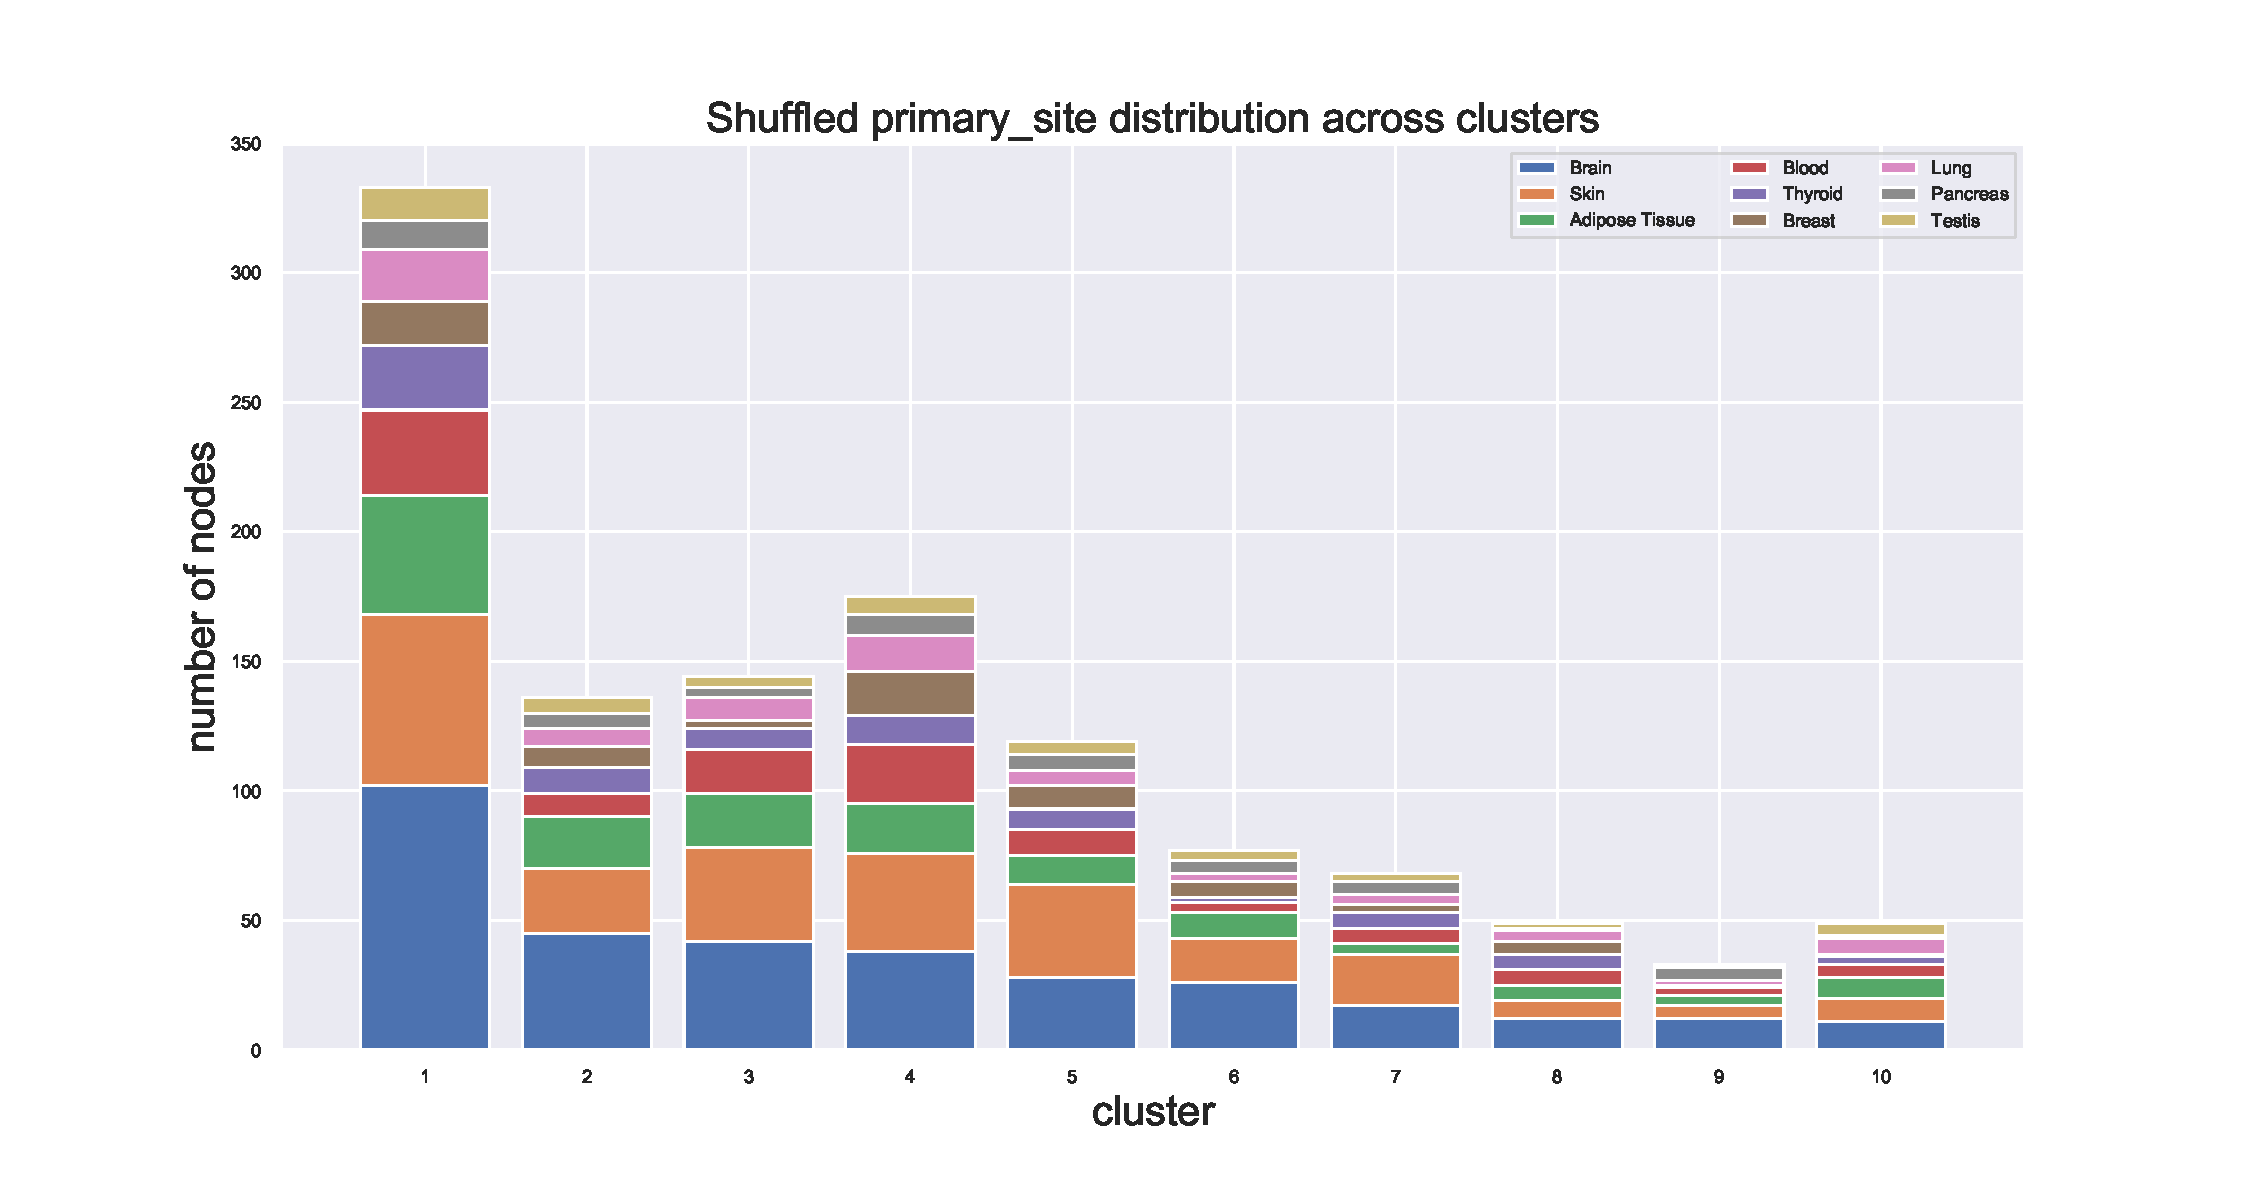
\includegraphics[width=0.9\linewidth]{pictures/topic/gtex/oversigma_10tissue/shuffledclustercomposition_l3_primary_site}
	\caption{Example of visualization of clusters with reshuffled labels.}
	\label{fig:topic/gtex/oversigma_10tissue/shuffledclustercomposition_l3_primary_site}
\end{figure}

All the results described in the previous pictures are quite qualitative. To have a more objective and mathematical measure of the success of the algorithm it is possible to measure the fraction of the most representative label in each cluster $k$
\[
max_{l\in labels}\left(\frac{n_{l k}}{n_k}\right)
\]
being $n_{l k}$ the number of nodes labelled $l$ in cluster $k$ and $n_k$ is the number of nodes in cluster $k$. This is represented in figure~\ref{fig:gtex/oversigma_10tissue/shuffledcluster_maximum_l2_primary_site} for the level where the V-measure is maximized (the best results are expected at this resolution). In figure~\ref{fig:gtex/oversigma_10tissue/shuffledcluster_maximum_l2_primary_site} on the left is shown the most representative label fraction for each cluster, on the right the histograms of the same quantity. Models' clusters are very homogeneous with the majority of cluster full, almost $100\%$, of the same tissue. It is also clear that reshuffling the labels the result is very different and so it is possible to admit that the models behave better than expected. 
\begin{figure}[htb!]
    \centering
    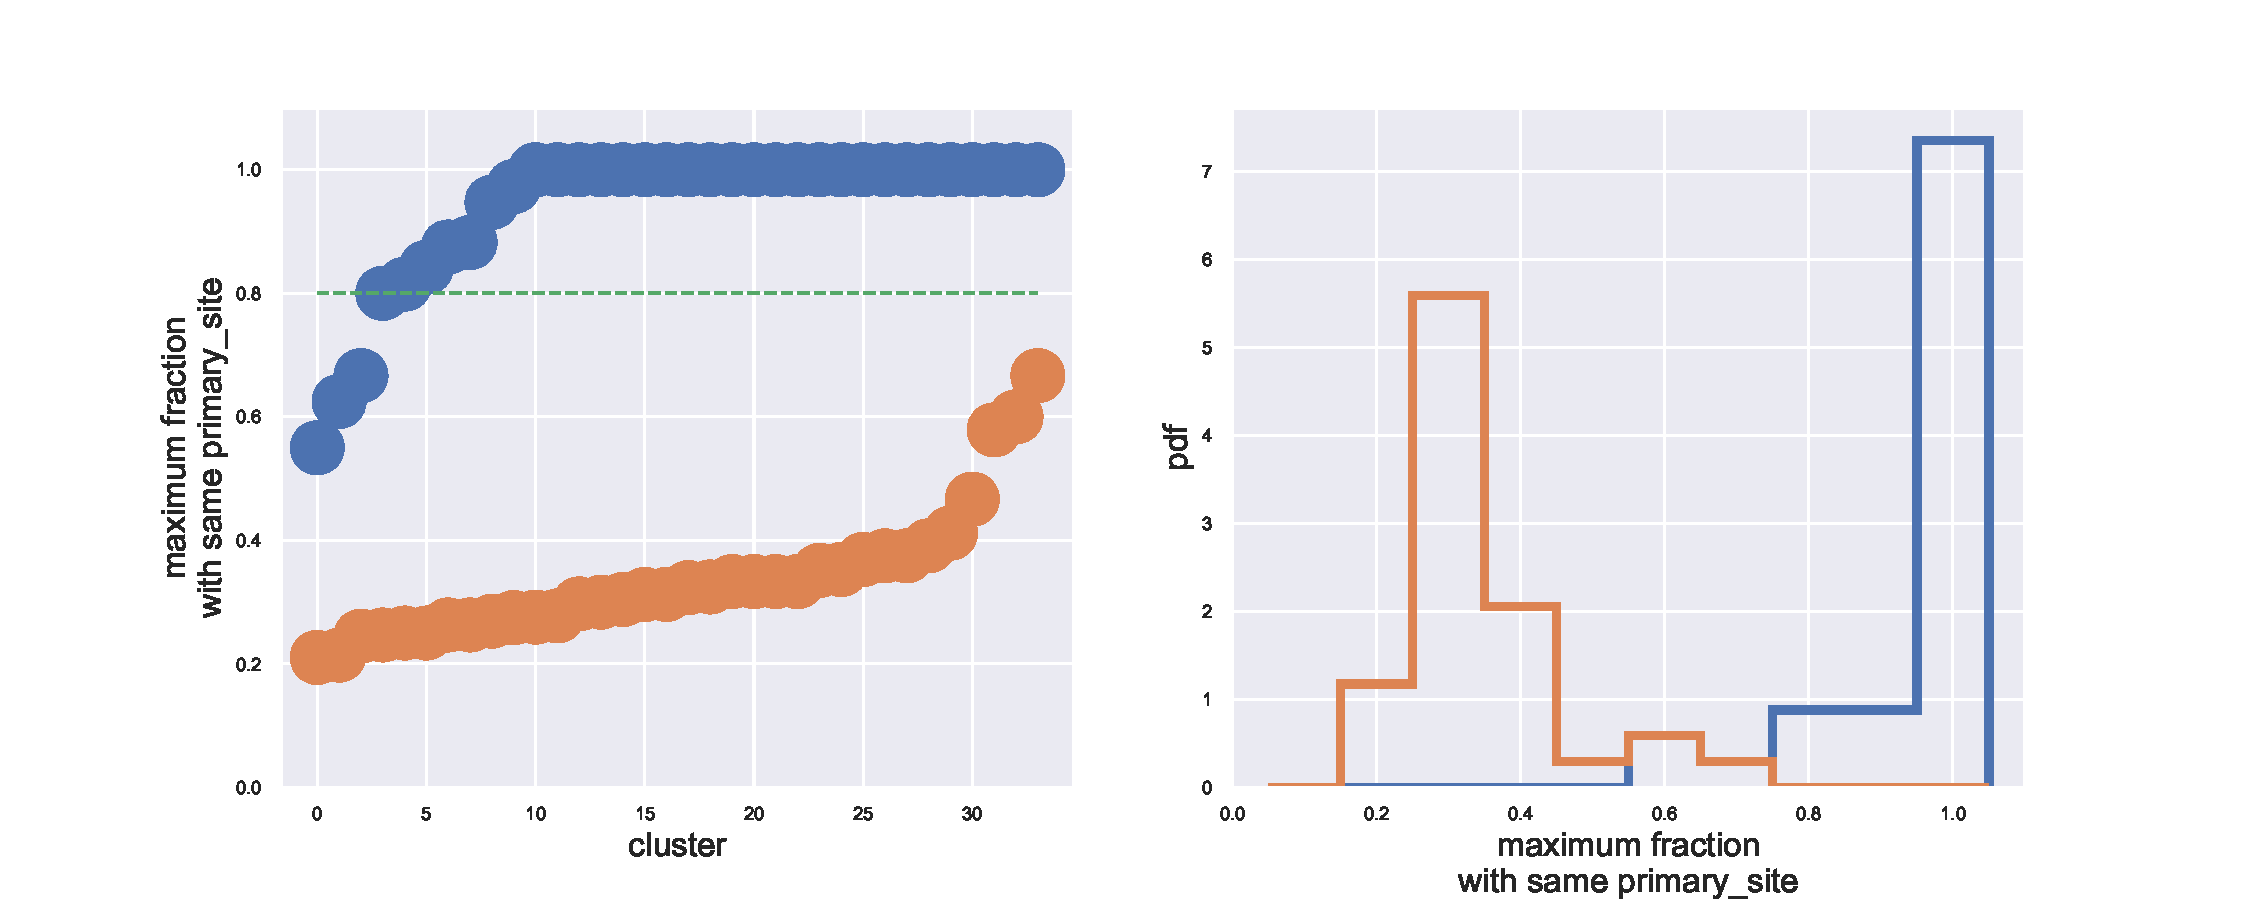
\includegraphics[width=0.9\linewidth]{pictures/topic/gtex/oversigma_10tissue/shuffledcluster_maximum_l2_primary_site.pdf}
    \caption{The fraction of cluster composed by the representative label versus cluster. On the right the distributions of this measure.}
    \label{fig:gtex/oversigma_10tissue/shuffledcluster_maximum_l2_primary_site}
\end{figure}
In figure~\ref{fig:topic/gtex/oversigma_10tissue/shuffledcluster_maximum*} the same analysis is done for every level of the hierarchy. It is interesting to notice that at deeper levels (upper left in the figure) the random reshuffling and the real labels have the same behaviour. This happens because, at this level, clusters are very small and so it is easier to pick up nodes with the same label (in the extreme case of a cluster with size 1 it is always full of the same label). This shows that the deepest level is not interesting: results are the same with random labels; moreover the reshuffling null model is good to show up eventual biases due to small cluster sizes.
\begin{figure}[htb!]
    \centering
    \begin{minipage}{0.45\textwidth}
    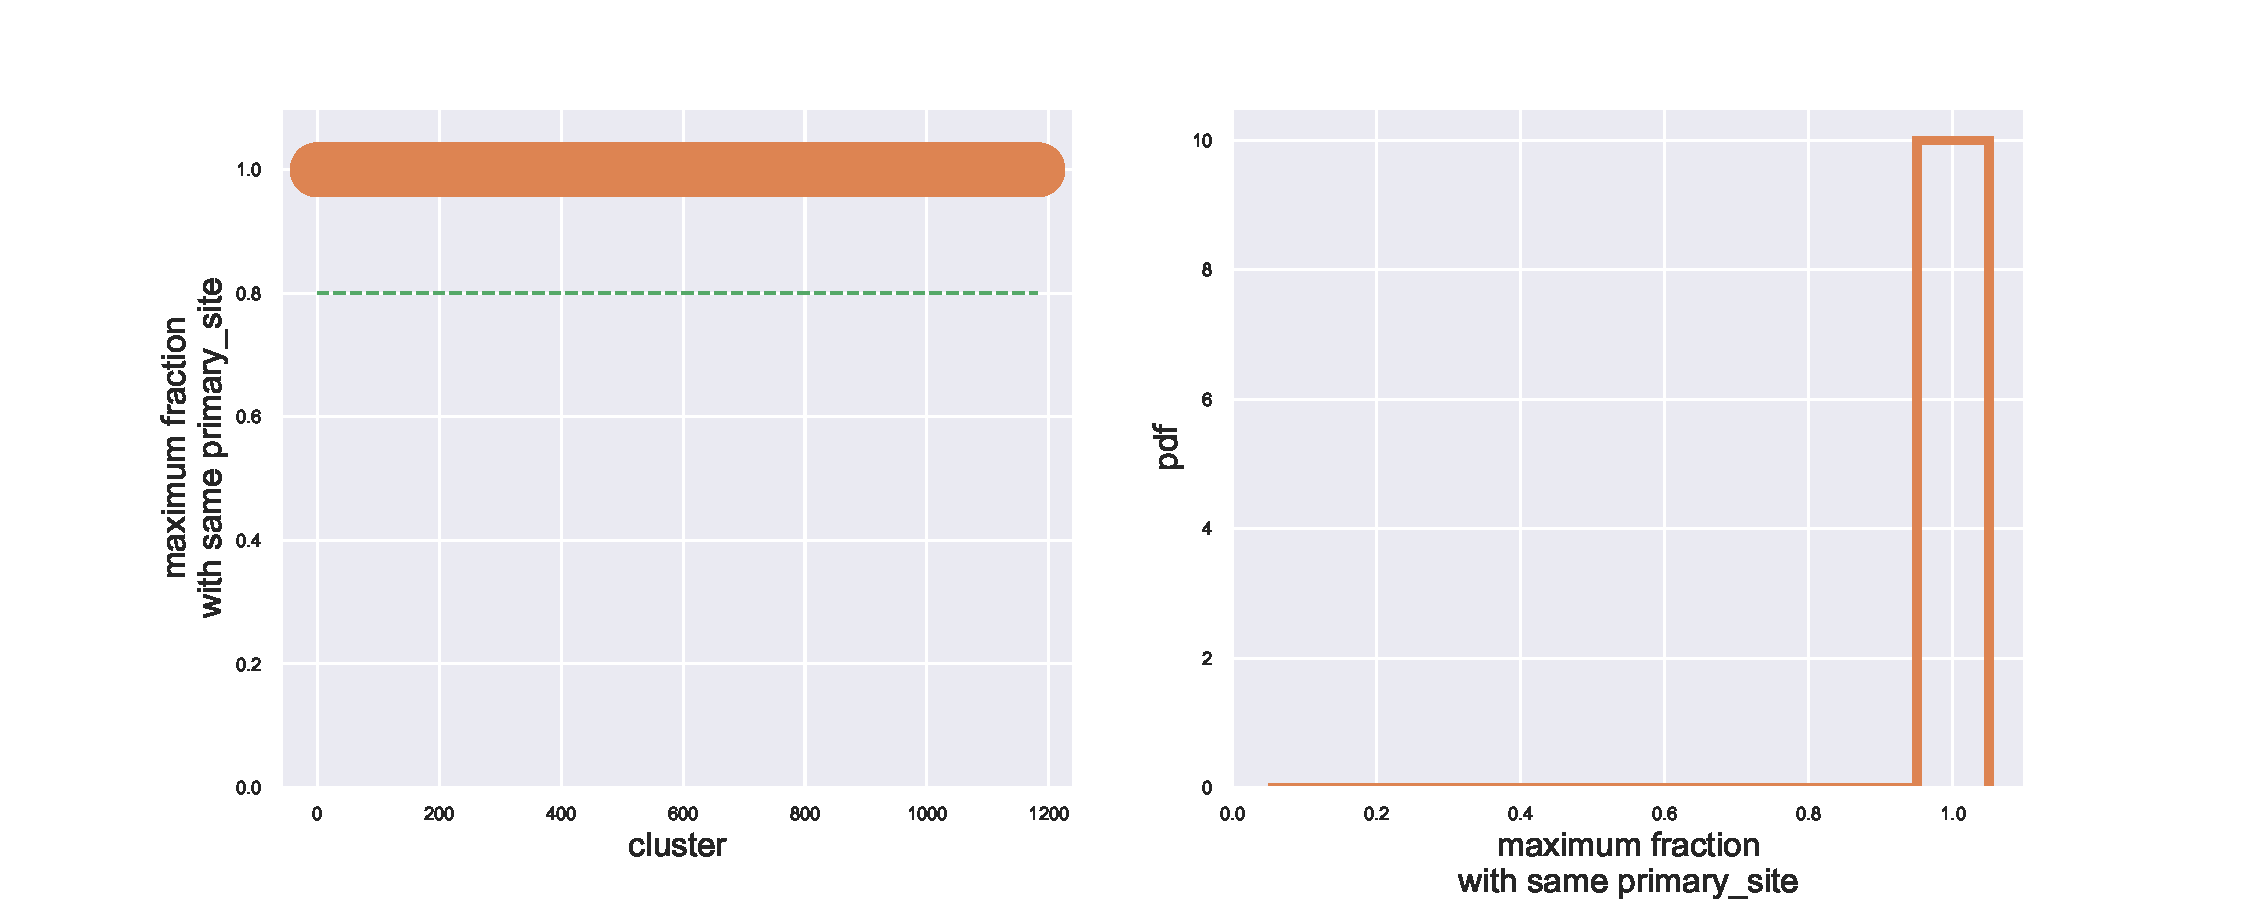
\includegraphics[width=0.9\linewidth]{pictures/topic/gtex/oversigma_10tissue/shuffledcluster_maximum_l0_primary_site.pdf}
    \end{minipage}
    \hspace{3mm}
    \begin{minipage}{0.45\textwidth}
    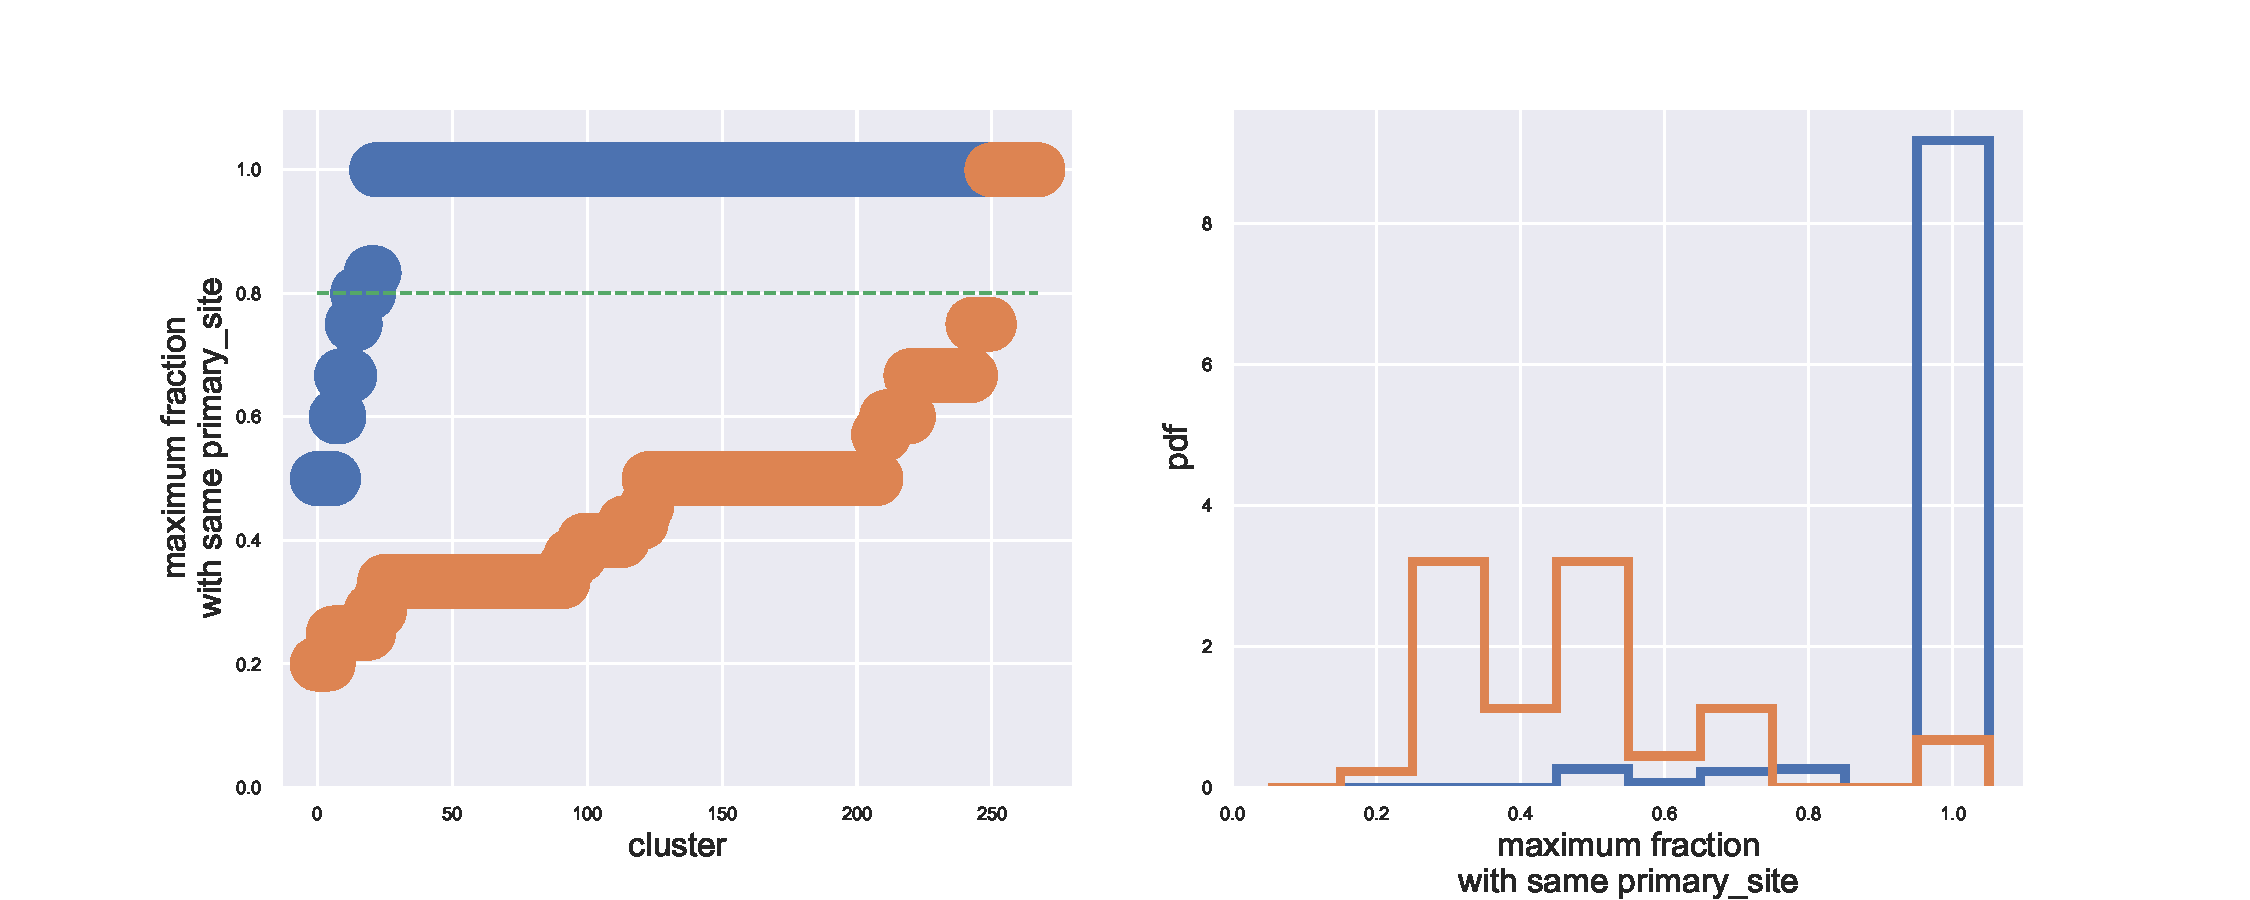
\includegraphics[width=0.9\linewidth]{pictures/topic/gtex/oversigma_10tissue/shuffledcluster_maximum_l1_primary_site.pdf}
    \end{minipage}
    \\
    \begin{minipage}{0.45\textwidth}
    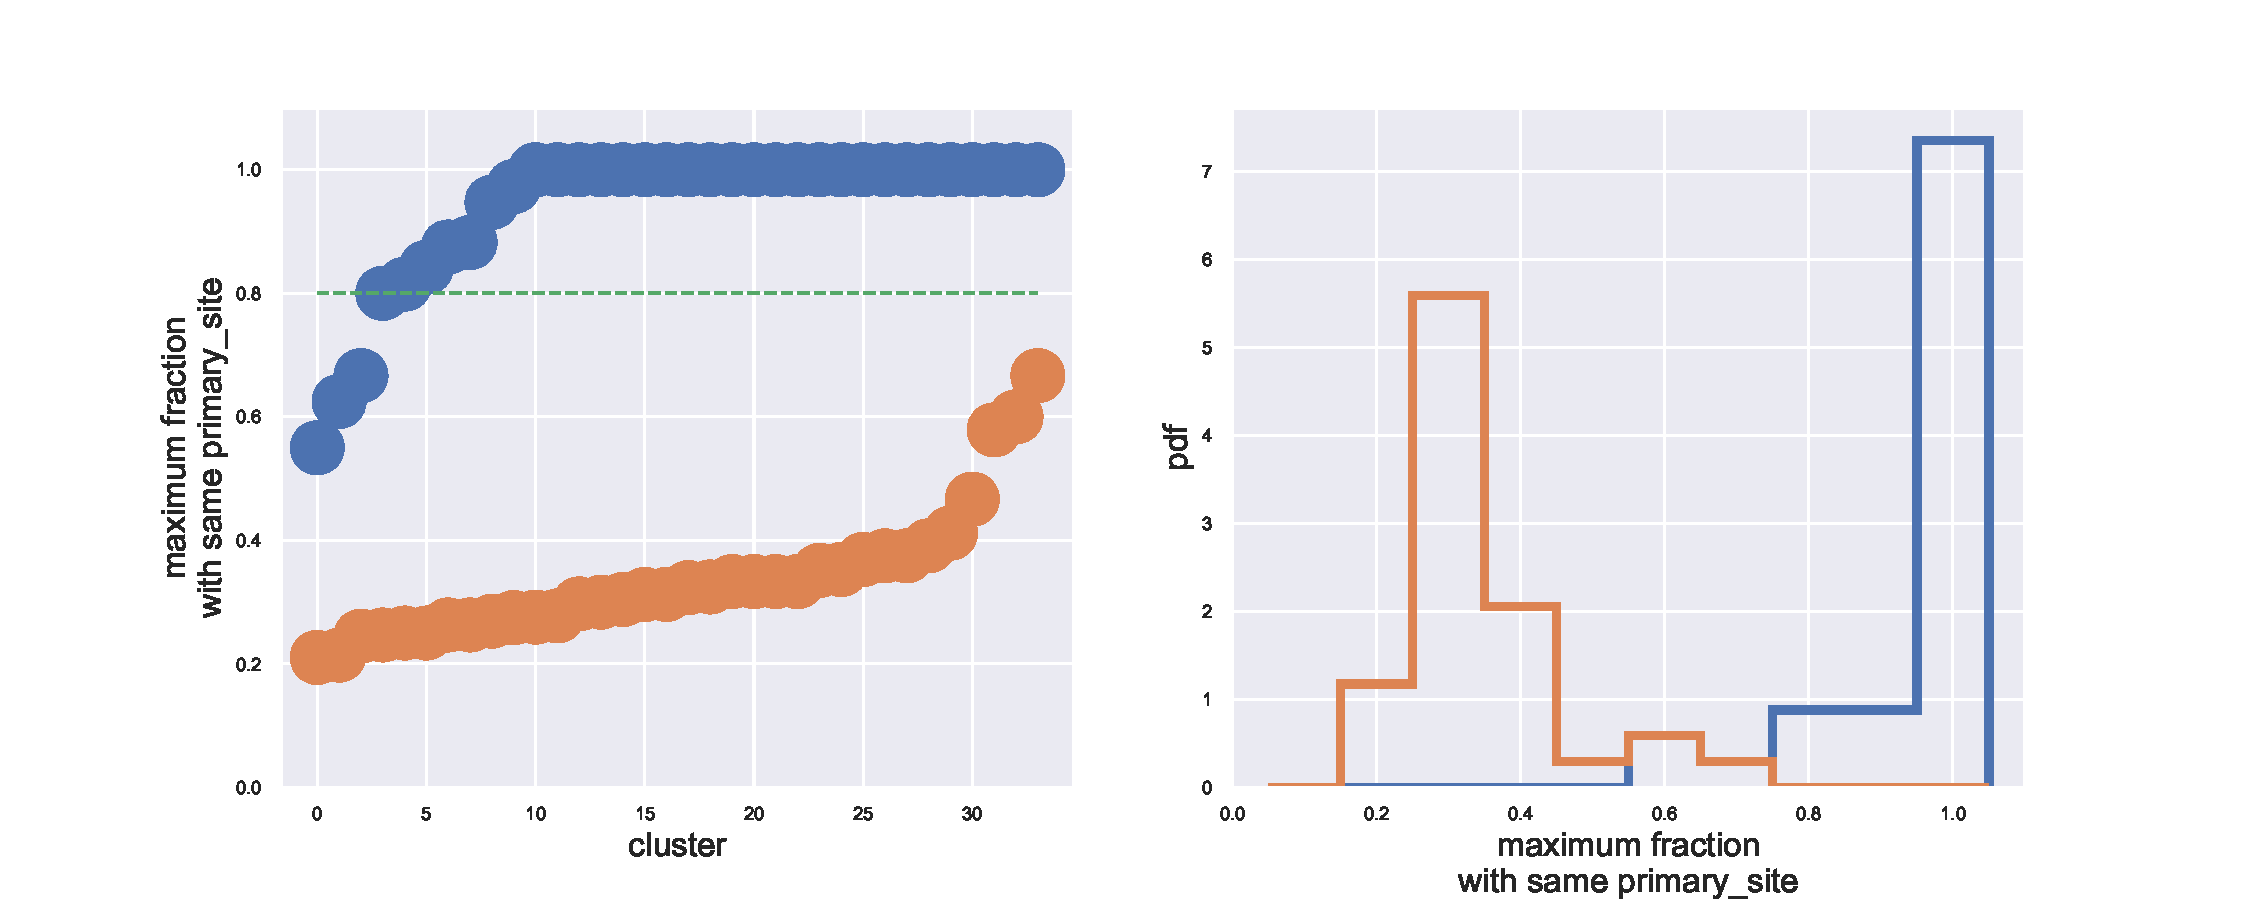
\includegraphics[width=0.9\linewidth]{pictures/topic/gtex/oversigma_10tissue/shuffledcluster_maximum_l2_primary_site.pdf}
    \end{minipage}
    \hspace{3mm}
    \begin{minipage}{0.45\textwidth}
    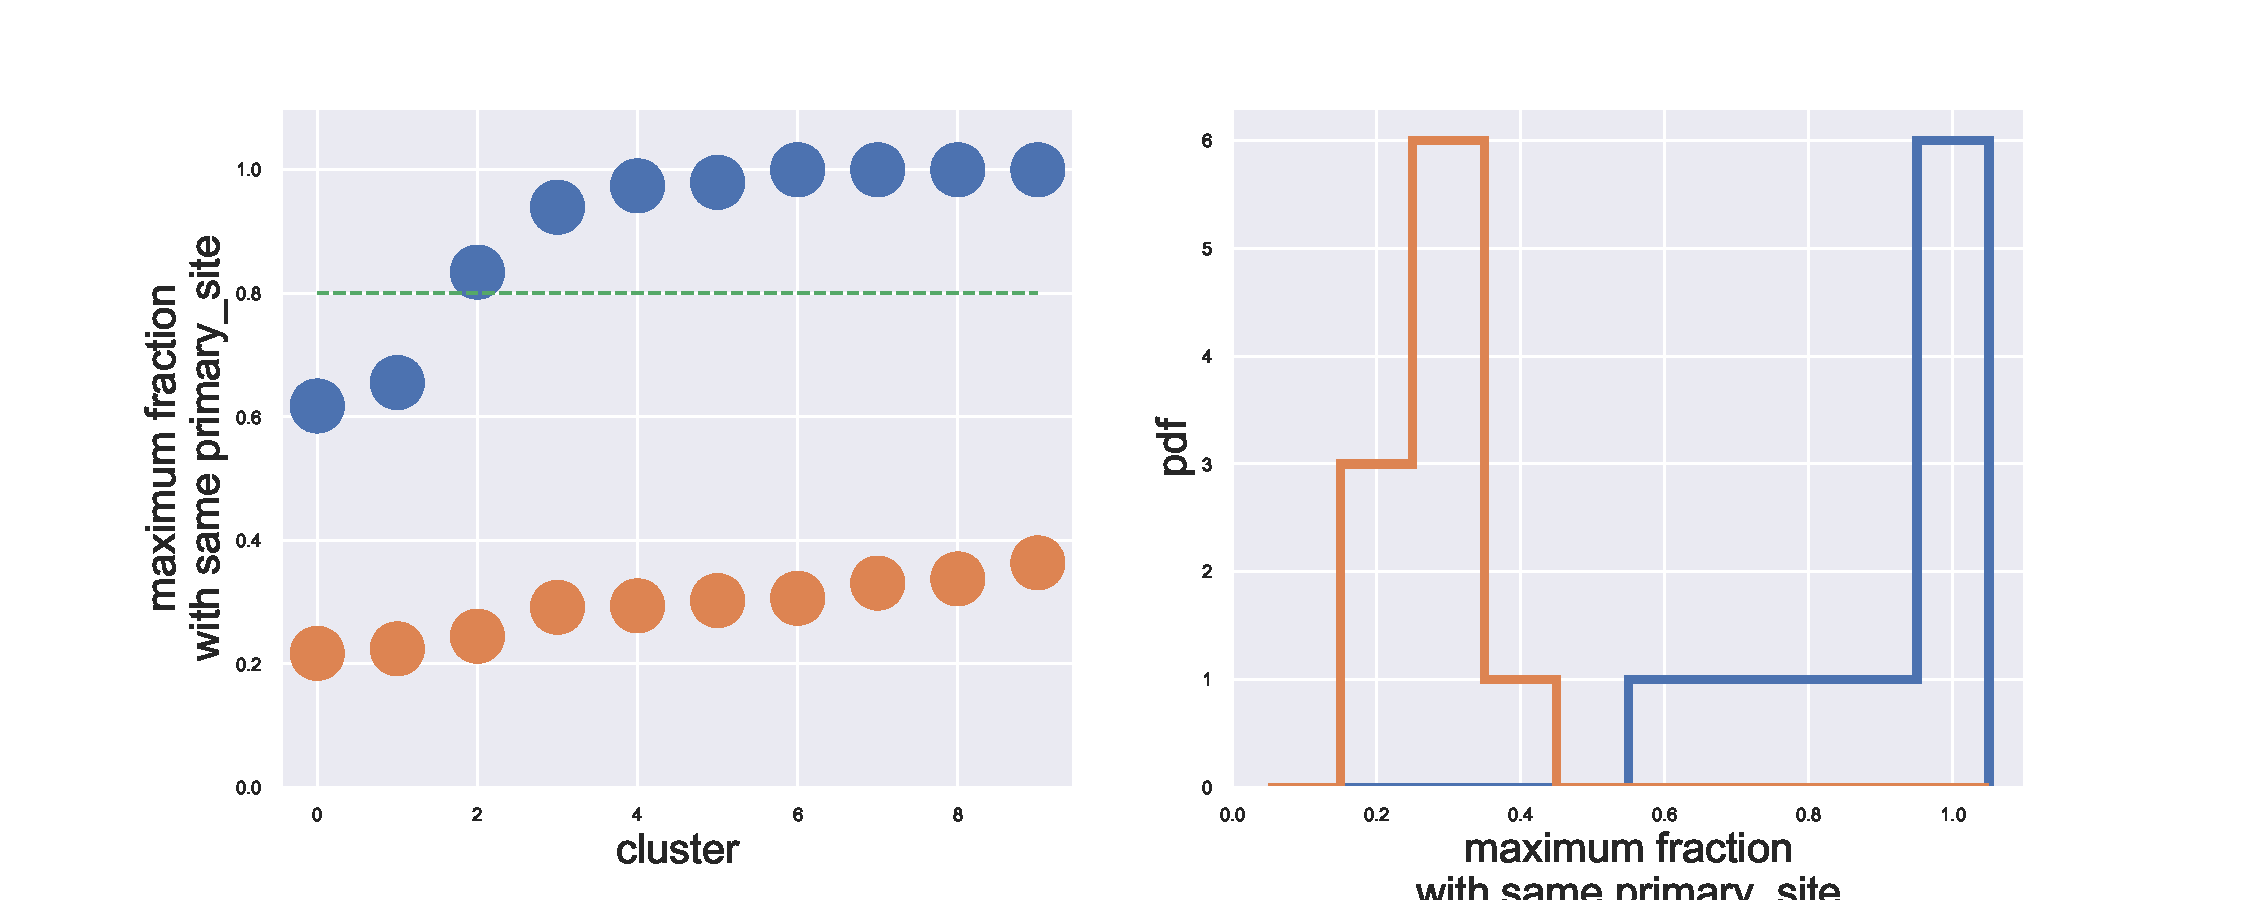
\includegraphics[width=0.9\linewidth]{pictures/topic/gtex/oversigma_10tissue/shuffledcluster_maximum_l3_primary_site.pdf}
    \end{minipage}
    \caption{The fraction of the most representative label in all clusters for different levels of the hierarchy. From upper left the deeper layer than downright the superficial one.}
    \label{fig:topic/gtex/oversigma_10tissue/shuffledcluster_maximum*}
\end{figure}
\FloatBarrier
A similar analysis can be made considering not just the number of the cluster but the cluster size, this is shown in figure~\ref{fig:topic/gtex/oversigma_10tissue/shuffledclusterhomosize_l3_primary_site}. It is interesting to notice that the shuffle null model and the real labels clusters are different, so there must be some kind of signal. Clearly the model is able to output even big clusters full of the same label (points upper right in figure~\ref{fig:topic/gtex/oversigma_10tissue/shuffledclusterhomosize_l3_primary_site}).
\begin{figure}[htb!]
	\centering
	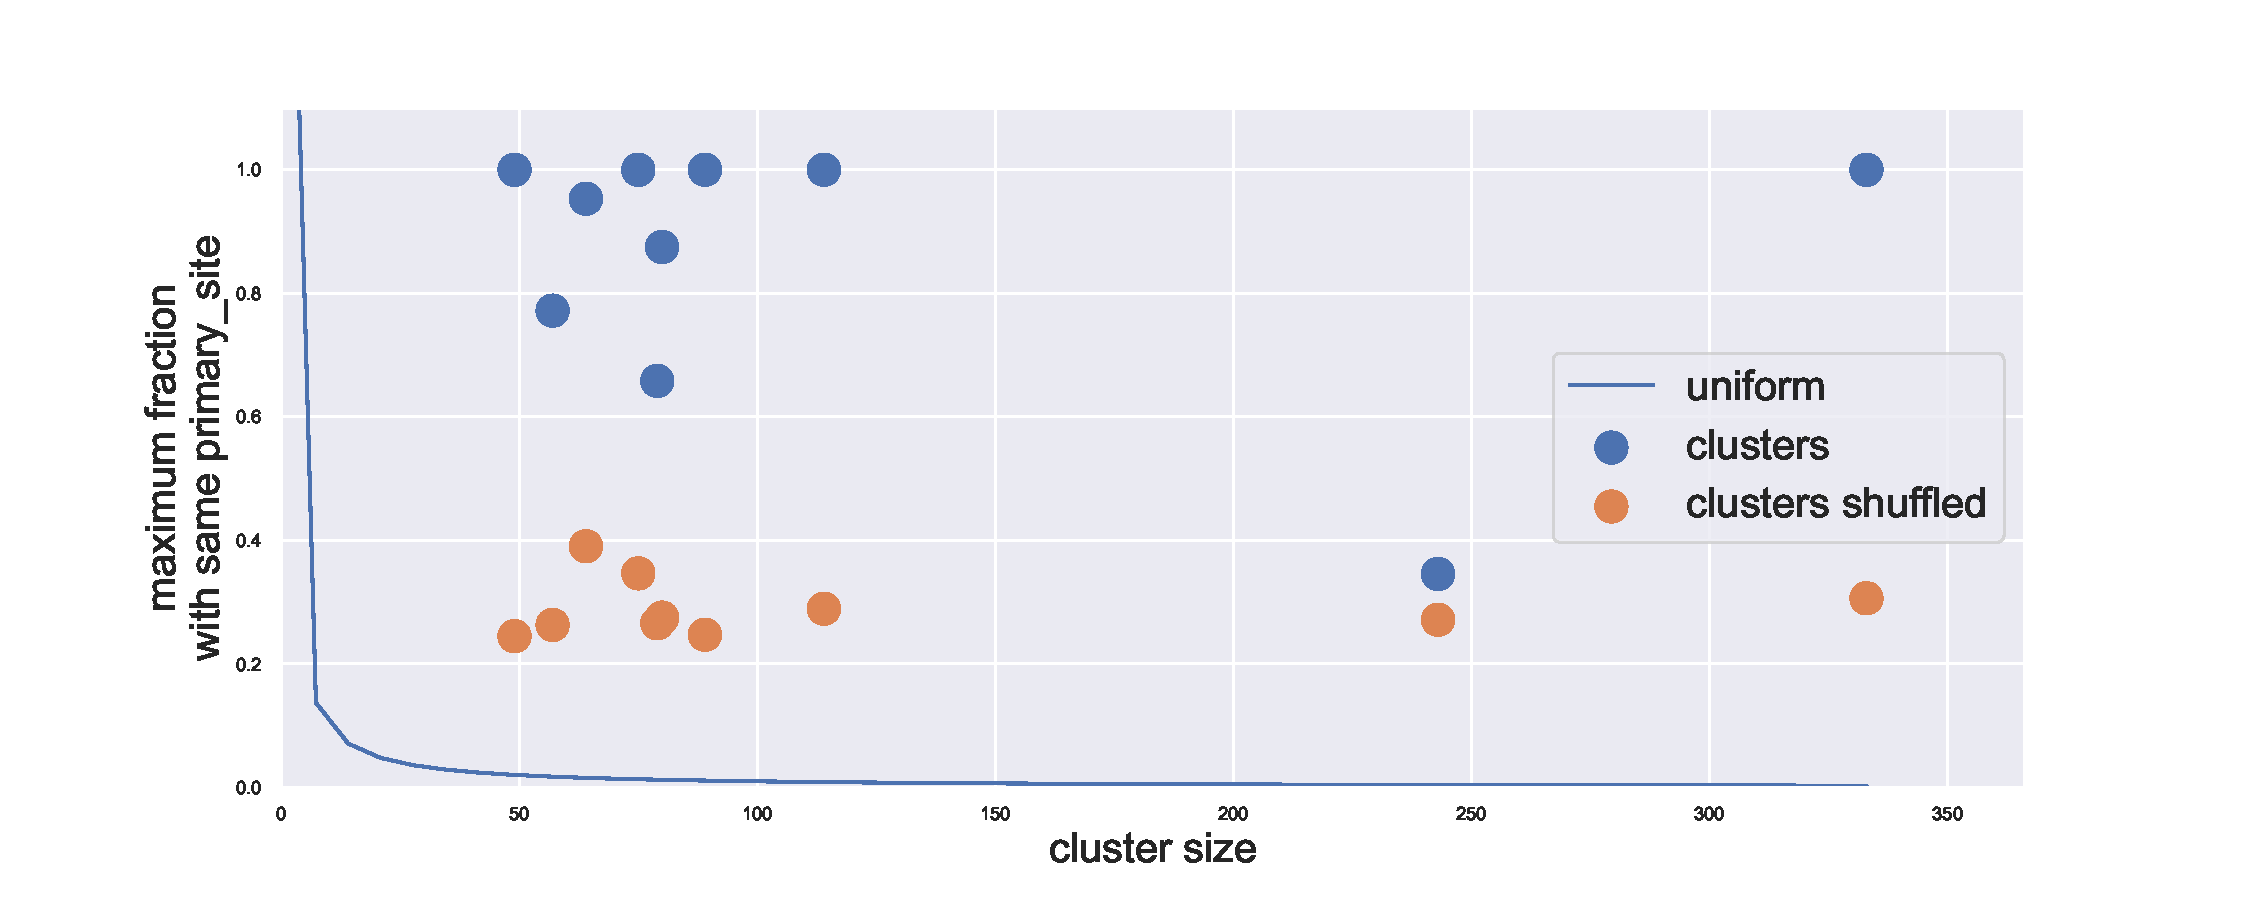
\includegraphics[width=0.9\linewidth]{pictures/topic/gtex/oversigma_10tissue/shuffledclusterhomosize_l3_primary_site.pdf}
	\caption{The fraction of the most representative label versus cluster size.}
	\label{fig:topic/gtex/oversigma_10tissue/shuffledclusterhomosize_l3_primary_site}
\end{figure}
In figure~\ref{fig:topic/gtex/oversigma_10tissue/shuffledclusterhomosize_l*} the same analysis for all the levels of the hierarchy. It is interesting to see how going up in the hierarchy the two signals become different, as shown before the deeper layer (upper left in the image) is not different from null model and so it is not interesting.
\begin{figure}[htb!]
	\centering
	\begin{minipage}{0.45\textwidth}
		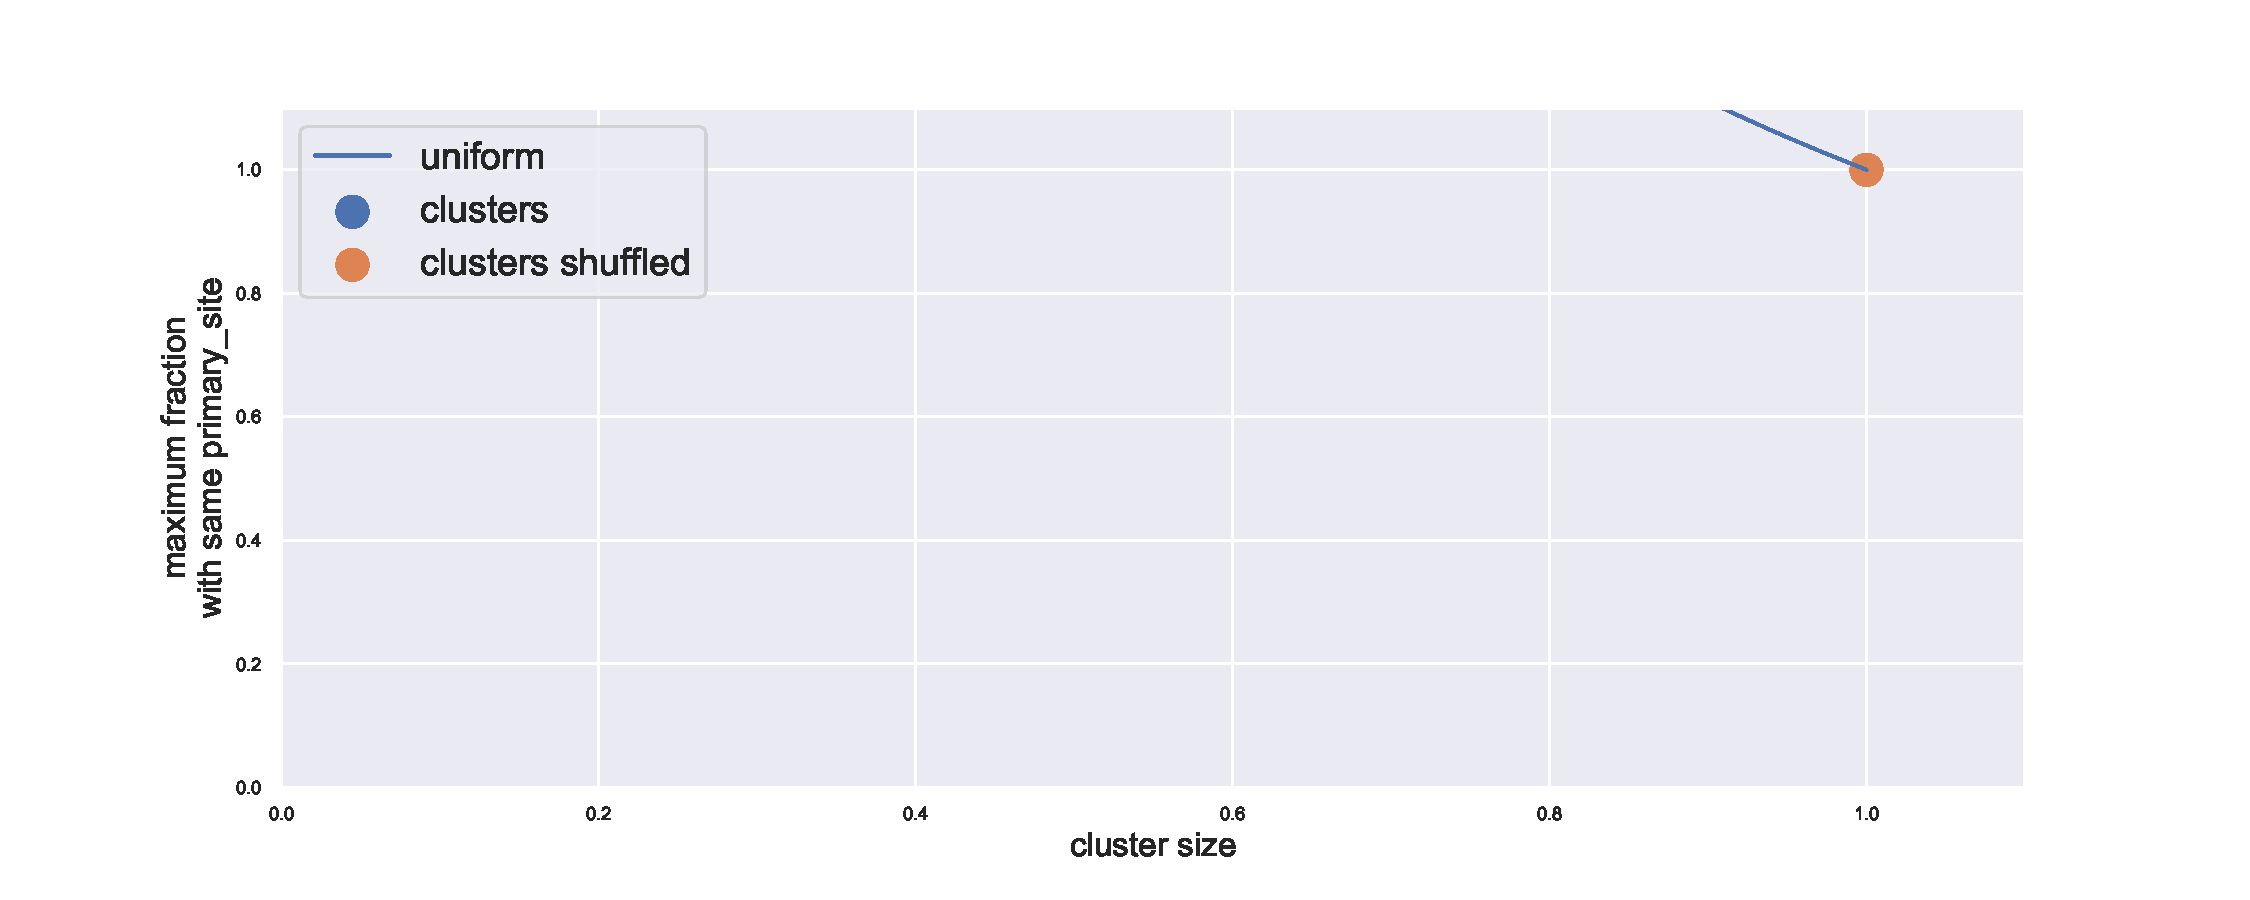
\includegraphics[width=0.9\linewidth]{pictures/topic/gtex/oversigma_10tissue/shuffledclusterhomosize_l0_primary_site.pdf}
	\end{minipage}
	\hspace{3mm}
	\begin{minipage}{0.45\textwidth}
		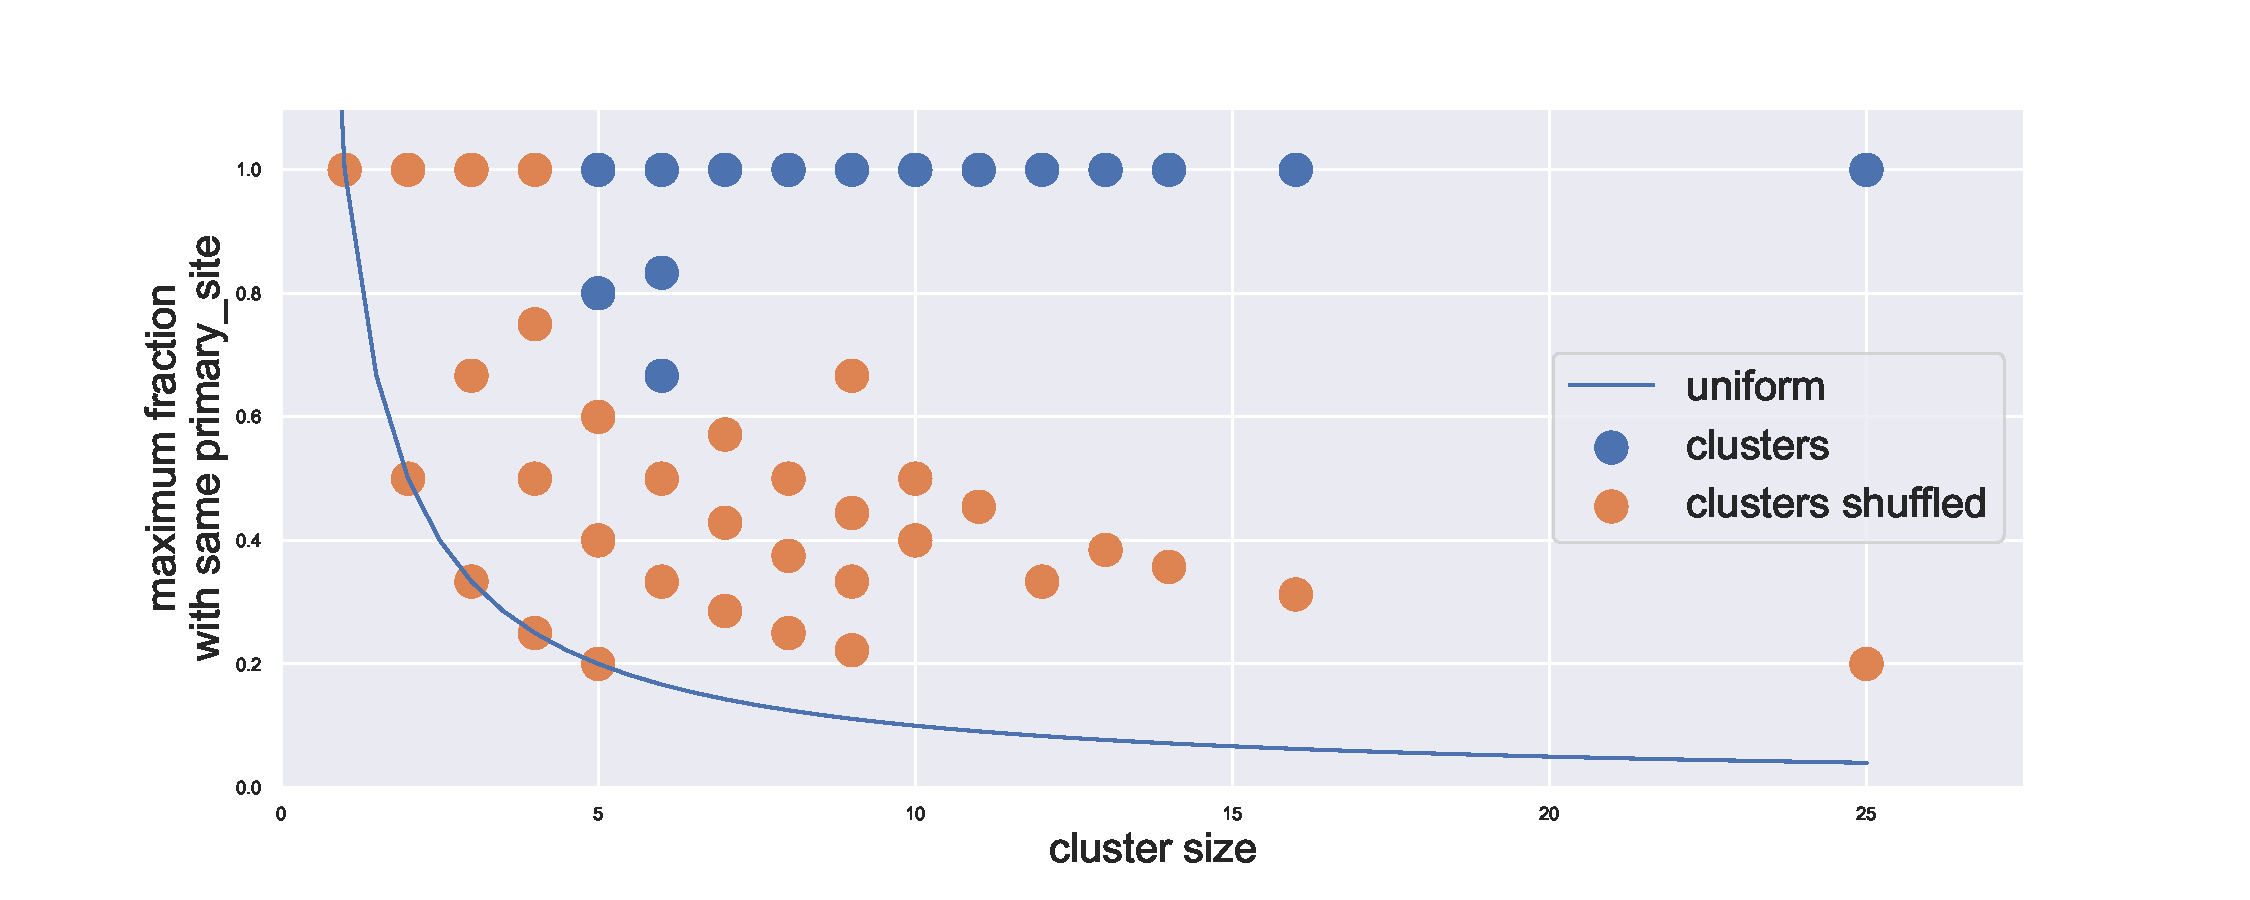
\includegraphics[width=0.9\linewidth]{pictures/topic/gtex/oversigma_10tissue/shuffledclusterhomosize_l1_primary_site.pdf}
	\end{minipage}
	\\
	\begin{minipage}{0.45\textwidth}
		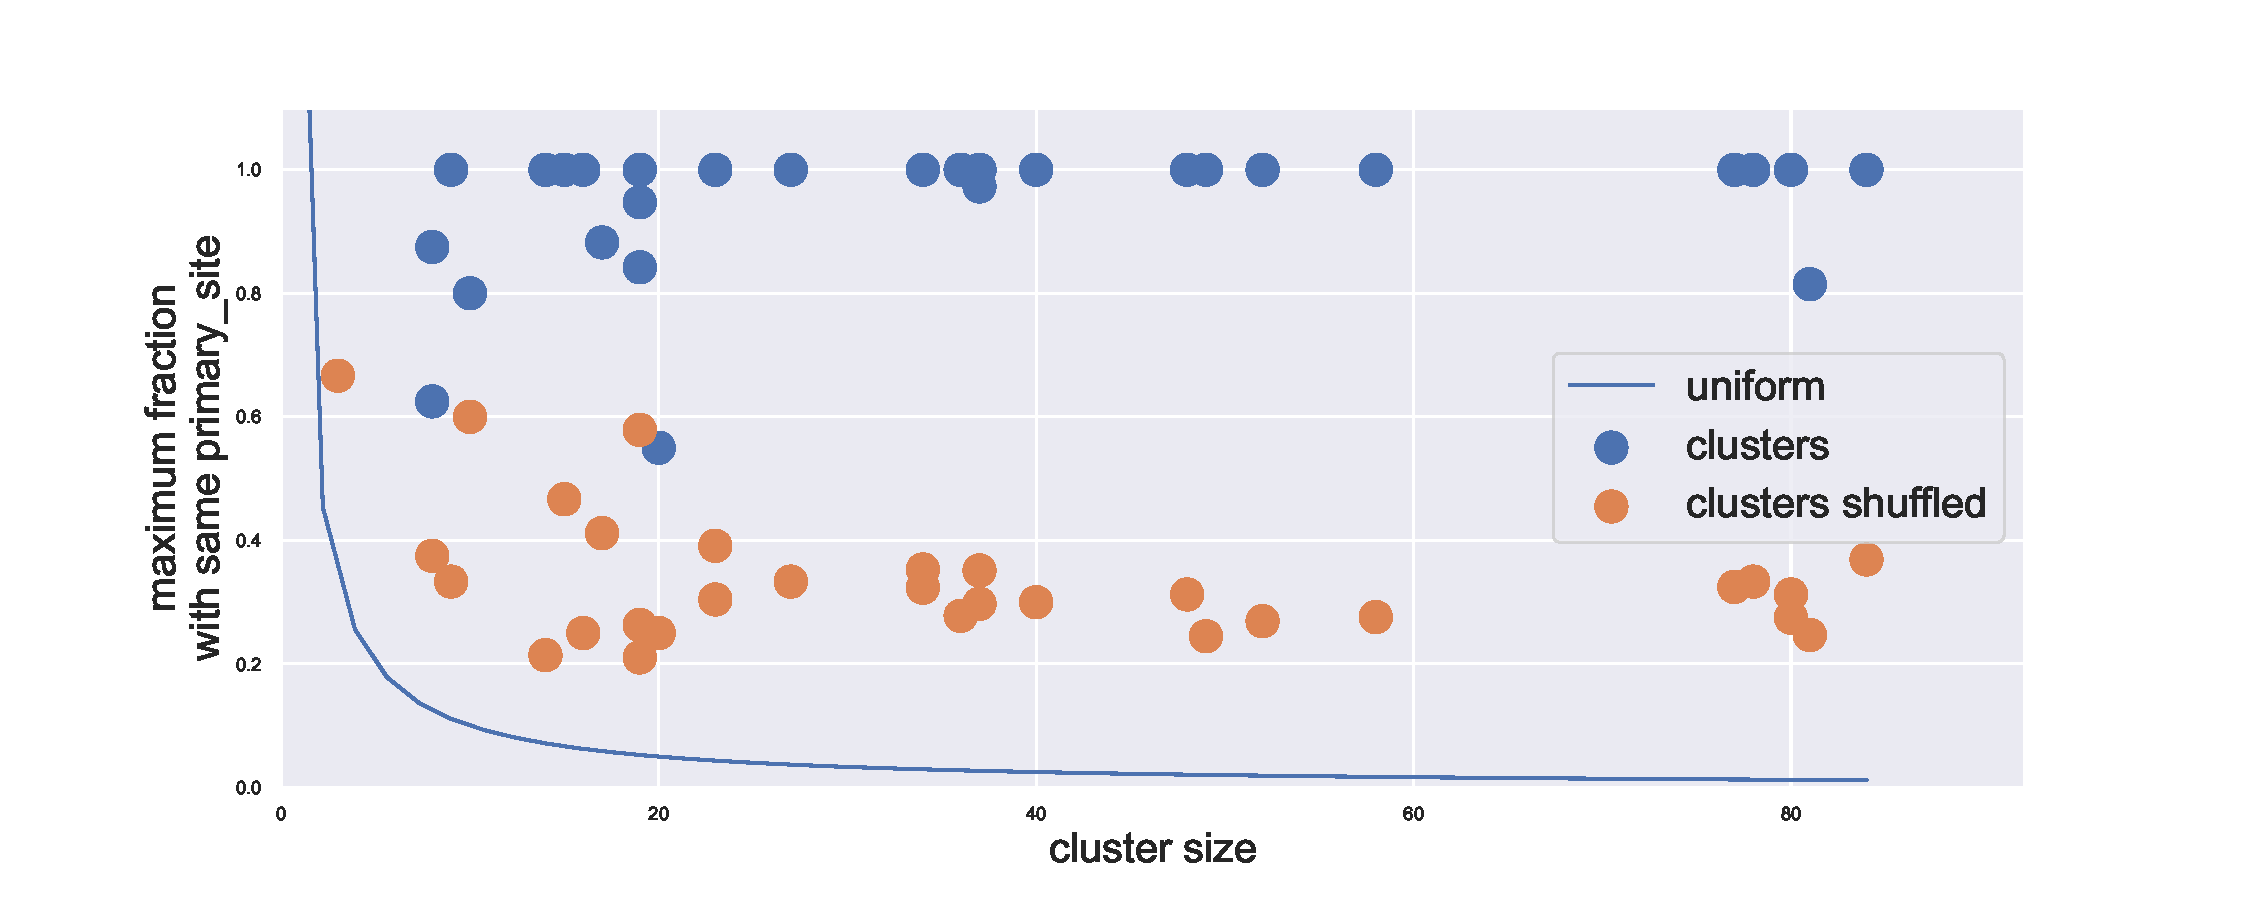
\includegraphics[width=0.9\linewidth]{pictures/topic/gtex/oversigma_10tissue/shuffledclusterhomosize_l2_primary_site.pdf}
	\end{minipage}
	\hspace{3mm}
	\begin{minipage}{0.45\textwidth}
		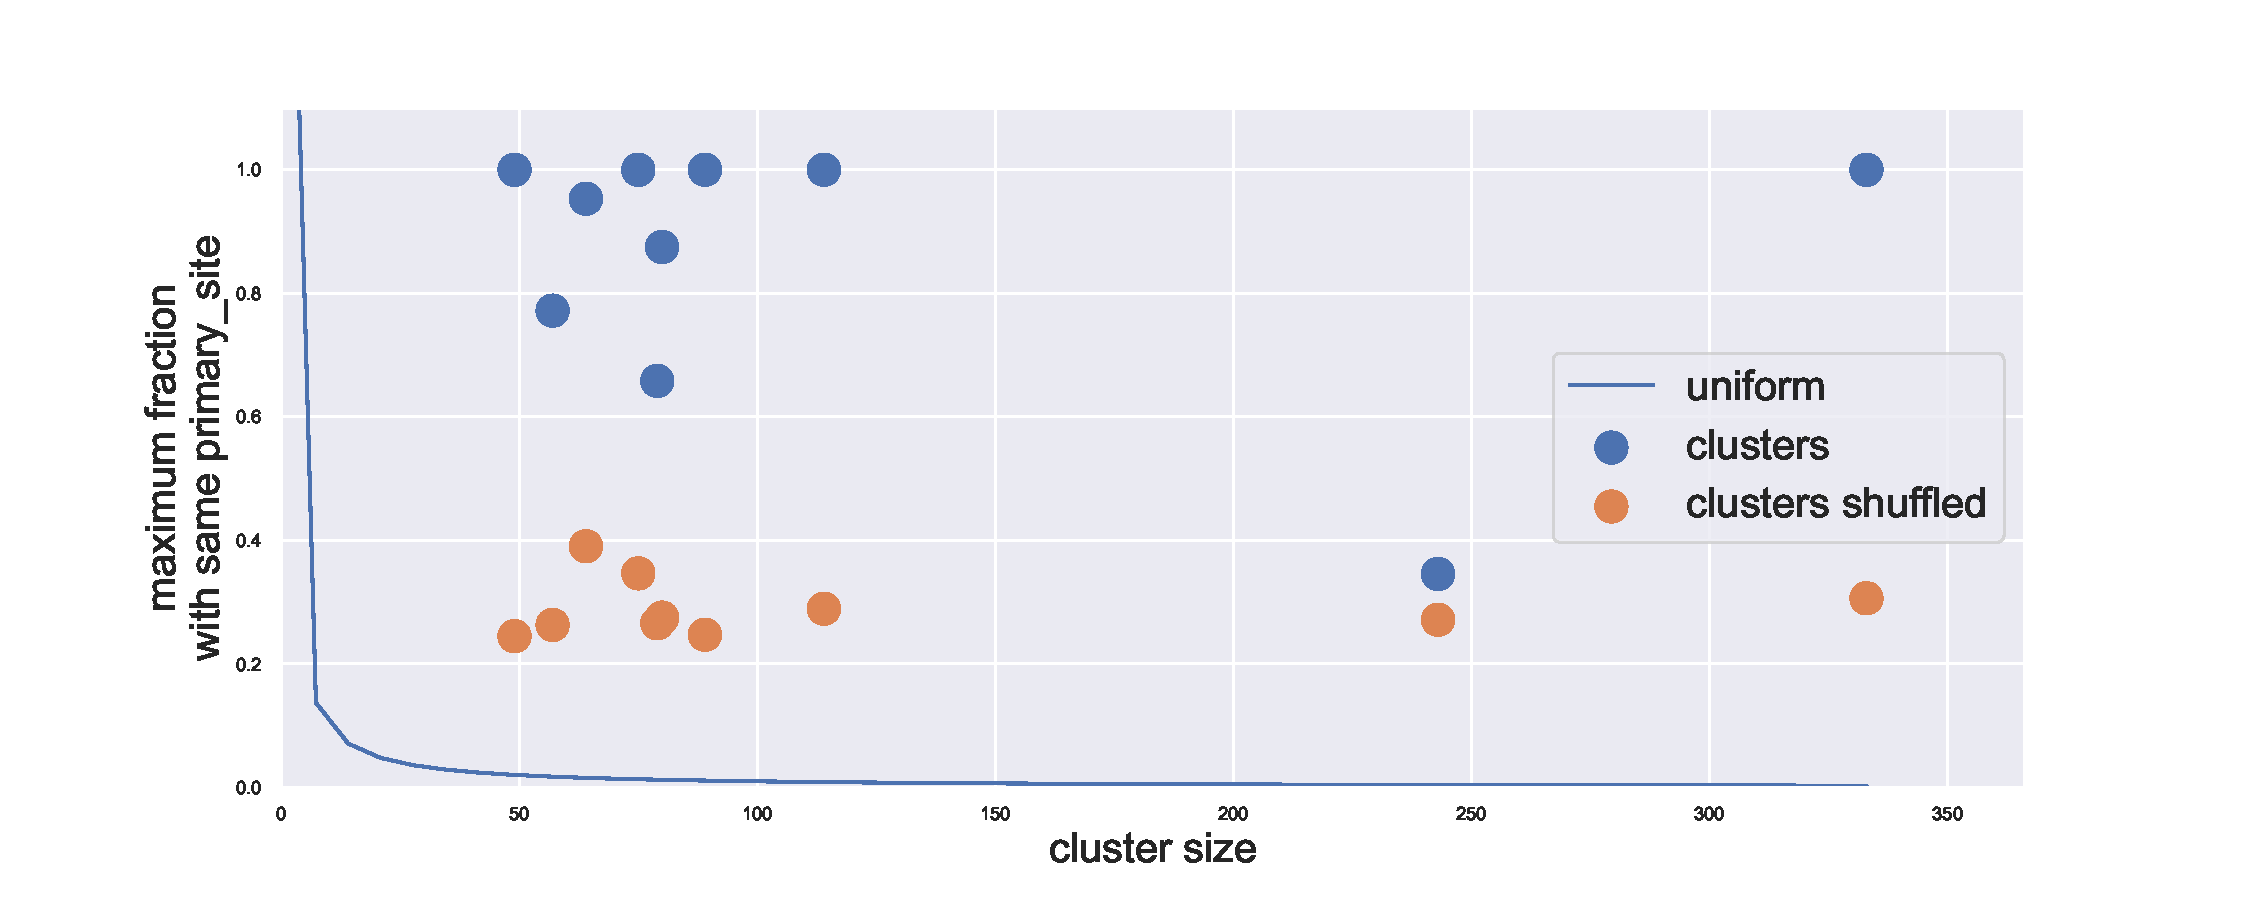
\includegraphics[width=0.9\linewidth]{pictures/topic/gtex/oversigma_10tissue/shuffledclusterhomosize_l3_primary_site.pdf}
	\end{minipage}
	\caption{The fraction of the most representative label versus cluster size across the hierarchy. From upper left the deeper layer than downright the superficial one.}
	\label{fig:topic/gtex/oversigma_10tissue/shuffledclusterhomosize_l*}
\end{figure}
\FloatBarrier
At this point to investigate deeper the structure of the clusters, it can be interesting to study how many labels are present in each cluster. The fraction of the most represented label defined above carries no information of what happens to the remaining labels. For example, if one cluster is composed of $80\%$ by label \textbf{A} and $20\%$ by label \textbf{B} and another cluster is composed $80\%$ by label \textbf{A}, $10\%$ by label \textbf{B} and $10\%$ by label \textbf{C} they have both a fraction of maximum representative label $80\%$ but the second in this example is more heterogeneous. Counting the number of different labels in each cluster can reveal this kind of effects. In figure~\ref{fig:topic/gtex/oversigma_10tissue/shuffledcluster_shuffle_label_size_l3_primary_site} it is represented the number of different labels versus cluster size. It is evident that the reshuffling case is quite different from the real one, almost every cluster in the null model has got every label. It is interesting to notice that the model outputs even big cluster with one label.
\begin{figure}[htb!]
    \centering
    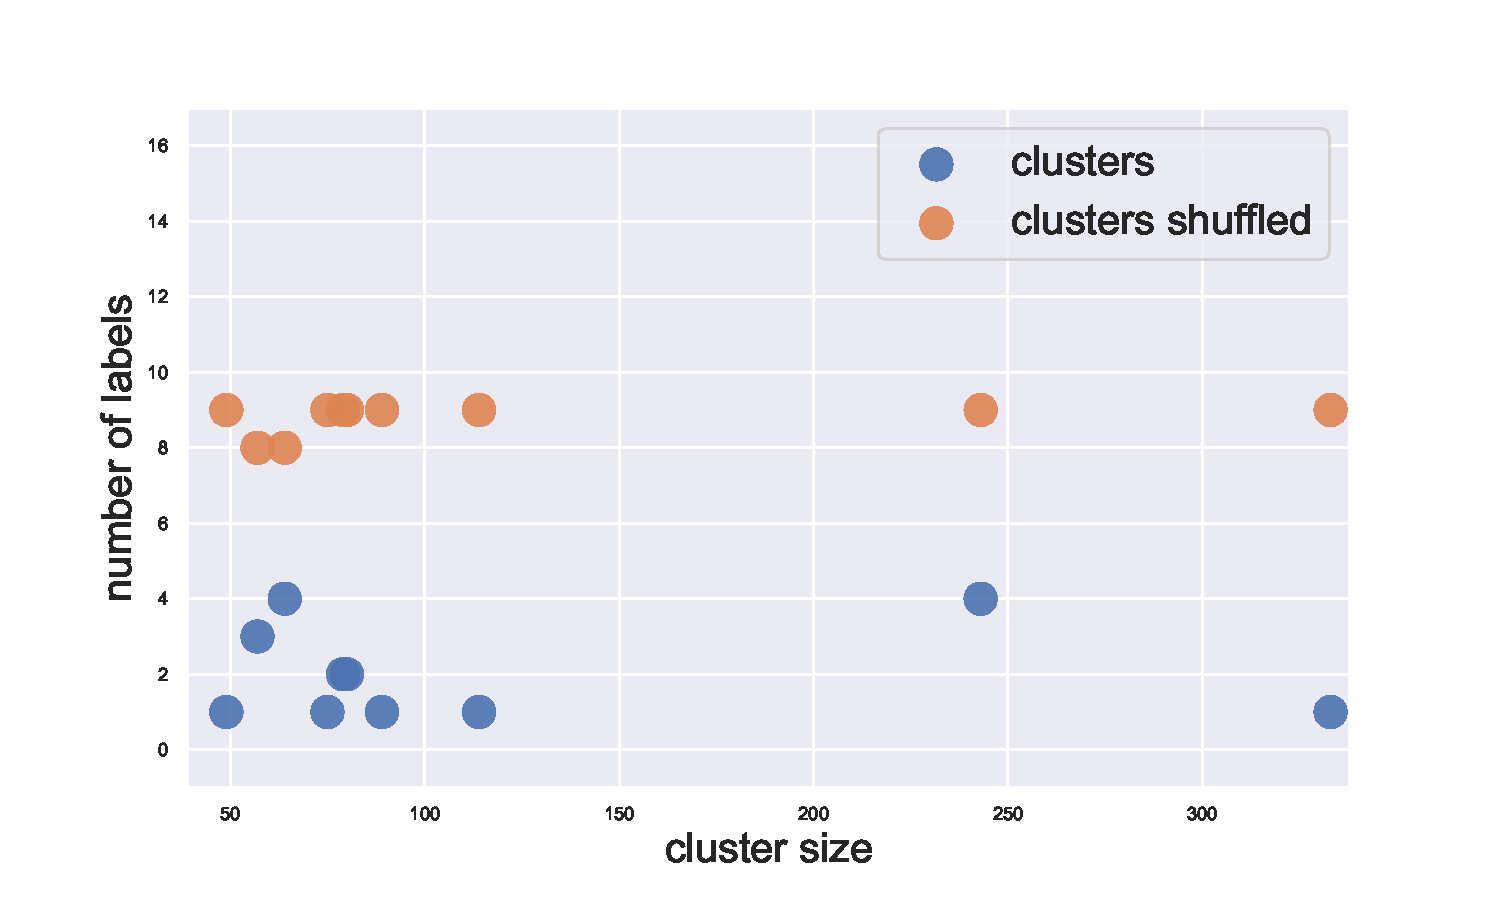
\includegraphics[width=0.9\linewidth]{pictures/topic/gtex/oversigma_10tissue/shuffledcluster_shuffle_label_size_l3_primary_site.pdf}
    \caption{The number of different labels in each cluster versus cluster size.}
    \label{fig:topic/gtex/oversigma_10tissue/shuffledcluster_shuffle_label_size_l3_primary_site}
\end{figure}
In figure~\ref{fig:topic/gtex/oversigma_10tissue/shuffledcluster_shuffle_label_size_lall} the same analysis for all the layer of the hierarchy. Even here the deeper level does not differ from the null model. Nevertheless, in layers with higher V-measure score, there is a strong signal that the reshuffling model is quite different from the model's output.
\begin{figure}[htb!]
    \centering
    \begin{minipage}{0.45\textwidth}
    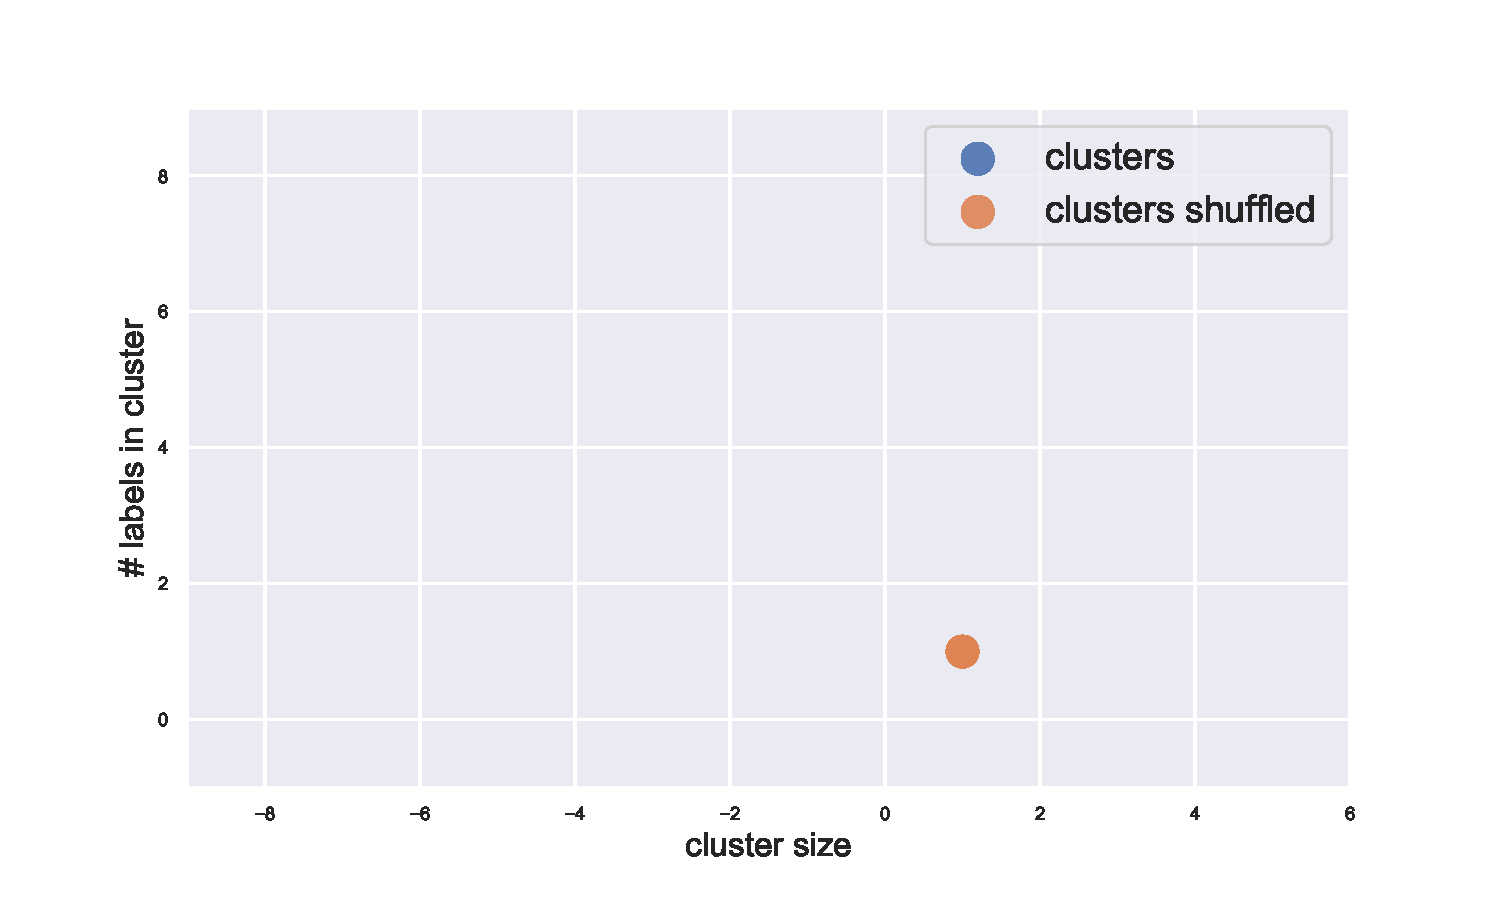
\includegraphics[width=0.9\linewidth]{pictures/topic/gtex/oversigma_10tissue/shuffledcluster_shuffle_label_size_l0_primary_site.pdf}
    \end{minipage}
    \hspace{3mm}
    \begin{minipage}{0.45\textwidth}
    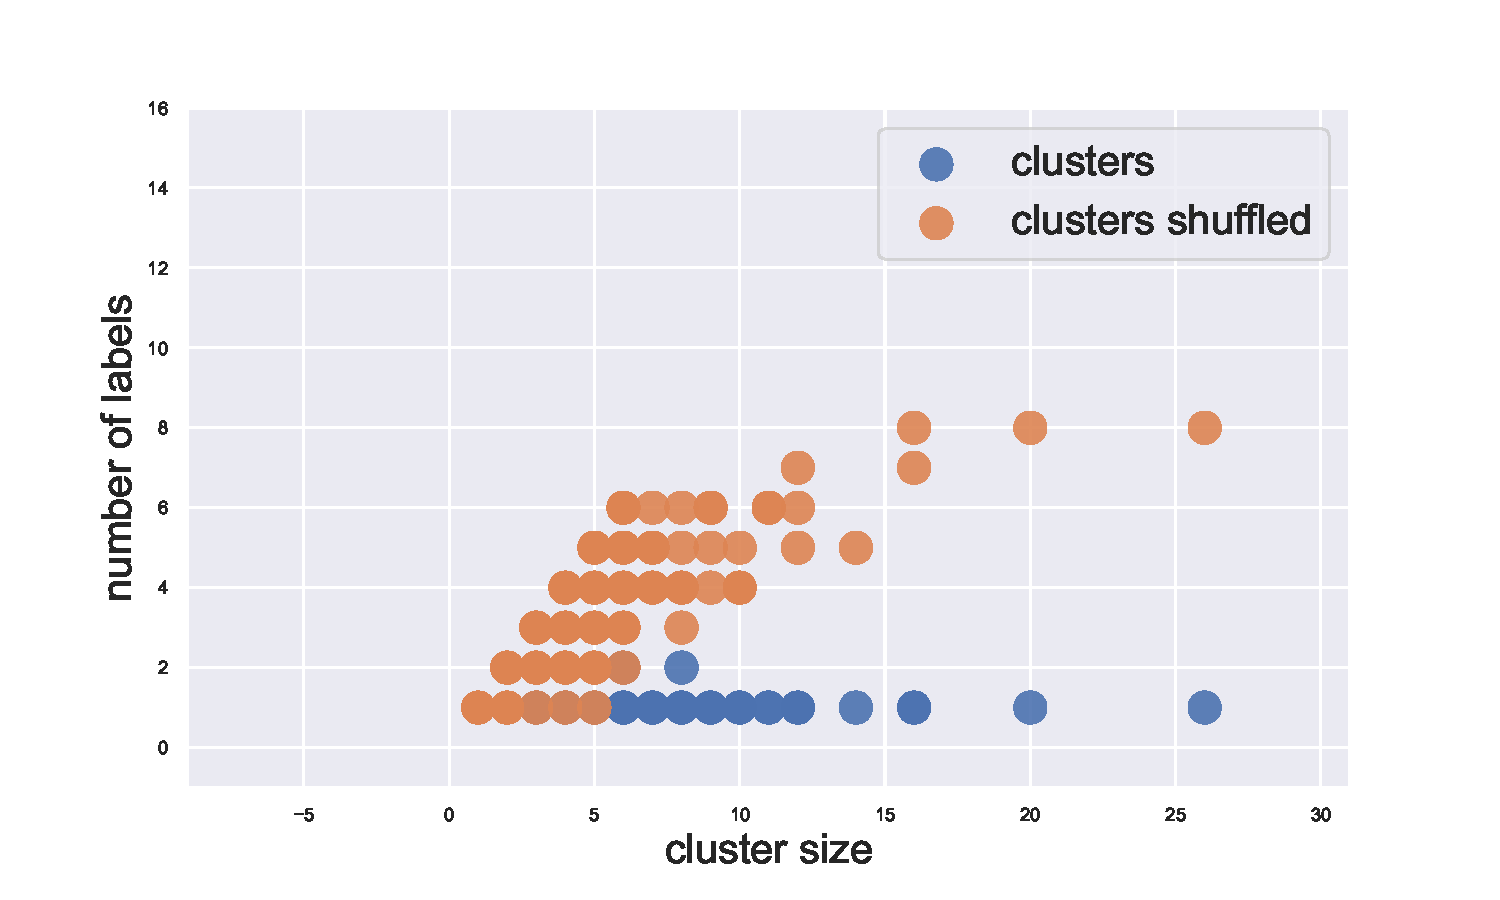
\includegraphics[width=0.9\linewidth]{pictures/topic/gtex/oversigma_10tissue/shuffledcluster_shuffle_label_size_l1_primary_site.pdf}
    \end{minipage}
    \\
    \begin{minipage}{0.45\textwidth}
    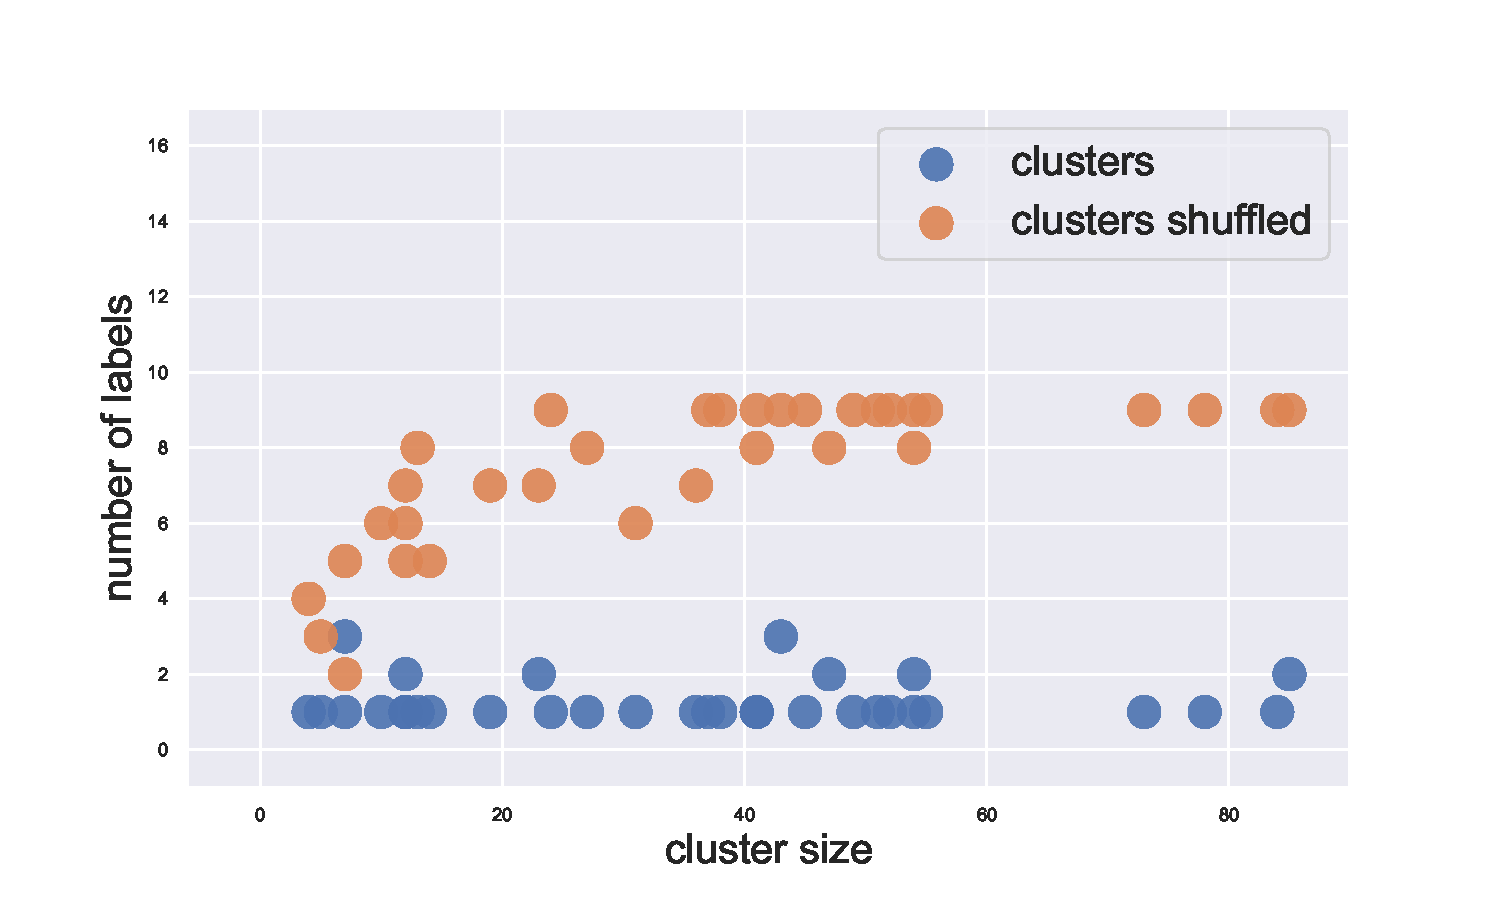
\includegraphics[width=0.9\linewidth]{pictures/topic/gtex/oversigma_10tissue/shuffledcluster_shuffle_label_size_l2_primary_site.pdf}
    \end{minipage}
    \hspace{3mm}
    \begin{minipage}{0.45\textwidth}
    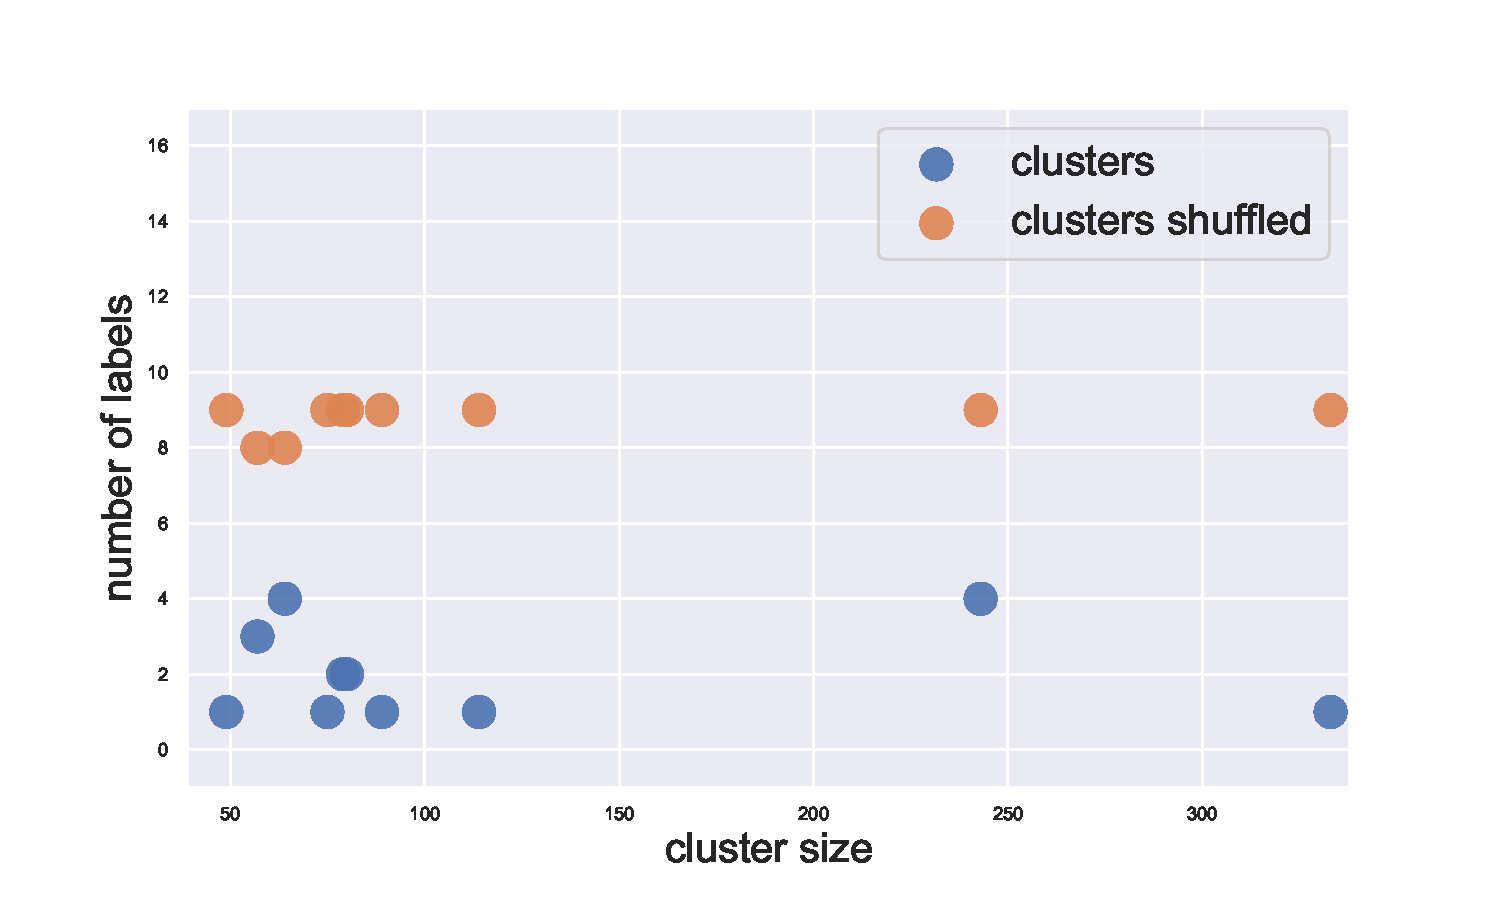
\includegraphics[width=0.9\linewidth]{pictures/topic/gtex/oversigma_10tissue/shuffledcluster_shuffle_label_size_l3_primary_site.pdf}
    \end{minipage}
\caption{The number of different labels in each cluster versus cluster size. From upper left the deeper layer than downright the superficial one.}
\label{fig:topic/gtex/oversigma_10tissue/shuffledcluster_shuffle_label_size_lall}
\end{figure}
\FloatBarrier
Having constructed the null model it is possible to estimate the V-measure score also for the null model. The results are reported in figure~\ref{fig:topic/gtex/oversigma_10tissue/metric_scores_shuffle}. 
Moreover, remembering the V-measure or normalized mutual information defined in~\ref{eq:mutualinformation} it is possible to estimate a mixed score which considers the homogeneity of the primary site and the completeness of the secondary site, doing so the score goes up if going deeper in the hierarchy the model makes more cluster with the same tissue but separates sub-tissues. It is not a big deal if one loses completeness regarding tissues (the model separates one big cluster full of the same label into two small ones) but gain information at the next resolution. This becomes clear if one looks at the big \textit{blood} cluster that in the next level of the hierarchy is separated into two clusters of \textit{blood}, one of \textit{whole blood} and one of \textit{lymphocytes}. The result is that this mixed score is the highest one.
\begin{figure}[htb!]
    \centering
    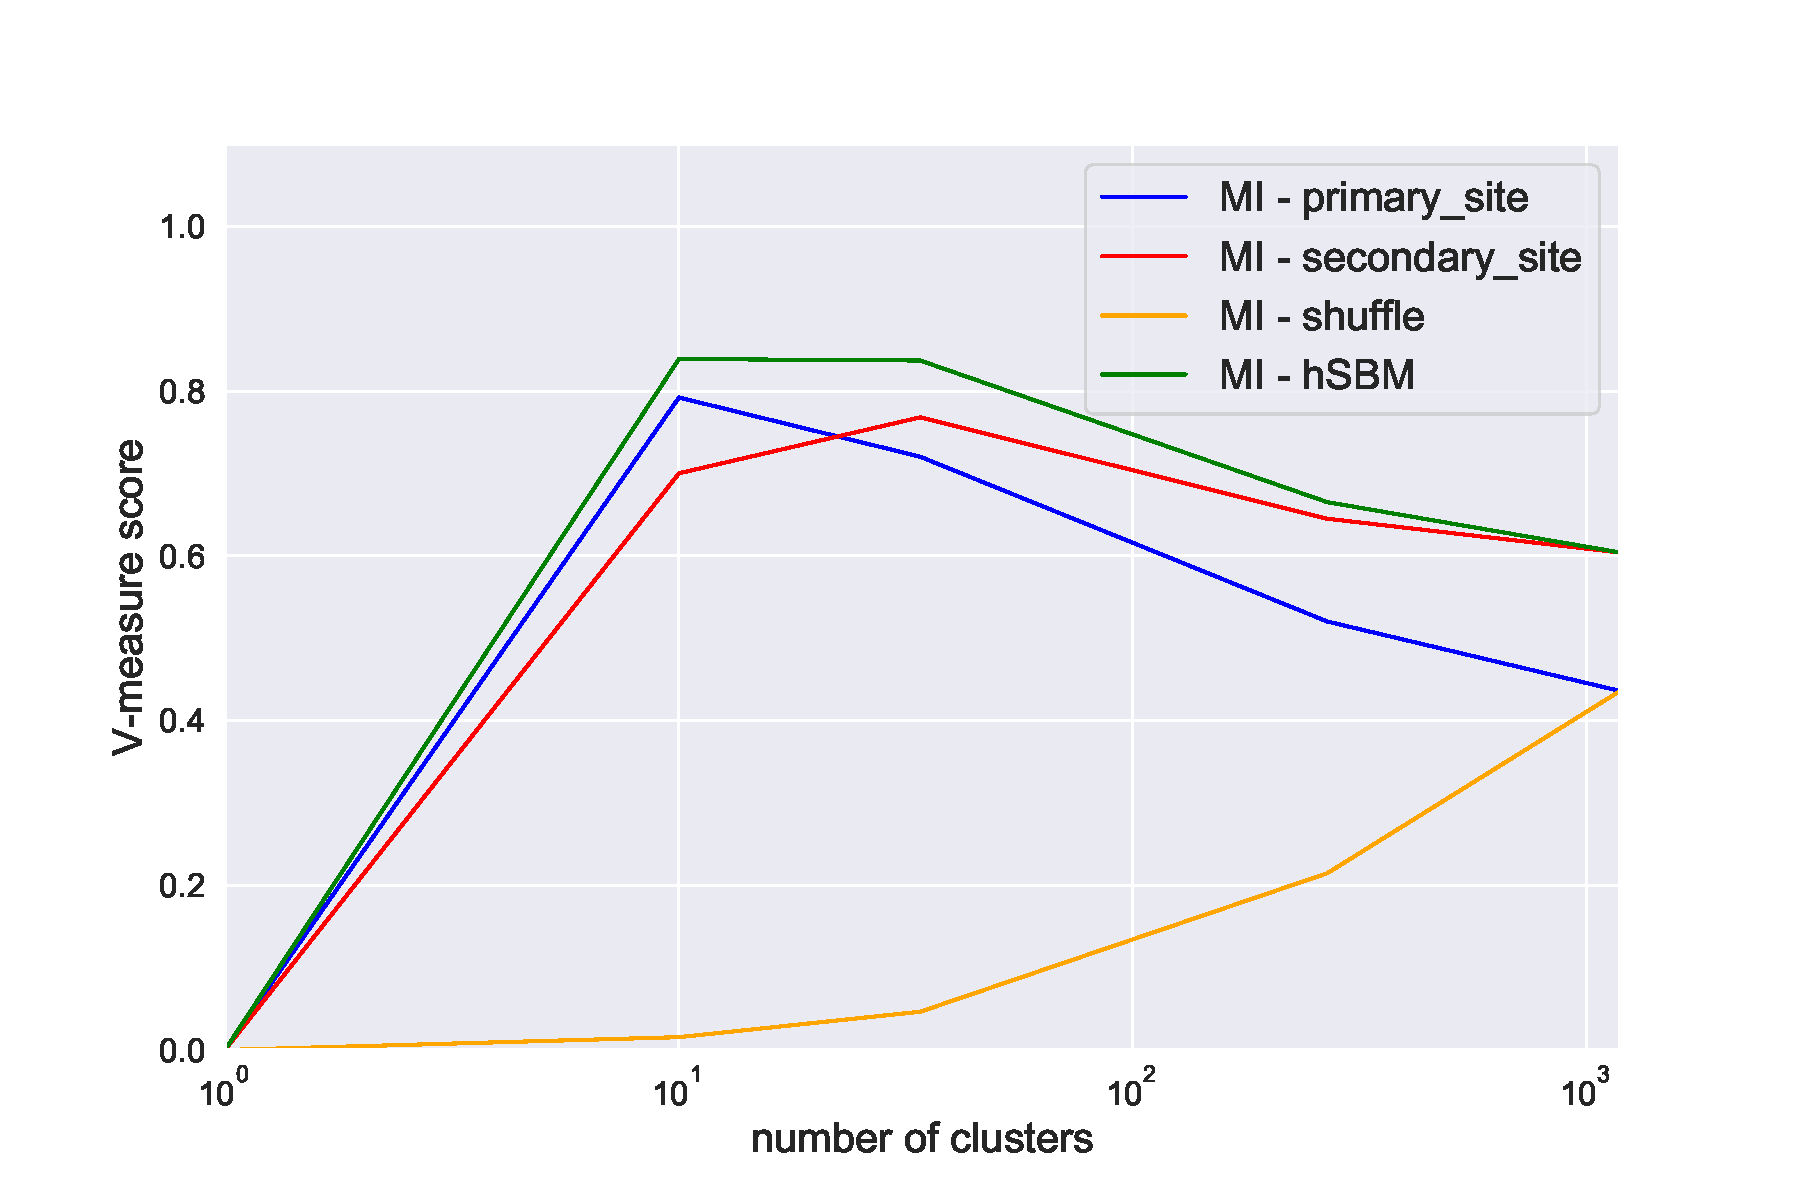
\includegraphics[width=0.9\linewidth]{pictures/topic/gtex/oversigma_10tissue/metric_scores_shuffle.pdf}
    \caption{Scores across the hierarchy. The scored is compared with some random labels. In blue the score for the primary site labels, in red for the secondary site labels, in yellow the shuffled labels, in green the mixed score with primary homogeneity and secondary completeness.}
    \label{fig:topic/gtex/oversigma_10tissue/metric_scores_shuffle}
\end{figure}
\FloatBarrier

\subsection{Comparison with standard algorithms}
At this point, it was verified that the model has got interesting output: it reaches high scores and has got a strong signal against the null model, at least at some levels of the hierarchy. It is now interesting to compare it with standard and well-studied similar algorithms.
First of all, a comparison is made with hierarchical clustering. This is done using the standard scipy package~\cite{jones2014scipy}, the metrics used was the euclidean one and the linkage method was set to Ward as briefly introduced in section~\ref{sec:hc}. This is quite fast, it needs a couple of minutes on a dual-core, 8GB memory machine.
In figure~\ref{fig:topic/gtex/oversigma_10tissue/metric_scores_hier} the comparison between these scores, the hierarchical algorithm performs worse than hierarchical Stochastic Block Model and as highly expected better than the random model.
\begin{figure}[htb!]
    \centering
    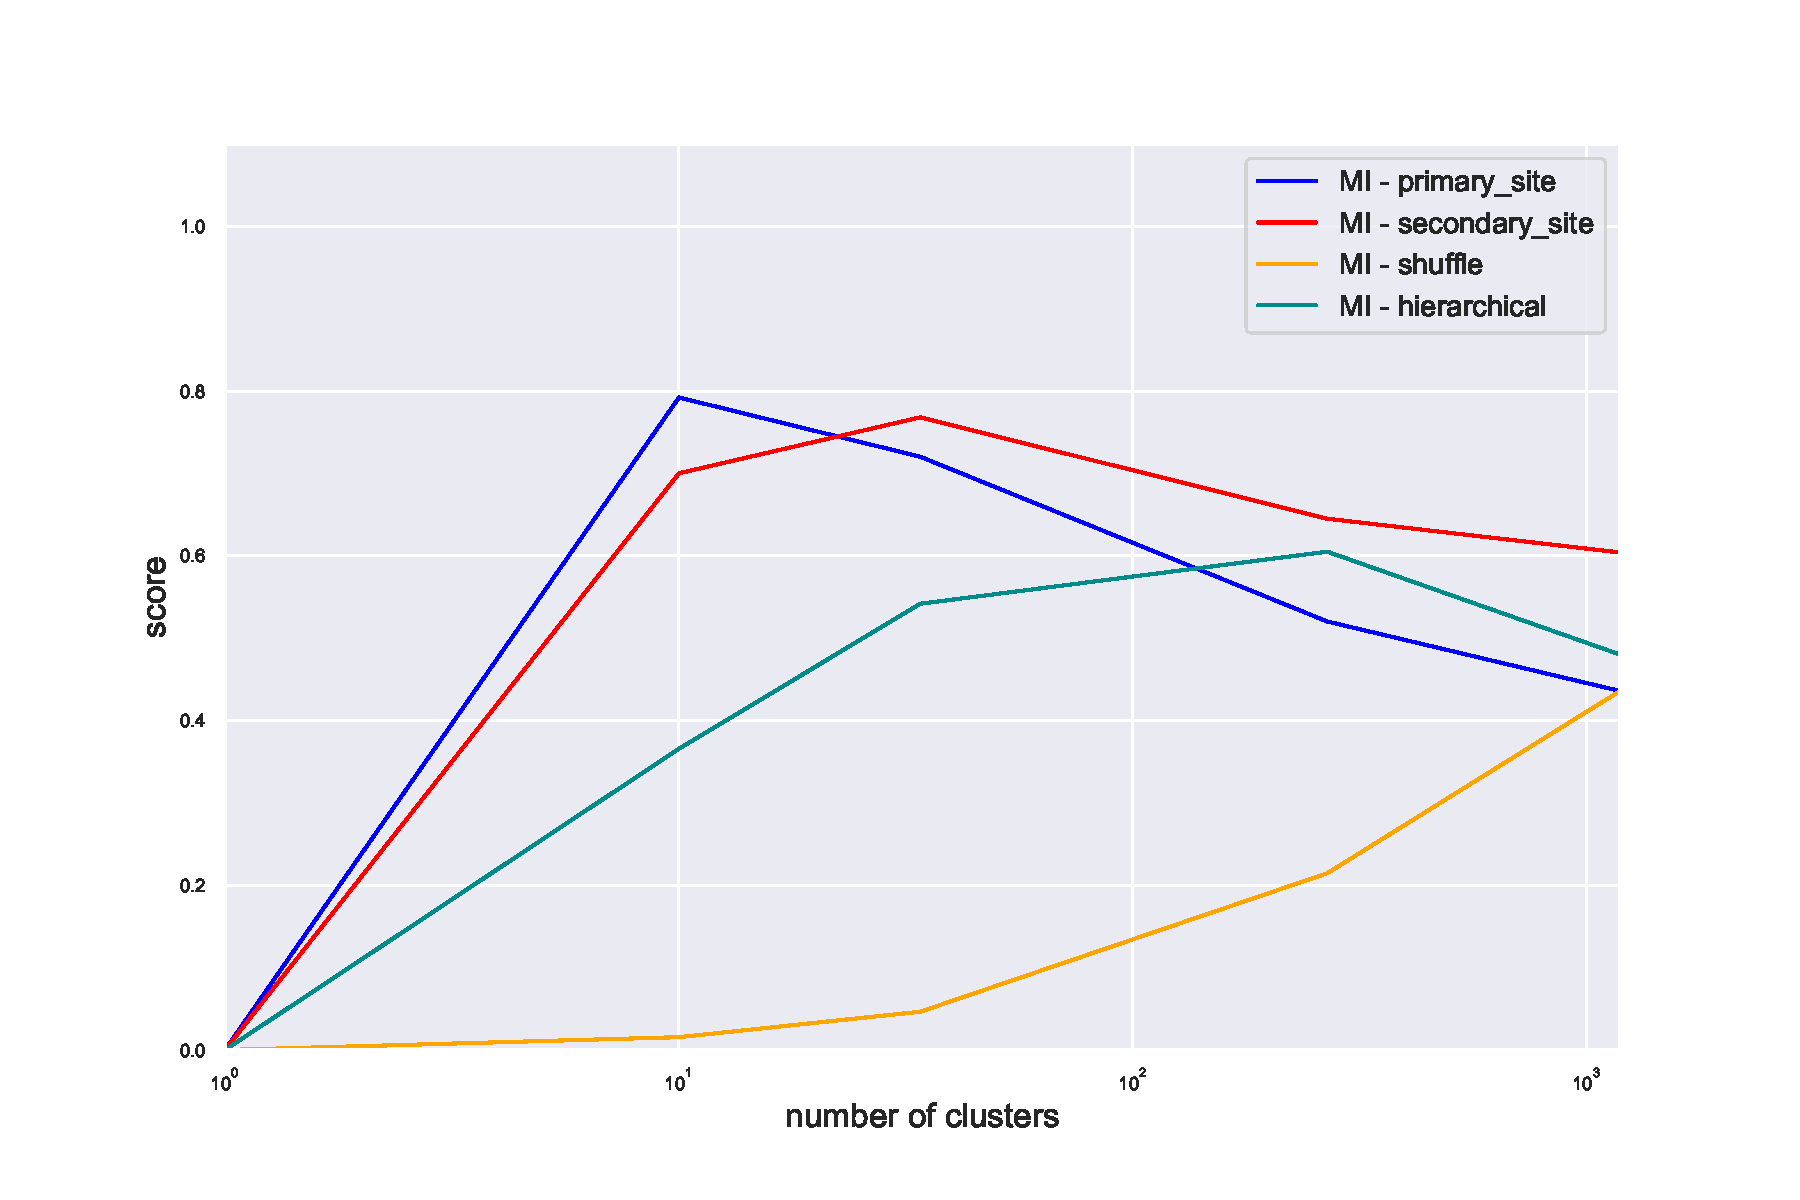
\includegraphics[width=0.9\linewidth]{pictures/topic/gtex/oversigma_10tissue/metric_scores_hier.pdf}
    \caption{Scores across the hierarchy. The score obtained with hSBM is compared with hierarchical clustering and shuffled labels.}
    \label{fig:topic/gtex/oversigma_10tissue/metric_scores_hier}
\end{figure}

Another very used and well-studied algorithm is Latent Dirichlet Allocation briefly described in~\ref{sec:lda}. Running LDA, as implemented standard scipy package, is quite fast and is comparable with hierarchical clustering in terms of CPU time. Note that once LDA package extracts the topics, it is necessary to define some clusters, to do so a standard Agglomerative clustering approach was used, the distance was set to \textit{euclidean} and the linkage to \textit{Ward}. In figure~\ref{fig:topic/gtex/oversigma_10tissue/metric_scores_all} the V-measure scores for all the algorithms described until this point are reported. It is clear that the hierarchical Stochastic Block Model performs better than all the others, LDA gains a little worse score and hierarchical clustering is the worst of the three. It is highly expected that all models are quite different from the random model. The fact that hSBM and LDA have higher scores suggests that a topic model approach can be very useful in this kind of problems. 
\begin{figure}[htb!]
    \centering
    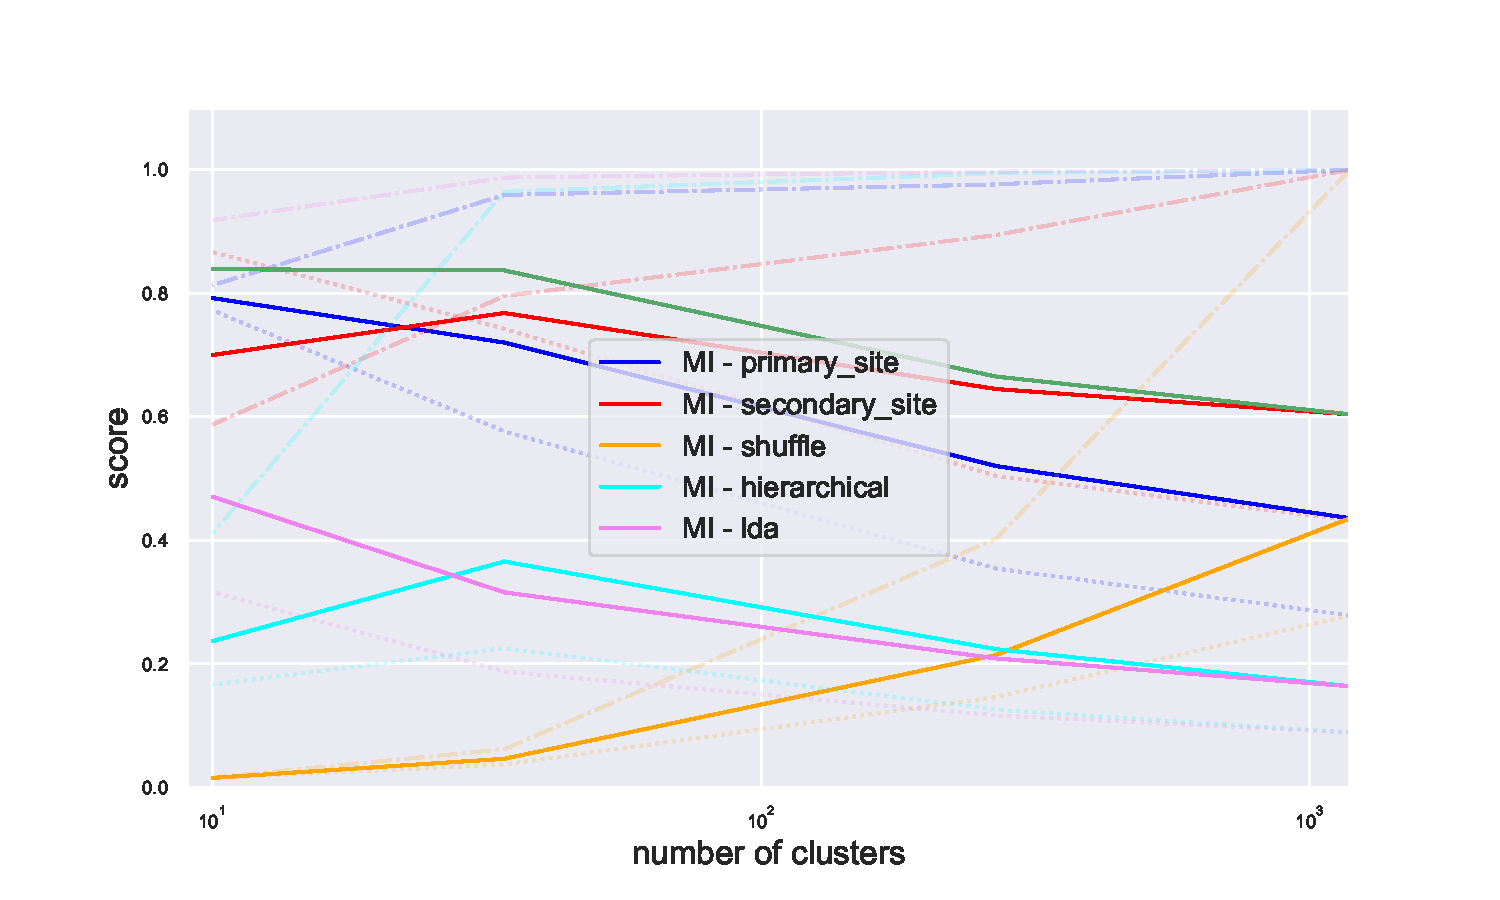
\includegraphics[width=0.9\linewidth]{pictures/topic/gtex/oversigma_10tissue/metric_scores_all.pdf}
    \caption{Scores across hierarchy for all algorithms used in this work.}
    \label{fig:topic/gtex/oversigma_10tissue/metric_scores_all}
\end{figure}
Note that LDA and hierarchical cluster models were not fine-tuned and default parameters were used. Maybe a fine-tuning of these packages can lead to better and more satisfying results. This analysis, considering that the comparison was made with hierarchical Stochastic Block Model which is non-parametric and needs no setting, was done without any fine-tuning and standard parameters were set. This fact reveals another good point of hSBM, it extracts not only better clusters, but also the parameters necessary to this kind of models. Moreover, the number of topics was set to the one obtained from hSBM; LDA is not able to select the number of topics.

\FloatBarrier
\subsection{Topics enrichment tests}
The analyses up to this point considered only one of the two sides of the bipartite network; nothing was told yet about the genes (words in topic models).
The model outputs some clusters of genes, though.  From now on these clusters of genes will be called topics.

If one has got a set of genes, it is possible to perform an enrichment test to catch any important information and discover if there are any biological meanings behind it. Enrichment analysis checks whether an input set of genes significantly overlaps with annotated gene sets.
In this work tests were made using Gene Set Enrichment Analysis (GSEA)~\cite{subramanian2005gene} python tool~\cite{Kuleshov2016}, which performs a Fisher exact test (hypergeometric test). The Benjamini-Hochberg adjusted P-values is reported. Genes' annotation terms were searched in the following sets: 
\begin{itemize}
		\item GO\footnote{Gene Ontology} Molecular Function 2018
		\item GO Biological Process 2018
		\item GO Cellular Component 2018
		\item Human Phenotype Ontology
		\item Tissue Protein Expression from Human Proteome Map
		\item KEGG 2019 Human
		\item NCI-60 Cancer Cell Lines
		\item GTEx Tissue Sample Gene Expression Profiles up
		\item GTEx Tissue Sample Gene Expression Profiles down,
\end{itemize}
in particular the two latter contain annotation specific for GTEx dataset~\cite{Ardlie2015}.

In tables~\ref{tab:topic/enrich/pancreas},~\ref{tab:topic/enrich/brain} and~\ref{tab:topic/enrich/blood} examples of enrichment test results. Each table is a topic by hSBM. On the results it is put a P-value cut at $0.05$ and terms are sorted by the adjusted P-value.
\begin{table}[htb!]
	\tiny
	\begin{center}
		\begin{tabular}{|l|c|r|}
			\hline
			Term & \multicolumn{1}{l|}{Adjusted P-value} & Gene set \\ \hline
			pancreas male 60-69 years & 1E-19 & GTEx Tissue Sample Gene Expression Profiles up \\ \hline
			pancreas female 40-49 years & 3E-19 & GTEx Tissue Sample Gene Expression Profiles up \\ \hline
			pancreas male 40-49 years & 5E-19 & GTEx Tissue Sample Gene Expression Profiles up \\ \hline
			pancreas male 30-39 years & 1E-18 & GTEx Tissue Sample Gene Expression Profiles up \\ \hline
			pancreas female 20-29 years & 1E-18 & GTEx Tissue Sample Gene Expression Profiles up \\ \hline
			pancreas male 50-59 years & 1E-18 & GTEx Tissue Sample Gene Expression Profiles up \\ \hline
			pancreas female 30-39 years & 1E-18 & GTEx Tissue Sample Gene Expression Profiles up \\ \hline
			pancreas male 50-59 years & 2E-18 & GTEx Tissue Sample Gene Expression Profiles up \\ \hline
			pancreas male 40-49 years & 2E-18 & GTEx Tissue Sample Gene Expression Profiles up \\ \hline
			pancreas male 30-39 years & 2E-18 & GTEx Tissue Sample Gene Expression Profiles up \\ \hline
			pancreas male 50-59 years & 2E-18 & GTEx Tissue Sample Gene Expression Profiles up \\ \hline
			pancreas female 20-29 years & 2E-18 & GTEx Tissue Sample Gene Expression Profiles up \\ \hline
			pancreas male 40-49 years & 3E-18 & GTEx Tissue Sample Gene Expression Profiles up \\ \hline
			pancreas female 50-59 years & 4E-18 & GTEx Tissue Sample Gene Expression Profiles up \\ \hline
			pancreas male 50-59 years & 4E-18 & GTEx Tissue Sample Gene Expression Profiles up \\ \hline
			pancreas male 50-59 years & 4E-18 & GTEx Tissue Sample Gene Expression Profiles up \\ \hline
			pancreas female 60-69 years & 5E-18 & GTEx Tissue Sample Gene Expression Profiles up \\ \hline
			pancreas female 50-59 years & 5E-18 & GTEx Tissue Sample Gene Expression Profiles up \\ \hline
			pancreas male 50-59 years & 5E-18 & GTEx Tissue Sample Gene Expression Profiles up \\ \hline
			pancreas male 30-39 years & 6E-18 & GTEx Tissue Sample Gene Expression Profiles up \\ \hline
		\end{tabular}
	\end{center}
	\caption{Enrichment test of a topic. It is clear the enrichment for pancreas-related gene sets.}
	\label{tab:topic/enrich/pancreas}
\end{table}
\begin{table}[htb!]
	\tiny
	\begin{center}
		\begin{tabular}{|l|c|r|}
			\hline
			Term & \multicolumn{1}{l|}{Adjusted P-value} & Gene set \\ \hline
			brain female 40-49 years & 6E-05 & GTEx Tissue Sample Gene Expression Profiles up \\ \hline
			brain male 50-59 years & 6E-05 & GTEx Tissue Sample Gene Expression Profiles up \\ \hline
			brain female 60-69 years & 6E-05 & GTEx Tissue Sample Gene Expression Profiles up \\ \hline
			brain female 60-69 years & 6E-05 & GTEx Tissue Sample Gene Expression Profiles up \\ \hline
			brain female 60-69 years & 6E-05 & GTEx Tissue Sample Gene Expression Profiles up \\ \hline
			brain female 40-49 years & 6E-05 & GTEx Tissue Sample Gene Expression Profiles up \\ \hline
			brain female 40-49 years & 6E-05 & GTEx Tissue Sample Gene Expression Profiles up \\ \hline
			brain female 60-69 years & 6E-05 & GTEx Tissue Sample Gene Expression Profiles up \\ \hline
			brain male 60-69 years & 6E-05 & GTEx Tissue Sample Gene Expression Profiles up \\ \hline
			brain male 50-59 years & 6E-05 & GTEx Tissue Sample Gene Expression Profiles up \\ \hline
			brain male 50-59 years & 6E-05 & GTEx Tissue Sample Gene Expression Profiles up \\ \hline
			brain male 60-69 years & 7E-05 & GTEx Tissue Sample Gene Expression Profiles up \\ \hline
			brain male 50-59 years & 7E-05 & GTEx Tissue Sample Gene Expression Profiles up \\ \hline
			brain male 20-29 years & 7E-05 & GTEx Tissue Sample Gene Expression Profiles up \\ \hline
			brain female 60-69 years & 8E-05 & GTEx Tissue Sample Gene Expression Profiles up \\ \hline
			brain female 60-69 years & 8E-05 & GTEx Tissue Sample Gene Expression Profiles up \\ \hline
			brain female 60-69 years & 1E-04 & GTEx Tissue Sample Gene Expression Profiles up \\ \hline
			brain female 60-69 years & 1E-04 & GTEx Tissue Sample Gene Expression Profiles up \\ \hline
			brain female 60-69 years & 1E-04 & GTEx Tissue Sample Gene Expression Profiles up \\ \hline
			brain male 60-69 years & 1E-04 & GTEx Tissue Sample Gene Expression Profiles up \\ \hline
		\end{tabular}
	\end{center}
	\caption{Enrichment test of a topic. It is clear the enrichment for brain-related gene sets.}
	\label{tab:topic/enrich/brain}
\end{table}
\begin{table}[htb!]
	\centering
	\tiny
	\begin{tabular}{|l|c|r|}
		\hline
		Term & \multicolumn{1}{l|}{Adjusted P-value} & Gene set \\ \hline
		blood male 50-59 years & 3E-23 & GTEx Tissue Sample Gene Expression Profiles up \\ \hline
		blood male 50-59 years & 3E-23 & GTEx Tissue Sample Gene Expression Profiles up \\ \hline
		blood male 40-49 years & 3E-21 & GTEx Tissue Sample Gene Expression Profiles up \\ \hline
		blood male 60-69 years & 9E-21 & GTEx Tissue Sample Gene Expression Profiles up \\ \hline
		blood male 40-49 years & 3E-20 & GTEx Tissue Sample Gene Expression Profiles up \\ \hline
		blood female 60-69 years & 4E-20 & GTEx Tissue Sample Gene Expression Profiles up \\ \hline
		blood male 60-69 years & 4E-20 & GTEx Tissue Sample Gene Expression Profiles up \\ \hline
		blood female 50-59 years & 5E-20 & GTEx Tissue Sample Gene Expression Profiles up \\ \hline
		blood female 50-59 years & 1E-19 & GTEx Tissue Sample Gene Expression Profiles up \\ \hline
		blood male 60-69 years & 1E-19 & GTEx Tissue Sample Gene Expression Profiles up \\ \hline
		blood male 60-69 years & 1E-19 & GTEx Tissue Sample Gene Expression Profiles up \\ \hline
		blood female 60-69 years & 1E-19 & GTEx Tissue Sample Gene Expression Profiles up \\ \hline
		blood male 60-69 years & 2E-19 & GTEx Tissue Sample Gene Expression Profiles up \\ \hline
		blood male 50-59 years & 2E-19 & GTEx Tissue Sample Gene Expression Profiles up \\ \hline
		blood female 40-49 years & 2E-19 & GTEx Tissue Sample Gene Expression Profiles up \\ \hline
		blood female 40-49 years & 2E-19 & GTEx Tissue Sample Gene Expression Profiles up \\ \hline
		blood female 60-69 years & 2E-19 & GTEx Tissue Sample Gene Expression Profiles up \\ \hline
		blood male 30-39 years & 3E-19 & GTEx Tissue Sample Gene Expression Profiles up \\ \hline
		blood female 50-59 years & 5E-19 & GTEx Tissue Sample Gene Expression Profiles up \\ \hline
		blood female 60-69 years & 5E-19 & GTEx Tissue Sample Gene Expression Profiles up \\ \hline
	\end{tabular}
	\caption{Enrichment test of a topic. It is clear the enrichment for blood-related gene sets.}
		\label{tab:topic/enrich/blood}
\end{table}
Tests were made on the topics at the level of the hierarchy which obtained the higher V-measure score on the sample side of the network. These results are very interesting, these enrichment tests demonstrate that not only the sample side of the network is well clustered but also the topics have a non-trivial meaning.

So also the topics are related to the tissues and somehow are tissue-specific. In the next examples, the relationship between the topics and the samples will be further investigated. In particular following what was done by~\cite{dey2017visualizing} the importance of each topic inside each sample, the $P(\text{topic} | \text{sample})$, will be discussed.

\FloatBarrier
Separate healthy tissues is a good exercise and a good benchmark for models, but the real goals would be being able to classify diseased samples. It is not always easy to identify and classify cancer tissues. In particular, being able to separate tumour sub-types would be the ideal pursuance of this work. So let's switch to the analysis of diseased samples.

%%tcga
\clearpage
\subsection{Run on TCGA}
Confirms that~\ref{fig:structure/tcga/fraction_of_trascriptome_disease}

\begin{figure}[htb!]
    \centering
    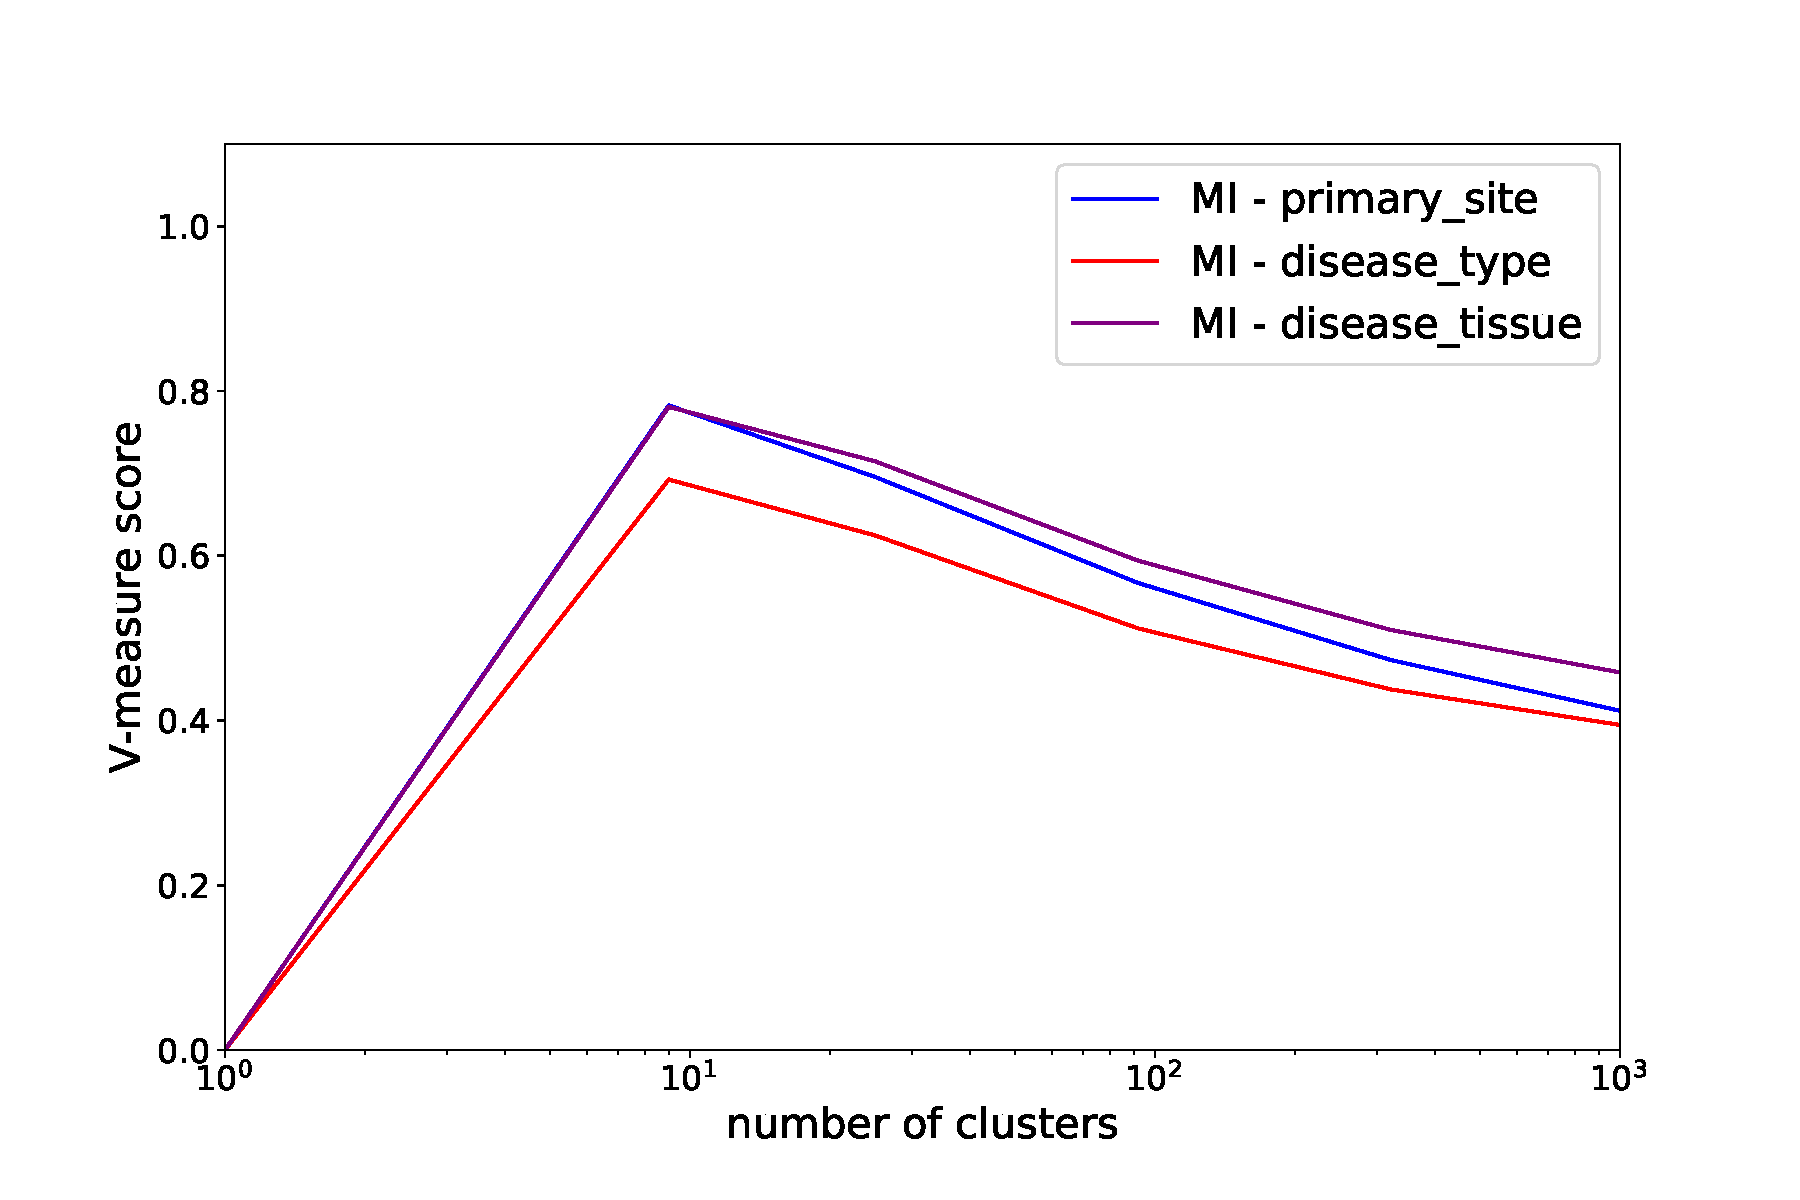
\includegraphics[width=0.8\linewidth]{pictures/topic/tcga/metric.pdf}
    \caption{\draft{tumori più difficile}}
    \label{fig:topic/tcga/metric}
\end{figure}

\begin{figure}[htb!]
	\centering
	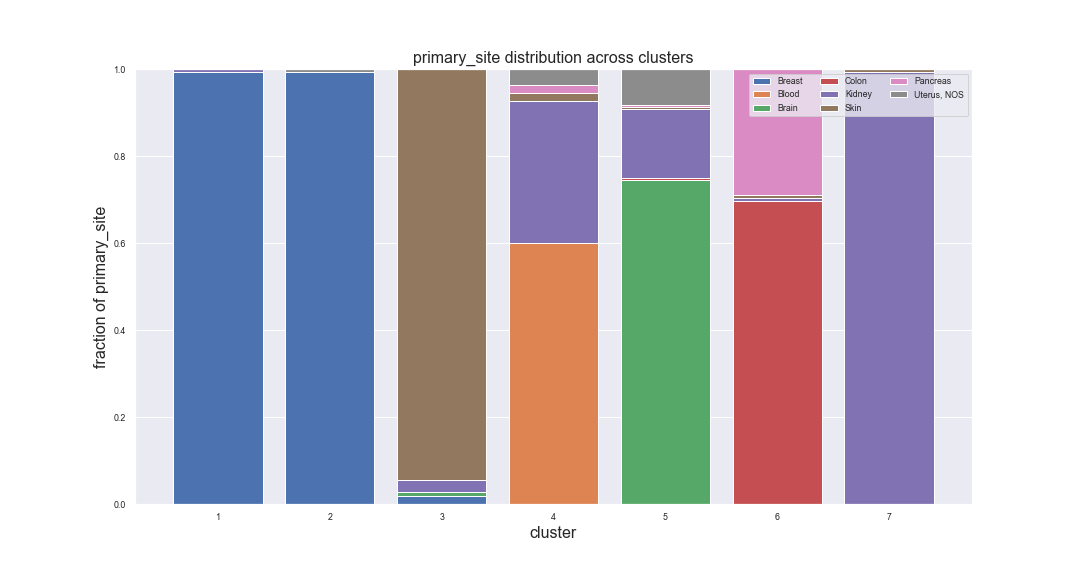
\includegraphics[width=0.8\linewidth]{pictures/topic/tcga/fraction_clustercomposition_l4_primary_site.png}
	\caption{text}
	\label{fig:topic/tcga/fraction_clustercomposition_l4_primary_site}
\end{figure}

\begin{figure}[htb!]
	\centering
	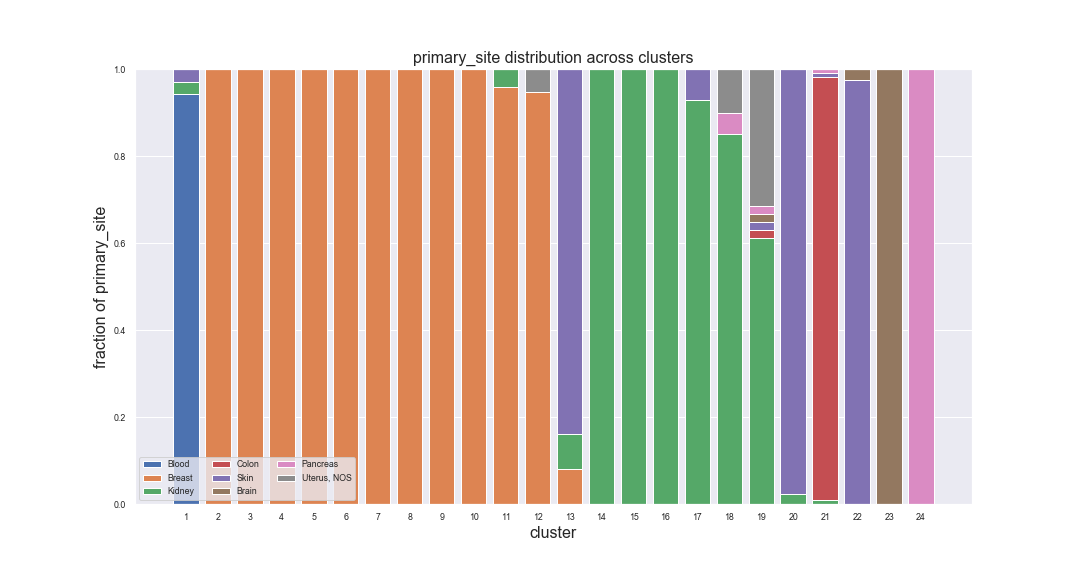
\includegraphics[width=0.8\linewidth]{pictures/topic/tcga/fraction_clustercomposition_l3_primary_site.png}
	\caption{text}
	\label{fig:topic/tcga/fraction_clustercomposition_l3_primary_site}
\end{figure}

\clearpage
\subsection{Mixed runs}
Getting normalised data from~\cite{Betel2018} available as a dataset~\cite{Wang2017}. it is possible to analyse health and diseased at the same time.

It is 
\begin{figure}[htb!]
    \centering
    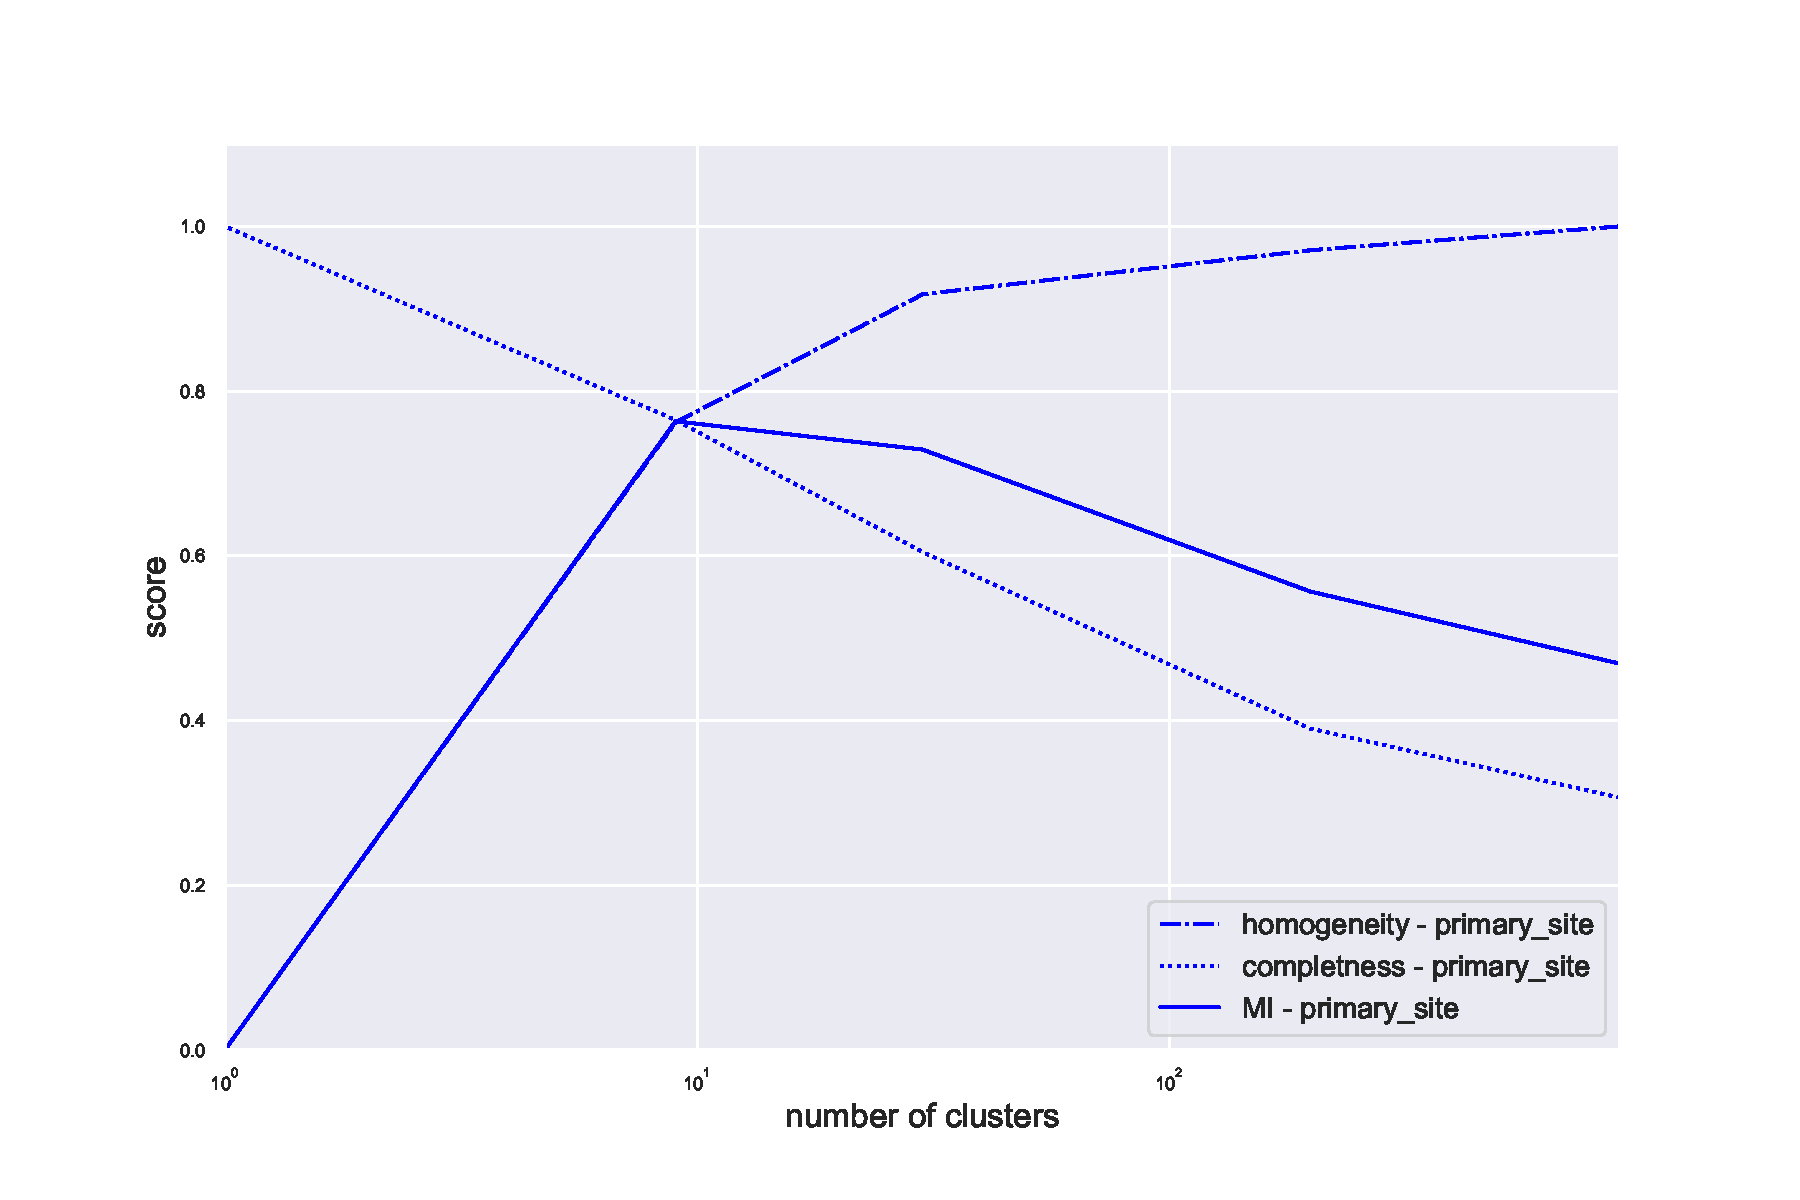
\includegraphics[width=0.8\linewidth]{pictures/topic/merged/metric_scores_primarysite.pdf}
    \caption{Caption}
    \label{fig:topic/merged/metric_scores_primarysite}
\end{figure}

\begin{figure}[htb!]
    \centering
    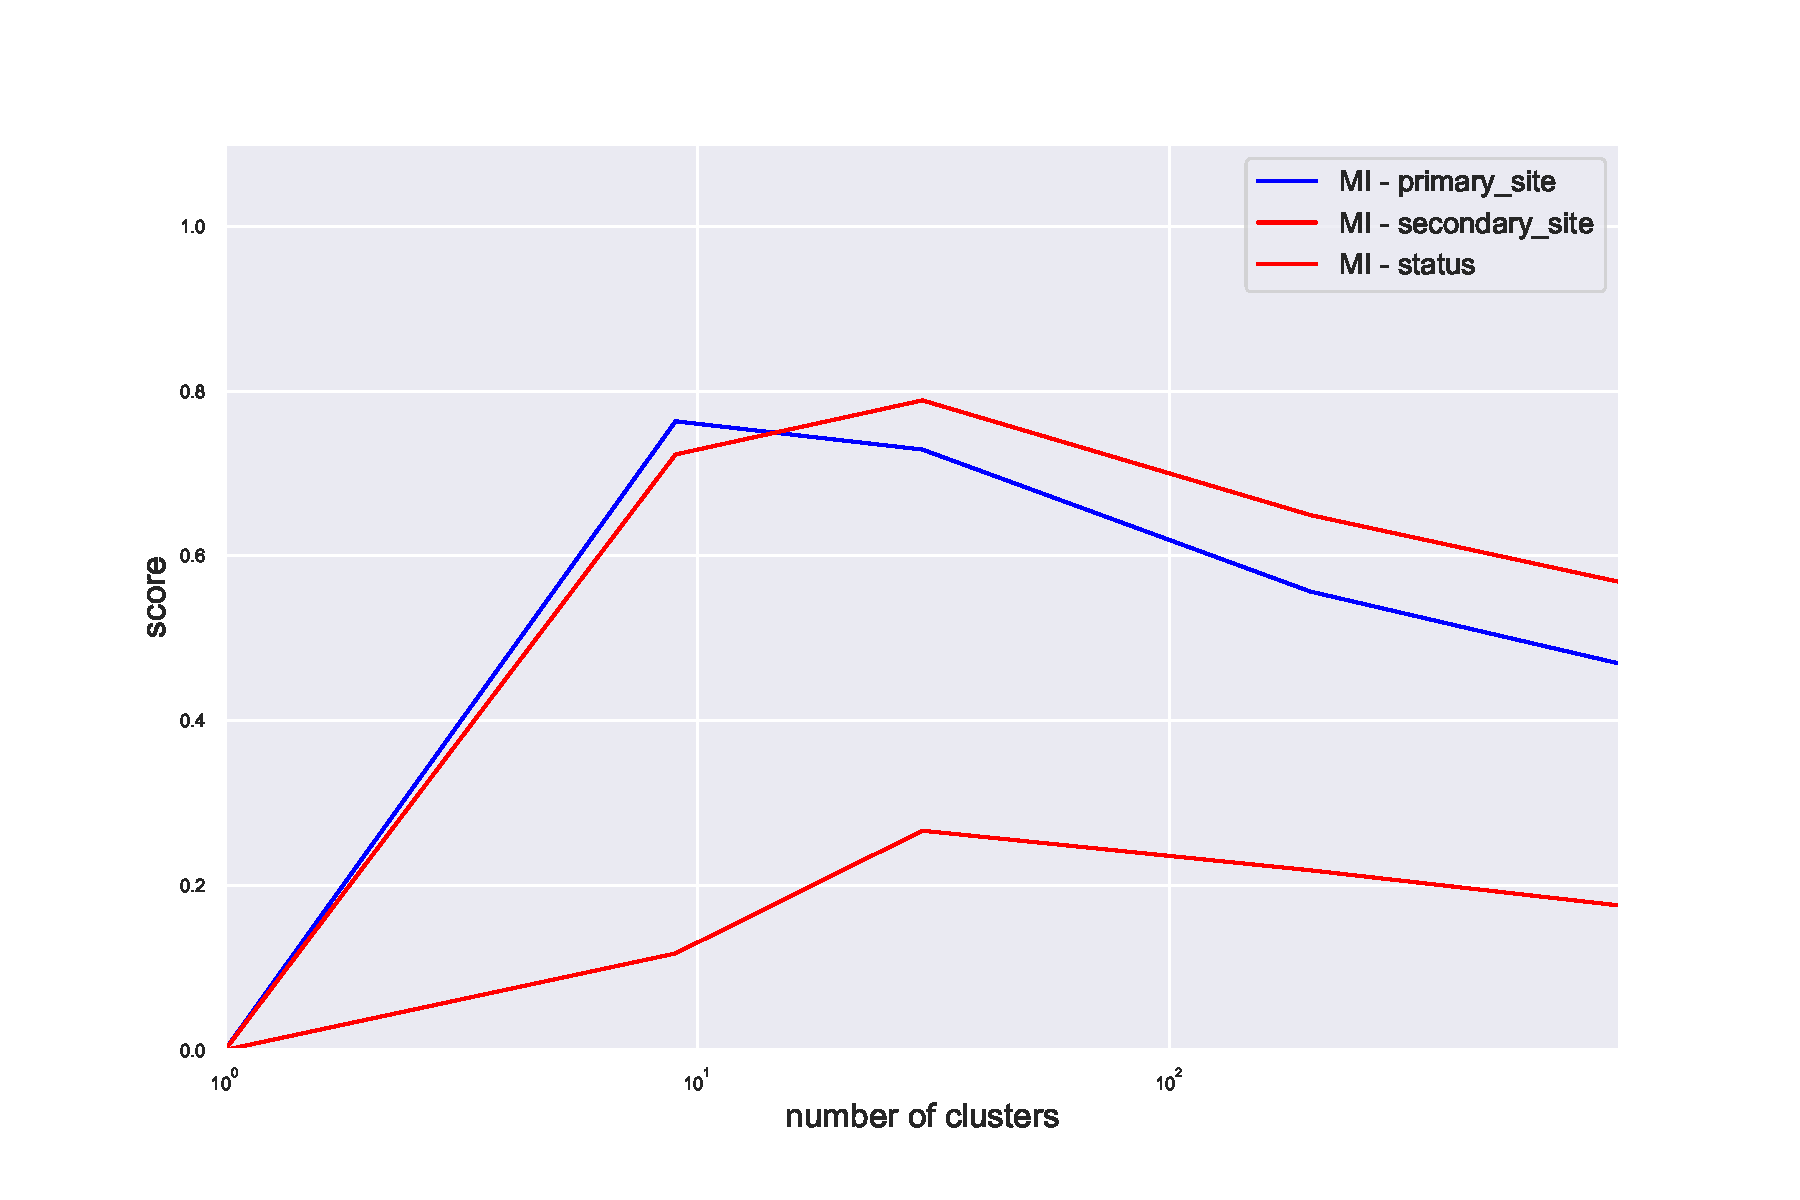
\includegraphics[width=0.8\linewidth]{pictures/topic/merged/metric_scores.pdf}
    \caption{Caption}
    \label{fig:topic/merged/metric_scores}
\end{figure}

\begin{figure}[htb!]
    \centering
    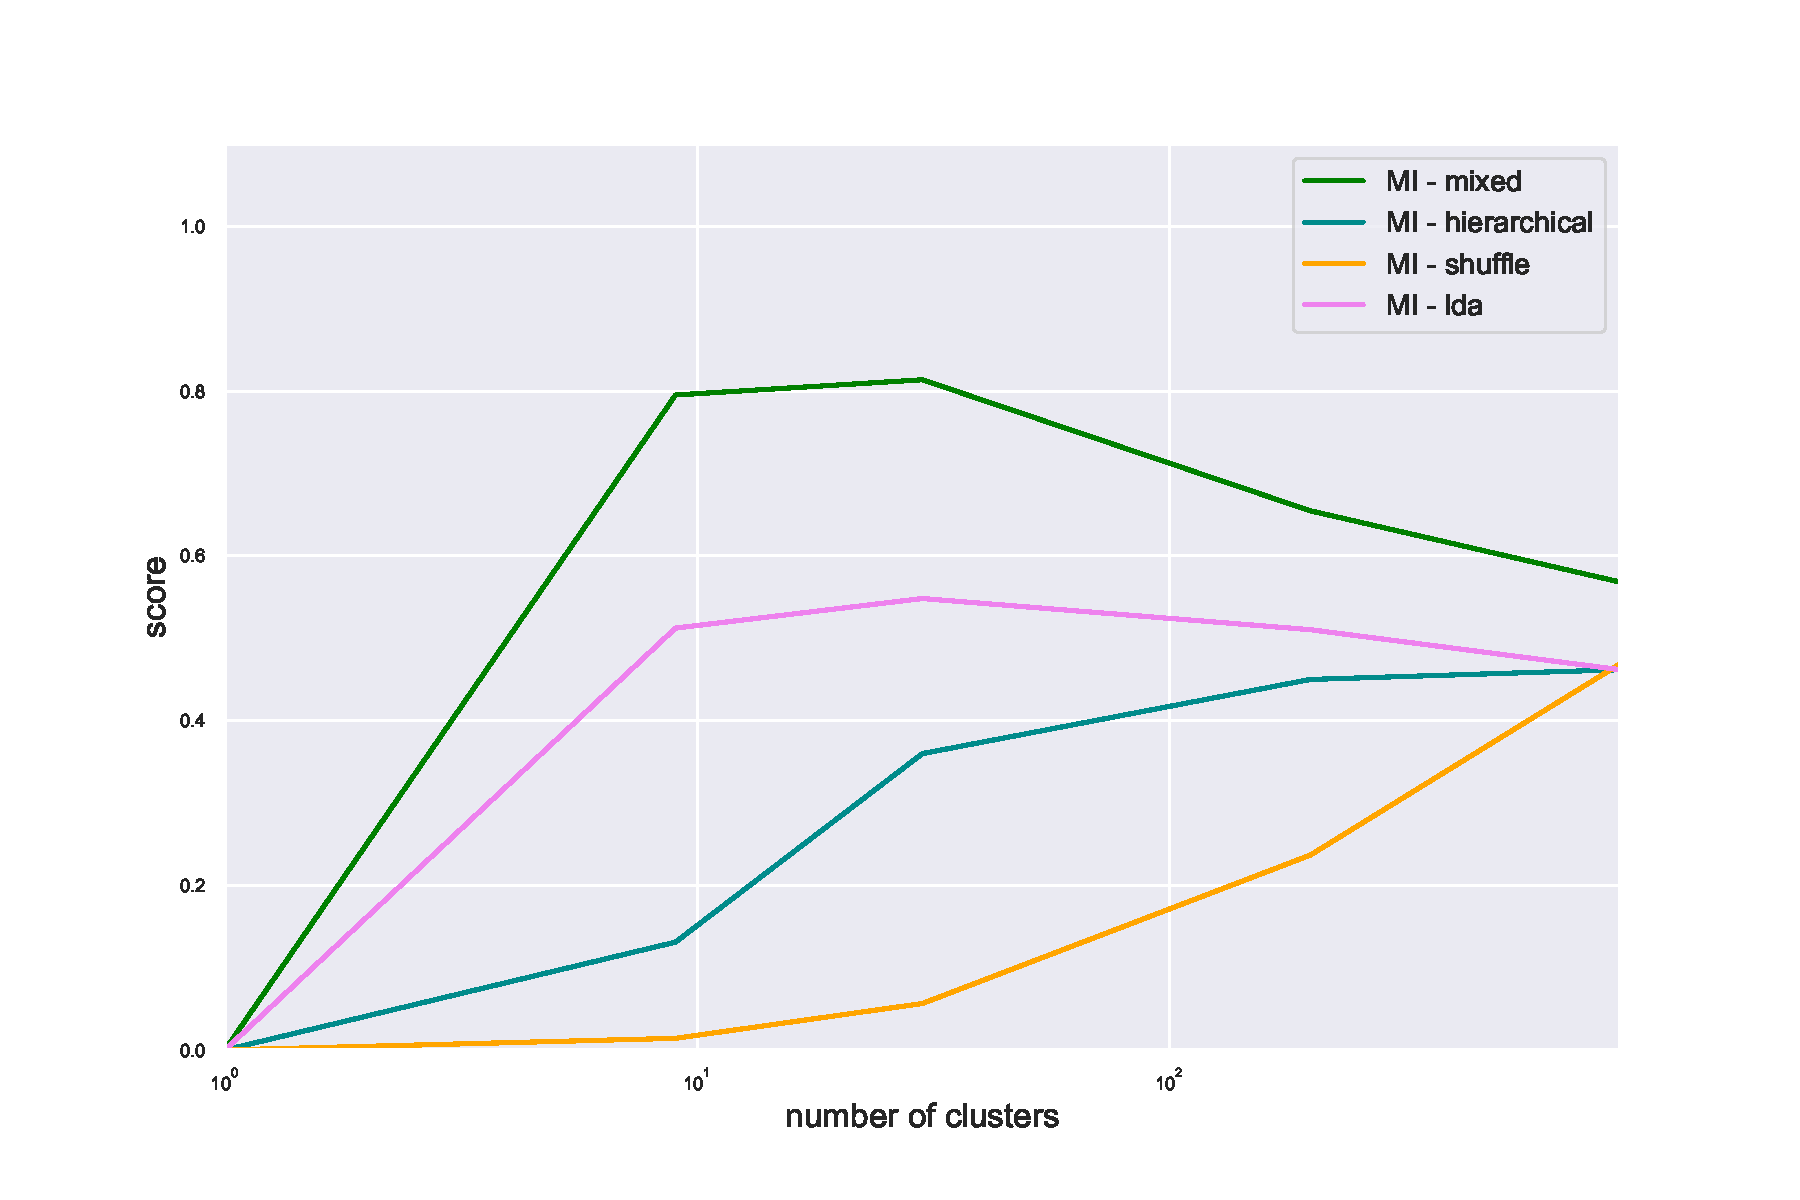
\includegraphics[width=0.8\linewidth]{pictures/topic/merged/metric_scores_all.pdf}
    \caption{Caption}
    \label{fig:topic/merged/metric_scores_all}
\end{figure}

\begin{figure}[htb!]
    \centering
    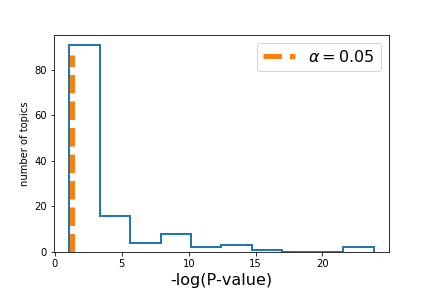
\includegraphics[width=0.8\linewidth]{pictures/topic/merged/pvaluescrosstopic.png}
    \caption{Caption}
    \label{fig:topic/merged/pvaluescrosstopic}
\end{figure}


\begin{figure}[htb!]
    \centering
    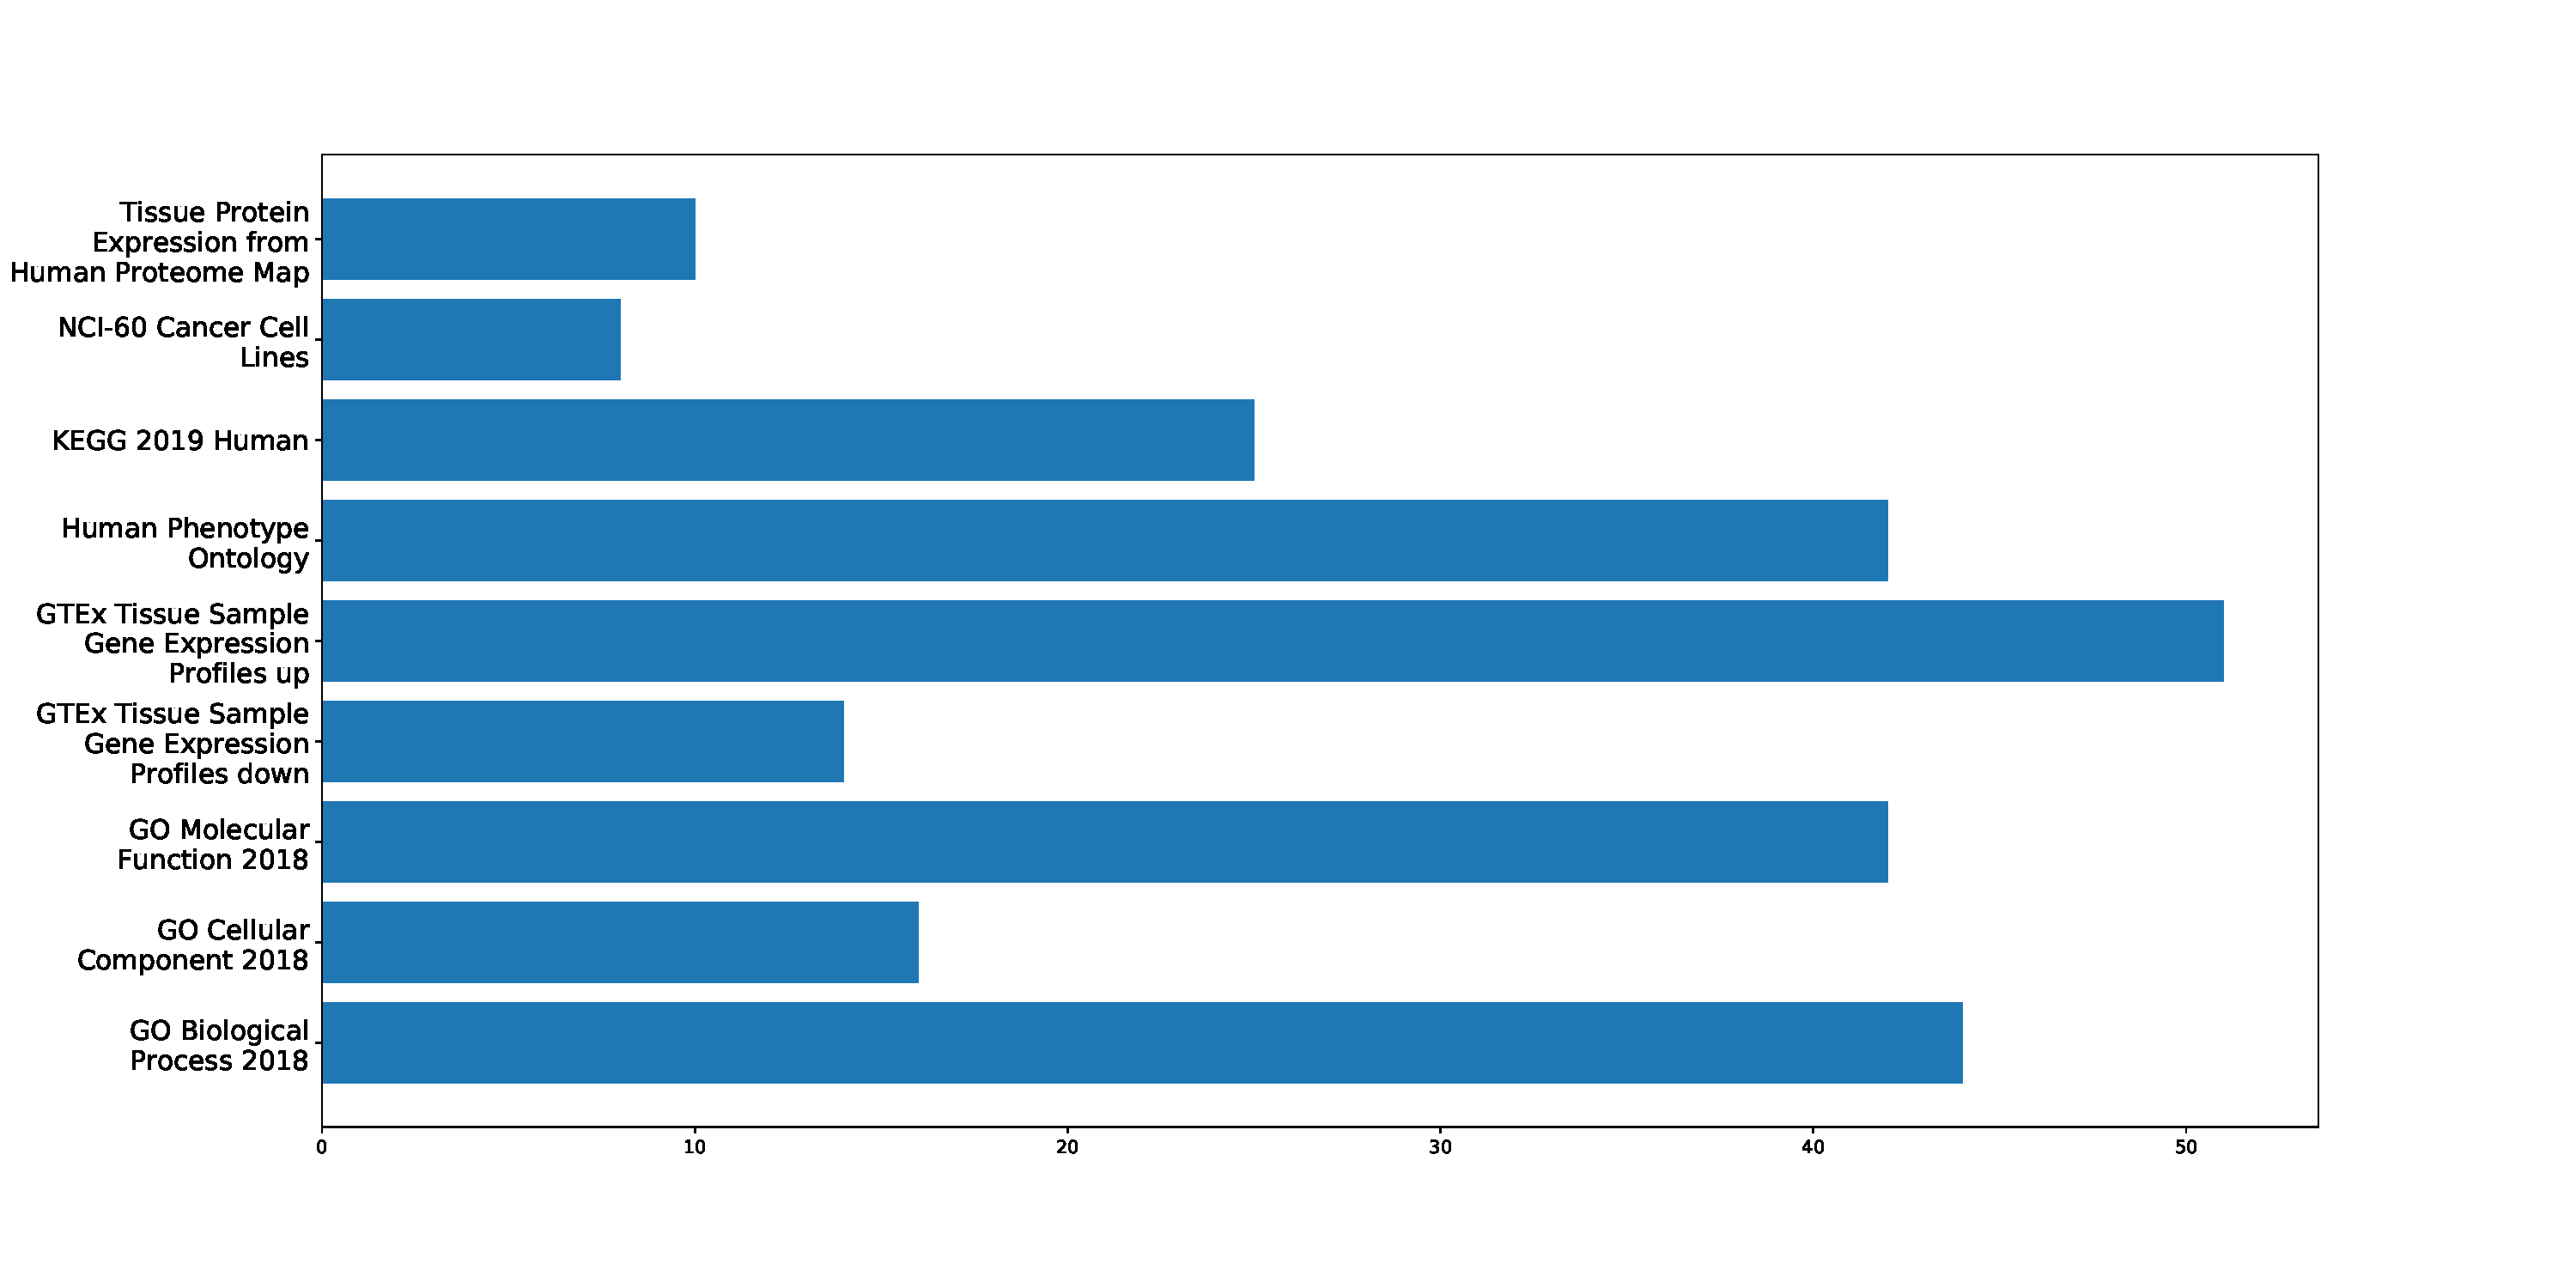
\includegraphics[width=0.8\linewidth]{pictures/topic/merged/pvaluecategories.pdf}
    \caption{Caption}
    \label{fig:topic/merged/pvaluecategories}
\end{figure}

DAVID~\cite{huang2008bioinformatics,huang2009systematic} confirms analogous result
\begin{figure}[htb!]
    \centering
    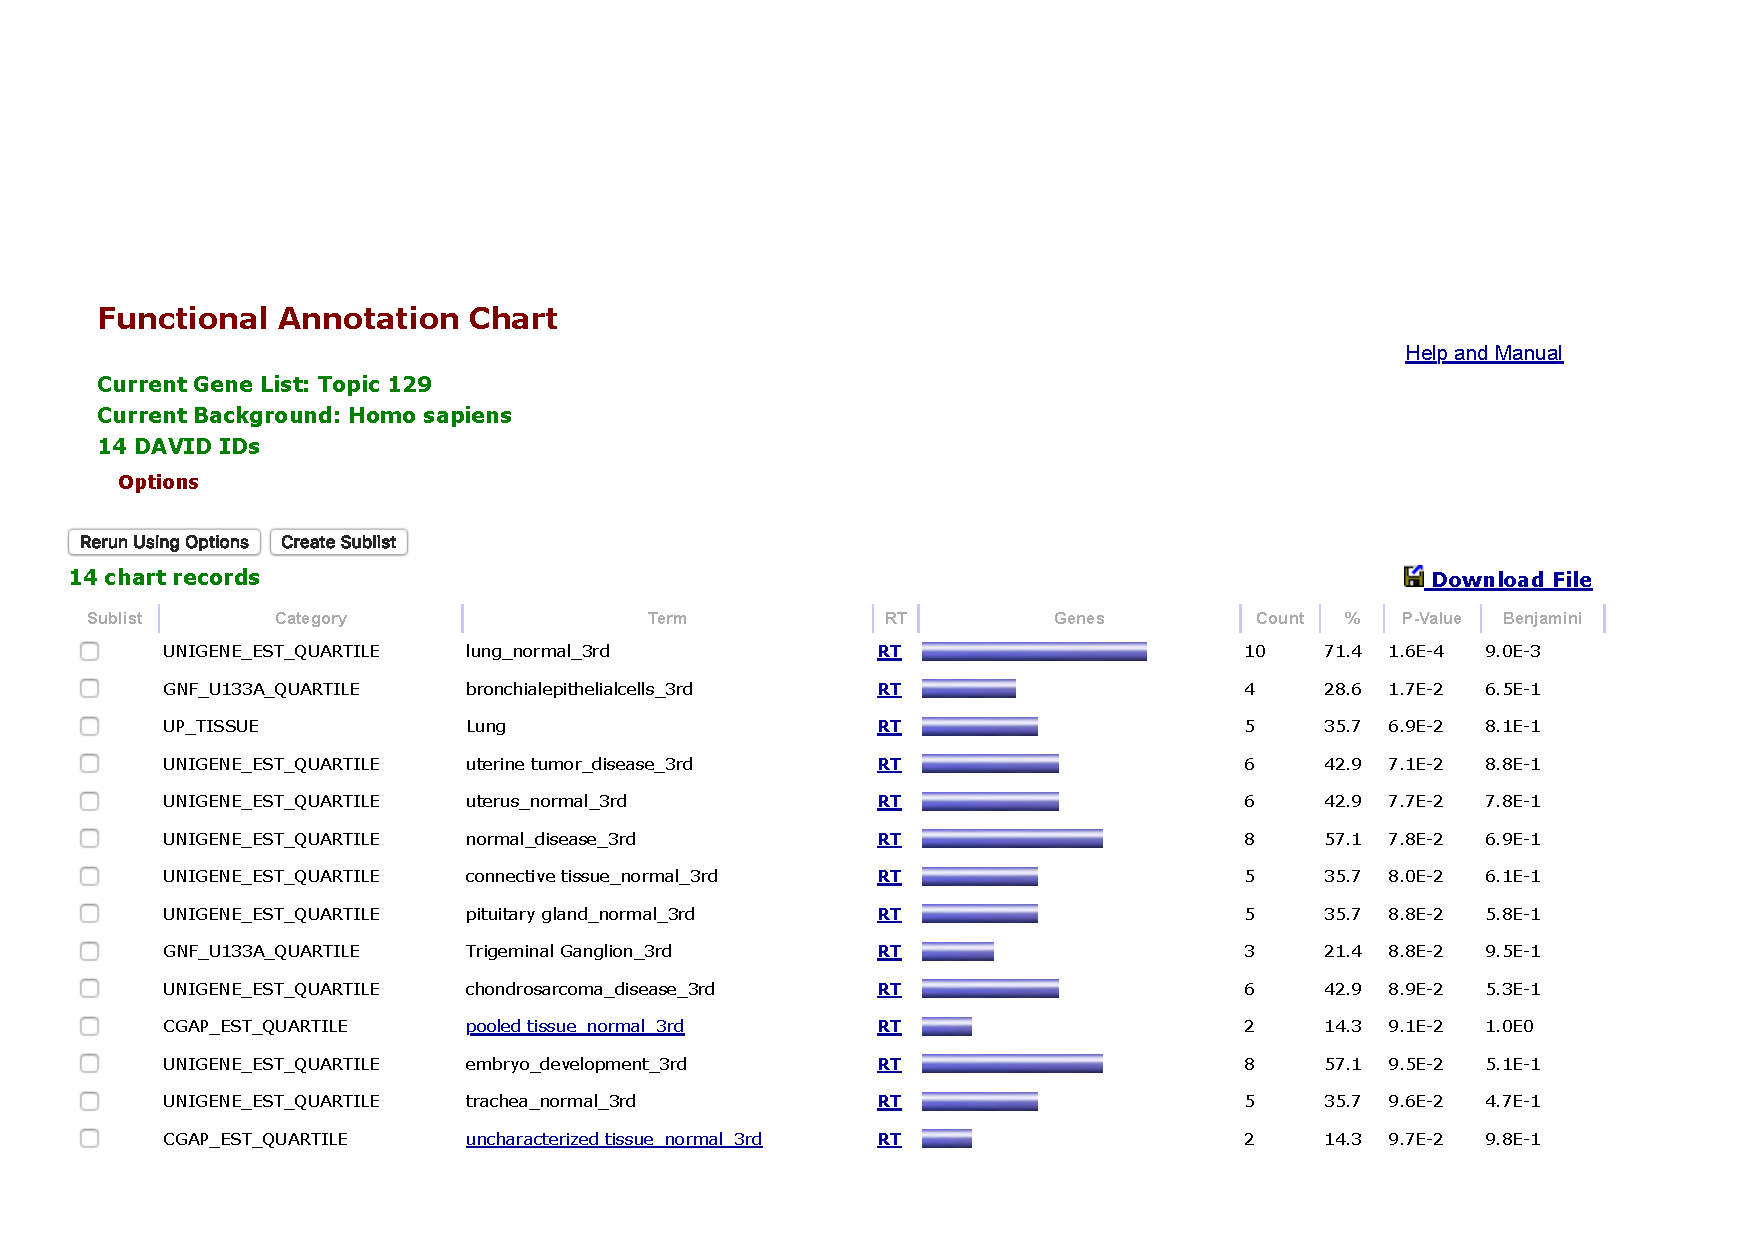
\includegraphics[width=0.8\linewidth]{pictures/topic/merged/DAVID_lung.pdf}
    \caption{Caption}
    \label{fig:topic/merged/DAVID_lung}
\end{figure}

\begin{figure}[htb!]
    \centering
    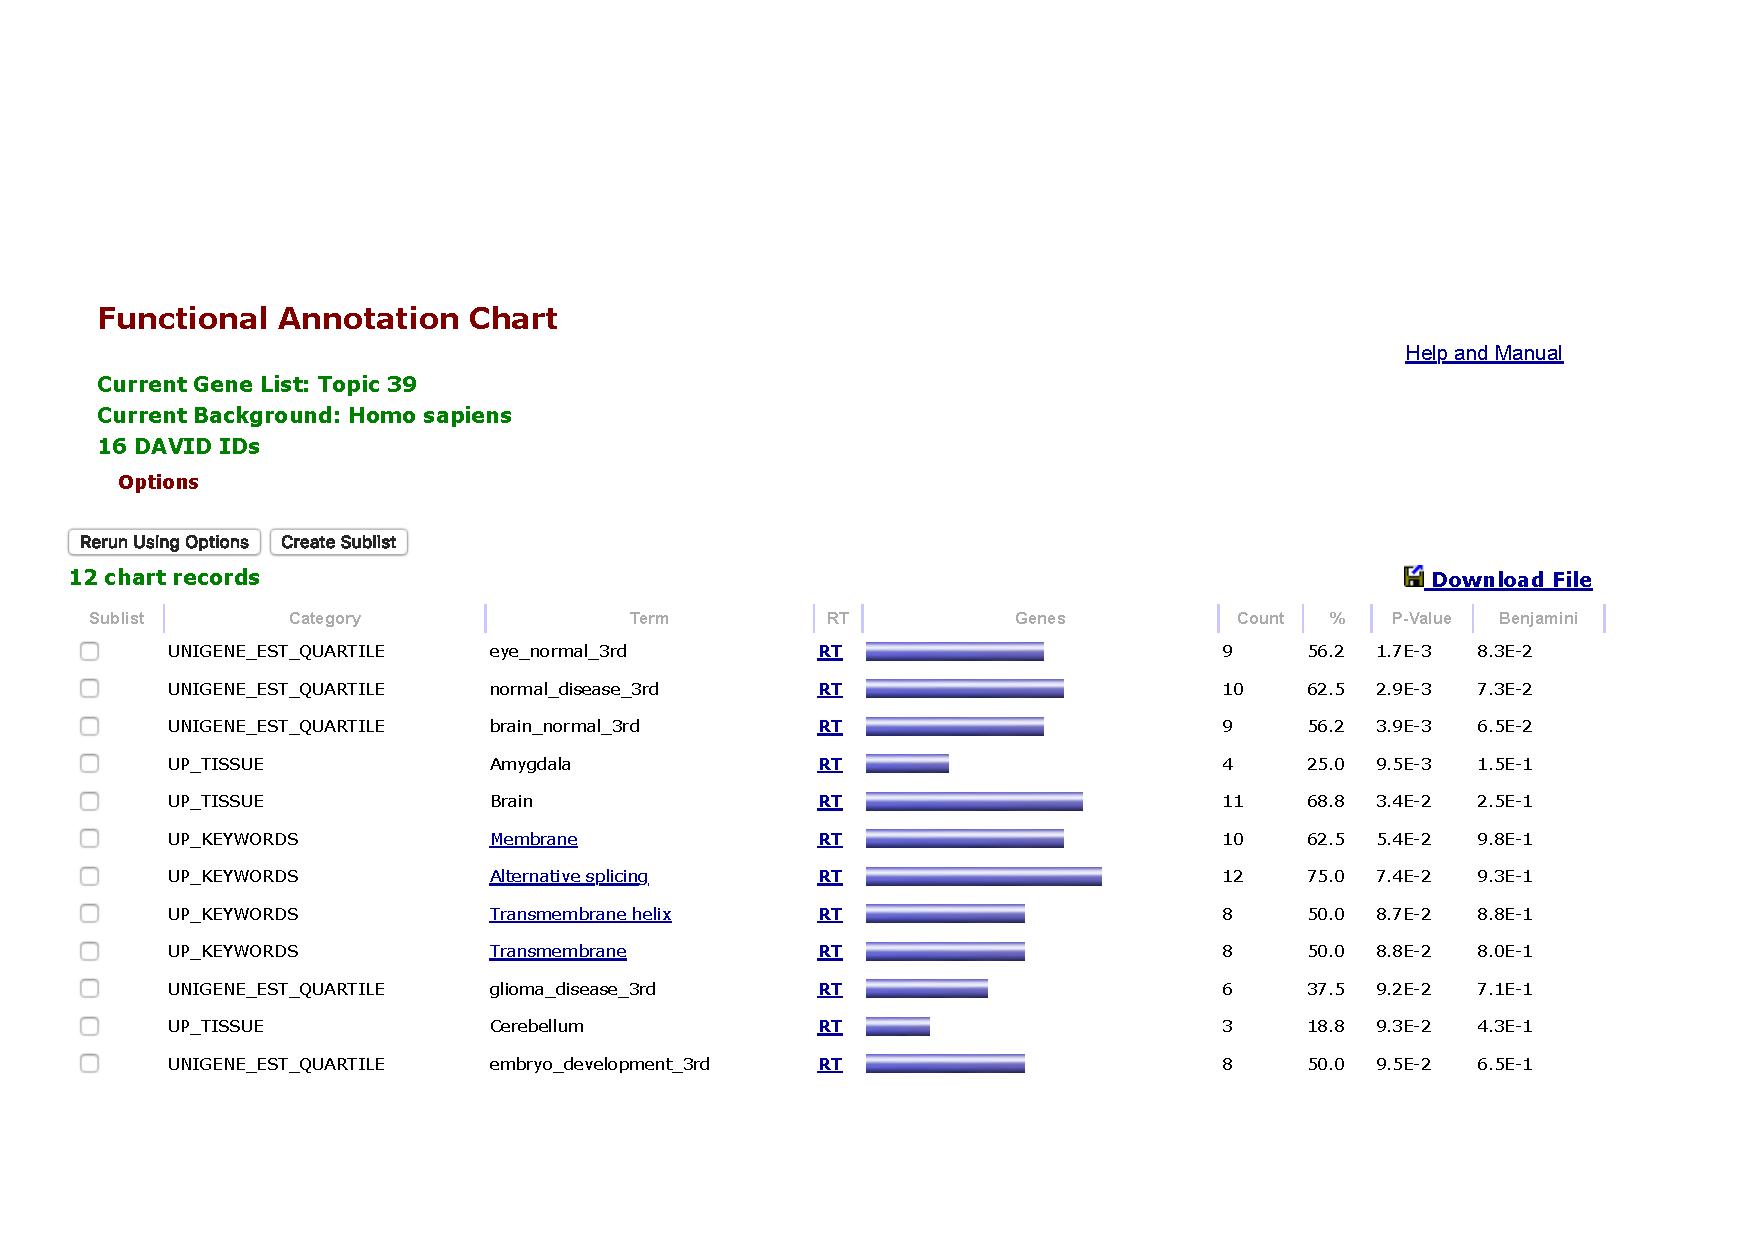
\includegraphics[width=0.8\linewidth]{pictures/topic/merged/DAVID_brain.pdf}
    \caption{Caption}
    \label{fig:topic/merged/DAVID_brain}
\end{figure}

\begin{figure}[htb!]
    \centering
    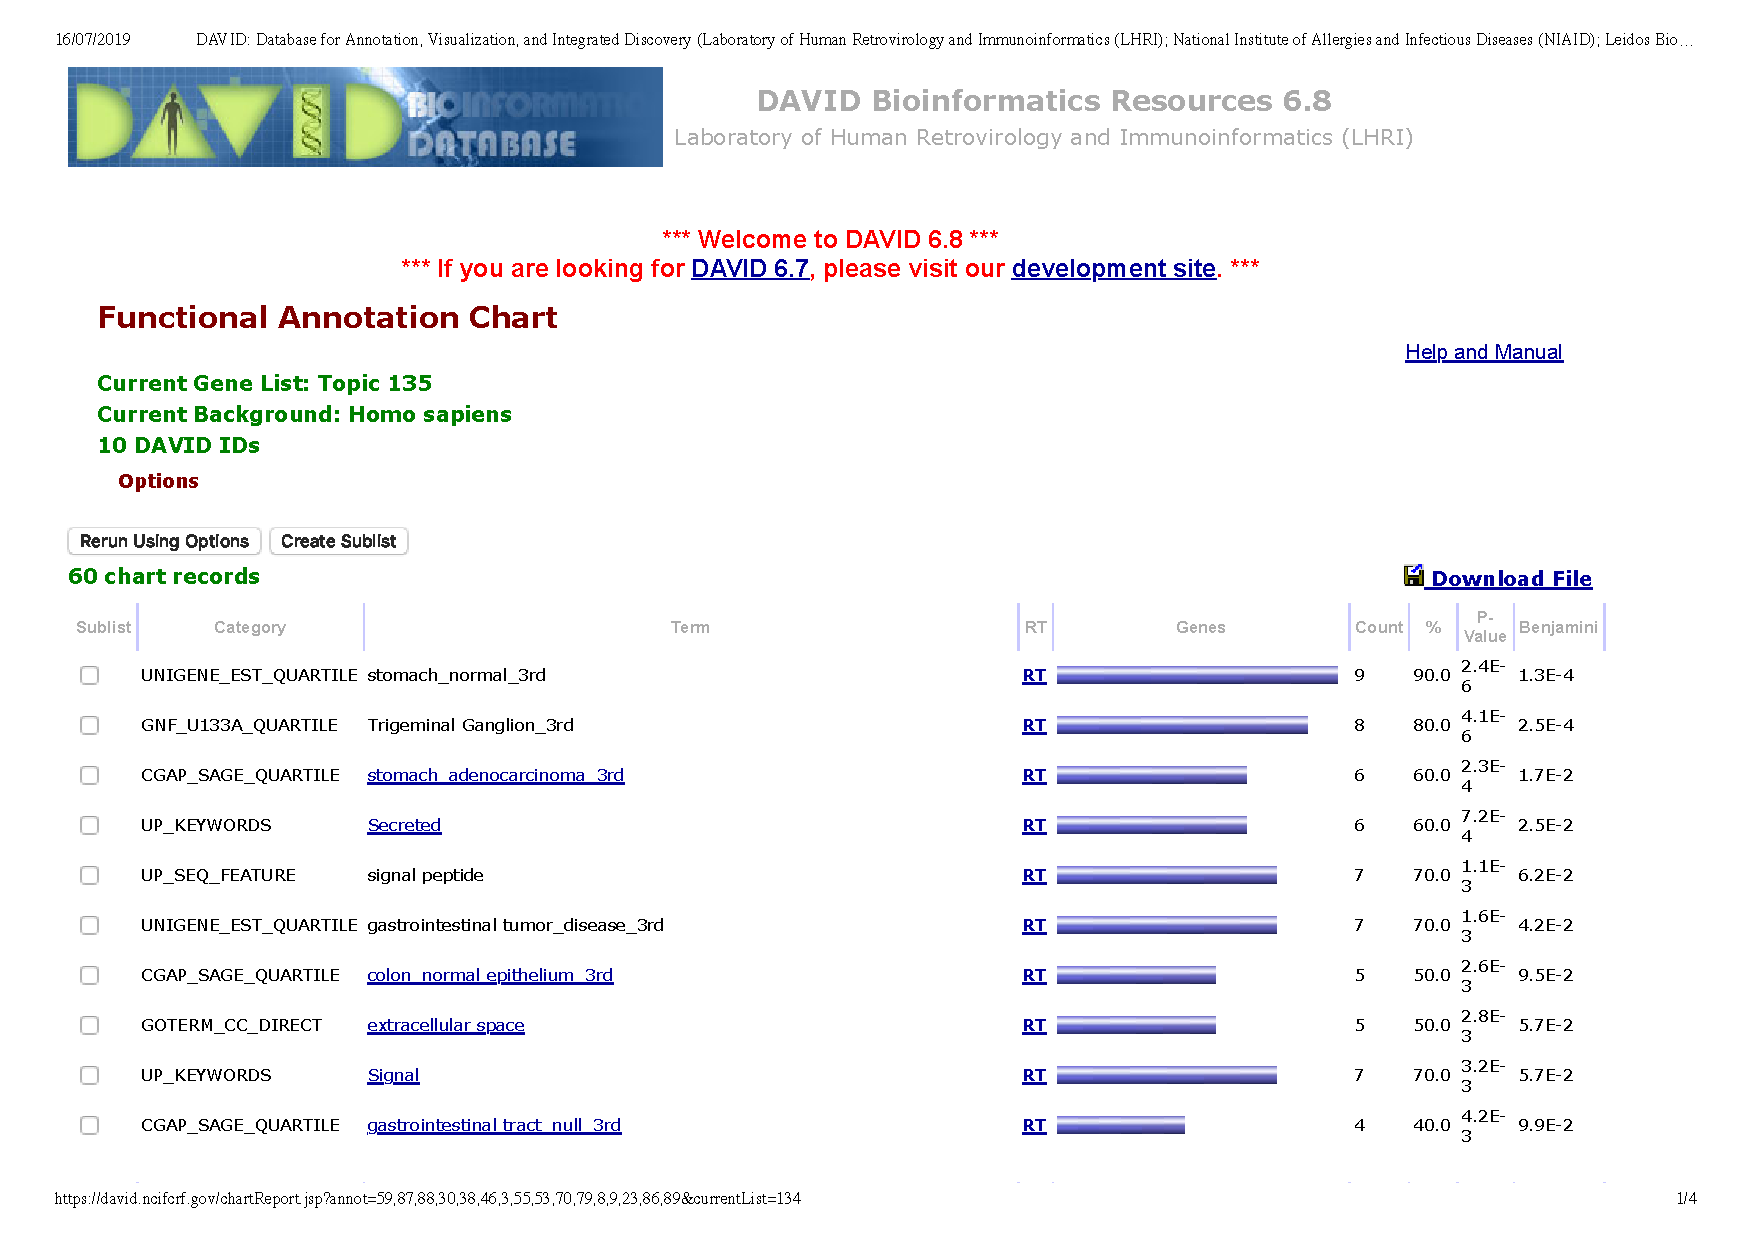
\includegraphics[width=0.8\linewidth]{pictures/topic/merged/DAVID_stomach.pdf}
    \caption{Caption}
    \label{fig:topic/merged/DAVID_stomach}
\end{figure}

%%results
\clearpage
\section{Results}\label{sec:topic/results}
The analysis using topic modelling leads to many interesting results.

The first result achieved is the development of a model that can reproduce the distinction between different tissues from RNA-sequencing datasets. This is evident looking at the cluster composition. Moreover, if one defines more objective metrics based on the entropy the score is quite high, this encouraged further analysis. In particular, in many cases, the model not only reproduces the main tissue classification but was demonstrated that at different layers of the hierarchy even the sub-tissue labels are distinguished. The mutual information score confirms this model's behaviour: tissues are separated at a higher level of the hierarchy and in the deeper layers the sub-tissues are distinguished.

A null model realized shuffling the labels confirms that the results achieved are non-trivial. Studying some quantities such as the fraction of cluster with the same label or the number of labels in a cluster and comparing these with the null models' ones it is possible to affirm that clusters are more homogeneous than expected.

The output of the model presented in this work (hSBM) was compared with more standard approaches such as Latent Dirichlet Allocation and hierarchical clustering. hSBM outputs better results than standard approaches, moreover, it gains higher scores. An interesting fact is that topic modelling (both hSBM and LDA) is better than standard algorithms. This confirms the good quality of a topic model approach and, inside topic models, hSBM seems better than LDA. All algorithms are distant from the null model as highly expected.

It was also demonstrated that not only clustering of the sample was satisfying but even the genes' classification is interesting. If one looks at the block of genes, the so-called topics, enrichment tests confirm that topics represent an interesting group of genes. In particular, some dataset-specific labels were found in GTEx analysis.

In the end, the relationship between samples and topics reveals interesting facts. The distribution of the topic abundance across samples reveals that it is possible to describe the tissue differentiation as a complex mechanism of relationships between genes' expression. This isn't possible using an LDA approach where genes can have either a uniform or peaked distribution. Biologically this means that all genes are necessary everywhere and a fine-tuning of their expression differentiate by tissue.

The sample clustering, topic analysis and the relationship between samples and topics were made on three different datasets. GTEx containing just healthy samples, TCGA containing cancer samples and~\cite{Wang2017} which merged the two. Analysing the dataset with both healthy and diseased samples the differentiation between tissues is still evident and going deeper in the hierarchy the separation involves also the healthy or diseased status. The tissue separation in the firsts layer confirms that what the algorithm does is separating tissues and there isn't a bias involving differences between datasets.
\clearpage
Each of these cases reveals interesting facts. Being able to reproduce GTEx labels is a good benchmark of the quality of the algorithm; to accurately reproduce TCGA labels is the real challenge that can improve scientific community knowledge and here was partially achieved. Analysing both at the same time helps in understanding which genes are somehow involved in cancer development.